
\documentclass{article}

\usepackage{microtype}
\usepackage{graphicx}
\usepackage{subfigure}
\usepackage{booktabs}
\usepackage{array}
\usepackage{comment}
\usepackage{placeins}
\usepackage{hyperref}

\newcommand{\theHalgorithm}{\arabic{algorithm}}

\usepackage[accepted]{icml2026}

\usepackage{amsmath}
\usepackage{amssymb}
\usepackage{mathtools}
\usepackage{amsthm}

\DeclareMathOperator{\ReLU}{ReLU}
\newcommand{\relu}{\ensuremath{\ReLU}}

\newcolumntype{L}[1]{>{\raggedright\arraybackslash}p{#1}}

\usepackage[capitalize,noabbrev]{cleveref}

\theoremstyle{plain}
\newtheorem{theorem}{Theorem}[section]
\newtheorem{proposition}[theorem]{Proposition}
\newtheorem{lemma}[theorem]{Lemma}
\newtheorem{corollary}[theorem]{Corollary}
\theoremstyle{definition}
\newtheorem{definition}[theorem]{Definition}
\newtheorem{assumption}[theorem]{Assumption}
\theoremstyle{remark}
\newtheorem{remark}[theorem]{Remark}

\icmltitlerunning{Dropout Universality: Scaling Laws and Optimal Scheduling at the Edge-of-Chaos}

\begin{document}

\twocolumn[
 \icmltitle{Dropout Universality: Scaling Laws and Optimal Scheduling at the Edge-of-Chaos}

 \icmlsetsymbol{equal}{*}

 \begin{icmlauthorlist}
 \icmlauthor{Lucas Fernandez Sarmiento}{cmu}
 \end{icmlauthorlist}

 \icmlaffiliation{cmu}{Carnegie Mellon University (CMU), Pittsburgh, Pennsylvania, USA}

 \icmlcorrespondingauthor{Lucas Fernandez Sarmiento}{lucasf@andrew.cmu.edu}

 \icmlkeywords{dropout, mean-field theory, edge of chaos, critical scaling, neural network initialization}

 \vskip 0.3in
]

\printAffiliationsAndNotice{Expanded revision, September 22, 2026.}

\begin{abstract}
We develop a mean-field theory of dropout near the edge of chaos, identifying distinct universality classes for smooth and kinked activations. The resulting propagation theory, combined with a regularization-reach heuristic, motivates concentrating dropout near the input. At fixed dropout budget, front-loaded schedules reduce final test loss by \(18\)--\(35\%\) in MLPs and \(4.15\)--\(7.40\%\) in Vision Transformers on CIFAR-10/100, with smaller improvements at the loss minimum. Additional experiments on audio, tabular, and image classification show gains at validation-selected checkpoints, most clearly on Speech Commands, alongside inconclusive results in some Transformer settings. In the CIFAR-10 budget comparison, front-loading also restrains the late rise in test loss while accuracy continues to improve.
\end{abstract}

\section{Introduction}

A deep network needs to preserve distinctions between its inputs while avoiding excessive dependence on particular internal paths. Dropout deliberately corrupts these paths to discourage memorization, which raises a question: how far can useful distinctions propagate through a network that is repeatedly being corrupted? We study this question near the edge of chaos, and ask whether redistributing a fixed amount of dropout across layers can preserve propagation while exposing more of the network to regularization \cite{poole2016exponentialexpressivitydeepneural,schoenholz2017deepinformationpropagation,Bahri2020StatMechDeepLearning,bahri2024leshoucheslecturesdeep}.

Using the representation-group (coarse-graining) language of \cite{roberts2022principlesdeeplearningtheory,bahri2024leshoucheslecturesdeep}, we show that dropout behaves as a relevant perturbation: it displaces the critical fixed point and grows under depth coarse-graining, pushing the dynamics away from criticality and determining the macroscopic phase. Concretely, dropout deforms the correlation map \cite{schoenholz2017deepinformationpropagation} by adding a correlation-independent shift at perfect alignment, so that, with independent masks across inputs, perfect correlation is no longer a fixed point for any nonzero dropout. Thus, even at the edge-of-chaos \cite{sompolinsky1988chaos,packard1988adaptation,bertschinger2004real}, the depth correlation length is finite. We interpret this shift using Landau theory, as an equation of state for the decorrelation order parameter $m \equiv 1-c^\ast$ (with $c^\ast$ the asymptotic inter-signal correlation), derive the resulting scaling laws, and show that smooth and kinked, \relu{}-like activations exhibit the same qualitative phase diagram but different critical scaling in the presence of dropout.

Additionally, we show that the two control parameters (dropout strength and distance to criticality) admit a scaling collapse into a single universal form,\footnote{This is analogous to the homogeneous scaling of connected correlation functions near a critical point; related scaling forms hold for one-particle-irreducible vertex functions after the usual Legendre transform \cite{ZinnJustin2002QFTCritical}.} and we illustrate how these predictions compare with mean-field recursions.

The main conceptual contributions are threefold: first, while dropout was previously shown to destroy the order-to-chaos critical point \cite{schoenholz2017deepinformationpropagation}, we show that the deformed mean-field map still retains a nontrivial $c^\ast<1$ fixed point. This allows us to have a well-defined correlation length recursion even in the presence of dropout, and yields a Landau equation of state for $m=1-c^\ast$ together with a two-parameter scaling collapse. Second, we show that universality classes and scaling laws are set by the analytic structure of activations: smooth and kinked activations have distinct critical exponents (Table~\ref{tab:critical_exponents}), a distinction reflected in their Hermite spectral structure (App.~\ref{sec:var-opt-act}). Since the same Gaussian activation kernels arise beyond MLPs, including CNNs and residual branches (App.~\ref{app:cnn_extension}), we expect the qualitative smooth/kinked split to be a well-motivated heuristic. Third, we treat dropout as a depth-dependent dynamical field; treating classically fixed hyperparameters as fields that can change through the network opens a new dimension for hyperparameter optimization across depth, and potentially over training time.

This work complements prior studies of depth-dependent regularization: stochastic depth drops whole residual blocks with increasing probability \cite{huang2016deep}, curriculum dropout anneals dropout over training time \cite{morerio2017curriculum}, and LayerDrop removes transformer layers for efficiency \cite{fan2019reducing}. Our schedules are spatial depth profiles, so they are complementary to temporal curricula and layer-dropping mechanisms. Qualitatively different edge-of-chaos behavior for smooth and \relu{}-like activations was previously observed in \cite{hayou2019impact}; here we extract the scaling exponents and identify the corresponding universality classes.\footnote{The original notebooks, saved results, and seed-level confidence-interval calculations are available in the \href{https://github.com/luklacasito/icml}{\texttt{icml}} repository. See App.~\ref{app:experimental_info} for the full reproducibility statement.}

\paragraph{Conflict of Interest Disclosure.}
The author declares no financial conflicts of interest related to this work.


\section{Mean-Field Theory Background}
\label{sec:mft_background}
We first state the mean-field assumptions for MLPs, which provide the baseline for the dropout analysis \cite{poole2016exponentialexpressivitydeepneural,schoenholz2017deepinformationpropagation,Bahri2020StatMechDeepLearning,bahri2024leshoucheslecturesdeep}. We consider fully-connected MLPs at random initialization, where preactivations are well-approximated as Gaussian random variables with self-consistently determined statistics (means, variances, covariances). In the strict infinite width limit this Gaussian description becomes exact \cite{Lee2018DNNasGP}, while at large but finite width deviations from Gaussianity can be organized perturbatively in the depth-to-width aspect ratio (schematically $L/N$), as treated comprehensively in \cite{roberts2022principlesdeeplearningtheory,bahri2024leshoucheslecturesdeep}. The intuition behind this treatment is that as we add more activations, through the CLT, the statistics will become more and more Gaussian, approaching this distribution asymptotically in the large N limit.

We consider an MLP of depth $L$, $N_l$ neurons in layer $l$, and an activation $\phi:\mathbb{R}\to\mathbb{R}$ (e.g.\ $\tanh$, \relu{}, \emph{etc.}). We use the standard i.i.d.\ Gaussian initialization
\begin{equation}
W^{l}_{ij}\sim \mathcal{N}\left(0,\frac{\sigma_{w}^{2}}{N_{l-1}}\right), \qquad b^{l}_{i}\sim \mathcal{N}\left(0,\sigma_{b}^{2}\right),
\end{equation}
take the input as $y^{0}_{i;a}=x_{i;a}$, and propagate forward via
\begin{equation}
z^{l}_{i;a}= \sum_{j=1}^{N_{l-1}} W^{l}_{ij} y^{l-1}_{j;a}+b^{l}_{i}, \qquad y^{l}_{i;a}=\phi\left(z^{l}_{i;a}\right),
\end{equation}
where $W^l\in\mathbb R^{N_l\times N_{l-1}}$ and $a$ labels the input. Thus the weight variance is scaled by the number of incoming units. Throughout, expectations $\mathbb{E}[\cdot]$ are over the random weights and biases at initialization, with inputs held fixed. We also use the standard Gaussian measure
\begin{equation}
\int Dz (\cdots)\;\equiv\;\frac{1}{\sqrt{2\pi}}\int_{-\infty}^{\infty}dz e^{-z^{2}/2}(\cdots),
\end{equation}
and similarly for $\int Dz_1 Dz_2$.

In the infinite-width limit this becomes exact layer-by-layer, while at finite width the first layer is exactly Gaussian (being a linear map of fixed inputs) and subsequent layers are only approximately Gaussian, with controlled non-Gaussian corrections parametrized by the depth-to-width ratio \cite{roberts2022principlesdeeplearningtheory}. A fuller treatment of the MFT background is given in App.~\ref{app:mft_primer}.

We track the single-input preactivation variance $q^l_{aa}$, the two-input covariance $q^l_{ab}$, and the induced correlation $c^l_{ab}$. For $l\ge2$, their recursions are
\begin{align}
q^{l}_{aa}&= \sigma_{w}^{2}\int Dz \phi^{2}\left(\sqrt{q^{l-1}_{aa}} z\right)+\sigma_{b}^{2}\\
q^{l}_{ab}&=\sigma_{w}^{2}\int Dz_{1} Dz_{2} \phi(u_{1}) \phi(u_{2})+\sigma_{b}^{2}\\
u_{1}&=\sqrt{q^{l-1}_{aa}} z_{1},\qquad c^{l-1}_{ab}=\frac{q^{l-1}_{ab}}{\sqrt{q^{l-1}_{aa} q^{l-1}_{bb}}},\\
u_{2}&=\sqrt{q^{l-1}_{bb}}\left(c^{l-1}_{ab} z_{1}+\sqrt{1-\left(c^{l-1}_{ab}\right)^{2}} z_{2}\right).
\label{variancerecursion}
\end{align}
The first layer is initialized directly from the inputs, $q^1_{ab}=\sigma_w^2 N_0^{-1}\sum_j x_{j;a}x_{j;b}+\sigma_b^2$.
In the absence of dropout, for a wide array of activations $q^{l}_{ab},c^{l}_{ab}$ settle to fixed points $q^*,c^*$; in particular, there exists a $c^*=1$ fixed point as a straightforward calculation shows. The variance fixed point sets the typical activation scale, while the correlation fixed point describes whether distinct inputs become indistinguishable under depth iteration. We denote the recurrence relation for $c^{l}_{ab}$ by $c^{l}_{ab}=F(c^{l-1}_{ab})$.

To probe its stability, one linearizes the map at $c=1$, defining the (angular) susceptibility
\begin{equation}
\chi_{\perp} \equiv \left.\frac{\partial c^{l}_{ab}}{\partial c^{l-1}_{ab}}\right|_{c_{ab}=1} = \sigma_{w}^{2}\int Dz \big[\phi'(\sqrt{q^{*}} z)\big]^{2}.
\end{equation}
This creates a phase diagram with three regimes: $\chi_{\perp}<1$ is the ordered regime, $\chi_{\perp}>1$ is chaotic, and
 $\chi_{\perp}=1$ defines the critical regime (the so-called "edge-of-chaos"). The depth scale controlling cross-input correlations can become arbitrarily large in the latter, allowing information to penetrate deep into the network. For \relu{}, the criticality condition gives $\sigma_w^2=2$, coinciding with the variance used in He initialization \cite{he2015delvingdeeprectifierssurpassing}\footnote{This is not true for general activations, but rather an idiosyncrasy of \relu{}.} (see App.~\ref{app:mft_primer}), a more fundamental viewpoint than variance preservation.

 This leads to an emergent characteristic depth scale $\xi_c$, which parametrizes both signal propagation and gradient flow. Iterating random affine maps induces an effective coarse-graining in depth akin to renormalization-group flow, called representation group flow in the ML context \cite{roberts2022principlesdeeplearningtheory}; near an attracting correlation fixed point with $r_c=F'(c^*)$ and $0<|r_c|<1$, small correlation deviations decay exponentially with depth,
\begin{equation}
|{c^*-c^l_{ab}}|\propto e^{-l/\xi_{c}}, \qquad \xi_{c}^{-1}\equiv -\log|r_{c}|.
\label{corrq}
\end{equation}
At the marginal point $r_c=1$, nonlinear terms govern the relaxation, which can instead be algebraic.
An analogous correlation length $\xi_q$ controls how quickly single-input norms settle to $q^{*}$. Heuristically, $\xi_{c}$ controls how far distinctions between different inputs survive with depth; in the ordered phase $c^{*}=1$, so $u_{1}^{*}=u_{2}^{*}$ and $\xi_{c}^{-1}=-\log\chi_{\perp}$, hence $\chi_{\perp}\to 1$ implies $\xi_{c}\to\infty$. Consequently, the edge-of-chaos is primarily about $\xi_{c}$ rather than $\xi_{q}$, except in special cases. For \relu{}, the curvature vanishes everywhere away from the origin, leading to a coincidence between $\xi_c$ and $\xi_q$, both diverging as $\chi_{\perp}\to 1$, provided a finite $q^{*}$ exists. This is one concrete reason why \relu{}-style near-critical initializations are comparatively forgiving in practice.

As previously discussed, mean-field theory is an expansion in non-Gaussian corrections suppressed by powers of \(L/N\). Therefore, in our experiments we work in a controlled regime with \(L/N \ll 1\) (i.e., \(N \gg L\)), where the large-width expansion is perturbatively sound \cite{roberts2022principlesdeeplearningtheory}. The correlation length diverges as we approach criticality, amplifying finite-width and other non-Gaussian corrections. Thus, when probing critical power laws with dropout, we keep the dropout rate small but non-negligible: infinitesimal dropout would require prohibitively deep networks to estimate the correlation length and related quantities.

Although we derive these results for MLPs, analogous large-width limits exist elsewhere. CNNs are the canonical convolutional setting \cite{cnnslecun}, and at infinite channel count their covariance recursions again close through Gaussian activation kernels \cite{xiao2018dynamicalisometrymeanfield}. ResNets are especially suggestive: Yang and Schoenholz \cite{yang2017meanfieldresnets} find qualitatively different tanh/\relu{} large-depth behavior. Skip connections alter global depth dynamics, easing the information propagation by injecting the original signal after every layer, changing exponential convergence to subexponential or polynomial laws and allowing norm drift, but each residual branch still inherits the local nonlinear Gaussian kernel. Thus our smooth/kinked universality split offers a possible theoretical explanation for their observed dichotomy; a dropout-deformed ResNet theory is left for future work. For transformers \cite{vaswani2023attentionneed}, related infinite-width attention analyses use large hidden dimension and/or many heads \cite{Hron2020InfiniteAttention}. Because the exponents are controlled by the local analytic structure of this channel, we expect the mechanism to persist when it controls the wide-limit recursion. In Sec.~\ref{subsec:optimal_dropout}, we test this extrapolation in transformers.

In App.~\ref{app:experimental_info} we probe realistic scenarios across architectures, datasets, and schedules. We focus on overparameterized regimes where dropout improves generalization and accuracy, and thus where it is used in practice, and we explicitly study the trade-off between dropout-driven regularization and stable signal propagation. The local-stationary propagation objective introduced below favors sparse, step-like allocation at fixed budget and is permutation invariant in depth. To choose an ordering within this approximation, we use a regularization-reach heuristic: at a common background decay scale, early masks expose more downstream layers to their perturbation. This motivates testing whether the first layers are the most useful place to inject noise.


\section{Universality Classes and Critical Scaling under Dropout}

Dropout \cite{srivastava2014dropout,wager2013dropout} is often used as a regularizer that reduces overfitting by randomly masking activations during training, thereby reducing the network's reliance on any single subset of pathways and discouraging co-adaptation. In the previous literature, dropout was explored in MFT \cite{lee2019mean, schoenholz2017deepinformationpropagation}, but not in the universality class sense. We formalize dropout as multiplicative Bernoulli noise applied post-activation,
\begin{equation}
p^{(\ell)}_{j} \sim \mathrm{Bernoulli}(\rho), \qquad y^{(\ell)}_j \;\mapsto\; \tilde y^{(\ell)}_j \equiv \frac{p^{(\ell)}_{j}}{\rho} y^{(\ell)}_j,
\end{equation}
i.e.\ the standard inverted-dropout convention in which $\mathbb E_p[\tilde y^{(\ell)}_j]=y^{(\ell)}_j$, and hence $\mathbb E_p[\tilde z^{\ell+1}_i\mid W,b,y^\ell]=z^{\ell+1}_i$, so the mean preactivation is invariant to the dropout rate \cite{schoenholz2017deepinformationpropagation}. Throughout, $\rho$ is the keep probability. When comparing two inputs, we draw the dropout masks independently for each input\footnote{Correlated dropout masks can alleviate this detuning: if the same mask is shared across the batch, the \(c=1\) fixed point is preserved and near-critical scaling can be recovered by retuning, but the noise becomes batch coupled and the regularization is correspondingly weaker and more structured. We leave detailed analysis of correlated masks to future work.}; this independence is the source of the decorrelation effect analyzed below.

The smooth/kinked distinction also appears in the Hermite expansion of the activation: $\tanh$ has rapidly decaying coefficients, while \relu{} has a power-law tail. These coefficients determine which derivatives of the correlation map remain finite near perfect alignment, connecting activation regularity to the dropout scaling laws (App.~\ref{sec:var-opt-act}).

Our classification is orthogonal to the scale-invariant vs. non-scale-invariant distinction of \cite{roberts2022principlesdeeplearningtheory}: the multi-scale Hermite spectrum highlighted above is controlled primarily by analytic structure, not by scale invariance per se. The criterion is based on two facts: (a) near-critical scaling laws differ between smooth and kinked activations, and (b) ordinary kinks produce power-law Hermite tails, whereas the smooth examples considered here have much faster decay (Apps.~\ref{ap:exponent_derivations} and~\ref{sec:var-opt-act}).

Consider sending exactly the same input through the same network twice. Without dropout, the two representations remain identical at every layer. With independently sampled dropout masks, different coordinates are erased on the two passes, so even identical inputs no longer produce perfectly aligned representations. Rescaling the surviving activations preserves their mean, but does not restore the missing agreement between the two passes. Perfect alignment therefore ceases to be a fixed point, cutting off the divergence of the depth correlation length at the edge \cite{schoenholz2017deepinformationpropagation}. For a single input, the corresponding variance increase can instead be absorbed into an effective weight variance, $\sigma_w^2\mapsto\sigma_w^2/\rho$.

Introducing multiplicative Bernoulli noise with keep probability $\rho$, the perturbed preactivations read
\begin{equation}
z_i^\ell = \frac{1}{\rho} \sum_{j=1}^{N_{\ell-1}} W_{ij}^\ell p_j^{\ell-1} y_j^{\ell-1} + b_i^\ell.
\end{equation}
The single-input variance recursion becomes
\begin{equation}
\bar{q}_{aa}^{\ell} = \frac{\sigma_{w}^{2}}{\rho} \int Dz \phi^{2}\left( \sqrt{\bar{q}_{aa}^{\ell-1}} z \right) + \sigma_{b}^{2},
\end{equation}
where the bar reminds us that the variance fixed point is shifted by dropout. We denote the (putative) dropout variance fixed point by
\begin{equation}
\bar q^{*} \;=\; \frac{\sigma_w^2}{\rho}\int Dz \phi^2\big(\sqrt{\bar q^{*}} z\big) + \sigma_b^2.
\label{eq:qstar-dropout}
\end{equation}
Assuming this variance fixed point exists and is positive, two distinct inputs $a\neq b$ acquire a dropout shift at perfect alignment. If at some depth $c^{\ell}_{ab}=1$, then at the next layer one finds \cite{schoenholz2017deepinformationpropagation}
\begin{equation}
\bar F_\rho(1)= \bar c^{\ell+1}_{ab} = 1 - \frac{1 - \rho}{\rho \bar{q}^{*}} \sigma_{w}^{2} \int Dz \phi^{2}\left( \sqrt{\bar{q}^{*}} z \right).
\end{equation}
It is therefore natural to define the dropout field
\begin{align}
h &\;\equiv\; 1-\bar F_\rho(1)\nonumber\\
&\;=\; \frac{1-\rho}{\rho \bar q^{*}}\; \sigma_w^2\int Dz \phi^2\big(\sqrt{\bar q^{*}} z\big).
\label{eq:Delta_exact}
\end{align}
For a nondegenerate channel with $\sigma_w^2\int Dz\,\phi(\sqrt{\bar q^*}z)^2>0$, construction gives $\rho<1\Rightarrow h>0$,
so the fixed point at $c^*=1$ is immediately spoiled: even if two inputs are perfectly aligned at some depth, the next layer produces $\bar c_{ab}=1-h<1$. Since we focus on weak dropout, it is useful to perform the small-\(\delta\rho\) expansion. Writing $\delta\rho\equiv 1-\rho$ with $\delta\rho\ll 1$, suppose the no-dropout variance fixed point is positive, isolated and stable, with variance-map derivative $|\chi_q|<1$. The implicit-function theorem then gives $\bar q^*=q^*+\mathcal O(\delta\rho)$, so to leading order
\begin{equation}
h = \delta\rho\; \frac{\sigma_w^2}{\bar q^{*}}\int Dz \phi^2\big(\sqrt{\bar q^{*}} z\big) + \mathcal O(\delta\rho^2).
\label{eq:Delta_weakdrop}
\end{equation}
This variance expansion excludes a marginal variance fixed point. For bias-free \relu{} at unchanged He initialization, dropout gives $q_{\ell+1}=q_\ell/\rho$; its normalized correlation map can still be analyzed without a converged variance, as in App.~\ref{sec:kinks}.
The backward pass has the same source of asymmetry. Let \(\delta^\ell_{j,a}\) be the backpropagated preactivation gradient for input \(a\). With inverted dropout,
\begin{equation}
\delta^\ell_{j,a} = \frac{p^\ell_{j,a}}{\rho} \phi'(z^\ell_{j,a}) \sum_i W^{\ell+1}_{ij}\delta^{\ell+1}_{i,a}.
\end{equation}
For equal hidden-layer widths, let \(G^\ell_{ab}\equiv \mathbb E[\delta^\ell_{j,a}\delta^\ell_{j,b}]\) denote the covariance per coordinate. Under the usual wide-limit gradient-independence approximation, the recursion contains
\begin{equation}
G^\ell_{ab} = \sigma_w^2 \mathbb E\left[ \frac{p^\ell_a p^\ell_b}{\rho^2} \phi'(u_a)\phi'(u_b) \right] G^{\ell+1}_{ab}.
\end{equation}
Thus independent masks give a diagonal factor \(\mathbb E[p_a^2]/\rho^2=1/\rho\) but an off-diagonal factor \(\mathbb E[p_a p_b]/\rho^2=1\). Dropout inflates single-sample gradient variance without similarly inflating cross-sample covariance, mirroring the forward asymmetry that produced \(h\). After normalization this suggests a backward field \(h_\nabla(\rho)\) that moves perfect gradient alignment below one. We do not identify it with the forward field: the backward kernel is built from \(\phi'\), not \(\phi\), and for \relu{} \(\phi'\) is discontinuous. A full dropout-deformed backward critical theory, including finite-width gradient susceptibilities and training-time mask correlations, is left for future work.

\subsection{Landau Theory and Critical Exponents}

For smooth activations, the dropout-deformed correlation edge admits a simple Landau-style description in terms of
three mean-field variables:
\begin{equation}
m \equiv 1-c^*, \qquad t \equiv \chi_\rho-1, \qquad h \equiv 1-\bar F_\rho(1).
\end{equation}
The fields \((m,t,h)\) are chosen to mirror statistical-mechanics notation: \(t\) plays the role of a reduced temperature, \(m\) is the order parameter (magnetization), and \(h\) is an external field conjugate to \(m\) that explicitly biases the system away from perfect alignment.

We assume inverted dropout with keep probability \(\rho\in(0,1]\), with masks drawn i.i.d.\ across units and
independently across inputs. Let \(\bar q^*\) denote the dropout variance fixed point \eqref{eq:qstar-dropout}.
For an activation for which Price's theorem applies and \(\phi',\phi''\in L^2(\mathcal N(0,\bar q^\ast))\) (for instance, \(\phi\in C^2\) with sufficient Gaussian integrability) repeated application of Price's theorem gives the first two
derivatives of the correlation map at perfect alignment,\footnote{The \(\rho\)-dependence is implicit
through \(\bar q^*\). App.~\ref{app:price_dropout} states the derivative identity and its endpoint conditions.}
\begin{align}
\chi_\rho &\equiv \bar F_\rho'(1) = \sigma_w^2\int Dz \big[\phi'(\sqrt{\bar q^{*}} z)\big]^2,
\label{eq:chi_dropout}\\
g_\rho &\equiv \bar F_\rho''(1) = \sigma_w^2 \bar q^{*}\int Dz \big[\phi''(\sqrt{\bar q^{*}} z)\big]^2.
\label{eq:g_dropout}
\end{align}
For the $\mathcal O(m^3)$ remainder used below, we additionally assume that the third application of Price's theorem is valid and that $\phi^{\prime\prime\prime}\in L^2(\mathcal N(0,\bar q^*))$. We take $\bar q^*$ and $g_\rho$ to have finite positive limits near the reference critical point. If \(g_\rho=0\), as for a linear activation, the quadratic Landau term is absent and the leading nonzero term determines a degenerate case rather than the generic smooth universality class.
For kinked, \relu{}-like activations, \(\bar F_\rho''(1)\) is not finite and the analytic expansion below is not the
correct organizing principle; we treat that universality class separately.

For \relu{}, imagine two nearly identical signals arriving on opposite sides of zero: one passes through, while the other is clipped. At a fixed nonzero Gaussian variance and correlation $c$ close to one, the signals have a root-mean-square separation $\mathcal O(\sqrt{1-c})$, so a fraction $\mathcal O(\sqrt{1-c})$ can straddle the kink. Within this small region, their mean squared activation difference is $\mathcal O(1-c)$, giving a contribution $\mathcal O((1-c)^{3/2})$. At the fixed point, where $m=1-c^*$, this produces the $m^{3/2}$ correction, while the smooth class above has an $m^2$ term (App.~\ref{app:tube_argument_kink}).

For the smooth class, the Landau equation of state follows by expanding \(\bar F_\rho(c)\) around \(c=1\). Writing \(c^*=1-m\) with \(0<m\ll 1\) acting as the order parameter,
\begin{align}
\bar F_\rho(1-m)&=\bar F_\rho(1)-\chi_\rho m+\frac{g_\rho}{2}m^2+\mathcal O(m^3)\\
&=(1-h)-\chi_\rho m+\frac{g_\rho}{2}m^2+\mathcal O(m^3),
\end{align}
 imposing the fixed-point condition \(1-m=\bar F_\rho(1-m)\) yields
\begin{equation}
h + t m - \frac{g_\rho}{2} m^2 = 0, \quad\Longleftrightarrow\quad h = \frac{g_\rho}{2} m^2 - t m,
\label{eq:EoS_correct}
\end{equation}
with \(t\equiv \chi_\rho-1\). The physical (nonnegative) solution is
\begin{equation}
m(t,h) \;=\; \frac{t + \sqrt{t^2 + 2 g_\rho h}}{g_\rho}.
\label{eq:m_smooth_solution}
\end{equation}
At the correlation edge \(t=0\), dropout displaces the fixed point by
\begin{equation}
m(0,h) \;=\; \sqrt{\frac{2h}{g_\rho}}.
\label{eq:m_at_edge}
\end{equation}
\begin{table}[h]
\caption{Definitions of critical exponents near the correlation edge in the infinite-width theory ($t,h\to0$). Here $C_{\rm sing}=-\partial_t^2 f_{\rm sing,on}(t,0)$, where $f_{\rm sing,on}$ is the singular Landau potential evaluated at its stable stationary point.}
\label{tab:math_exponents}
\centering
\renewcommand{\arraystretch}{1.8}
\begin{tabular}{lc}
\toprule
Exponent & Mathematical Definition \\
\midrule
$\beta$ & $m \sim t^\beta \quad (h=0,\ t\to0^+)$ \\
$\delta$ & $m \sim |h|^{1/\delta} \quad (t=0)$ \\
$\gamma$ & $\chi_M \equiv \left. \frac{\partial m}{\partial h} \right|_{h \to 0} \sim |t|^{-\gamma}$ \\
$\alpha$ & $C_{\rm sing} \sim t^{-\alpha} \quad (t\to0^+)$ \\
$\nu_t$ & $\xi \sim |t|^{-\nu_t} \quad (h=0)$ \\
$\nu_\rho$ & $\xi \sim |h|^{-\nu_\rho} \quad (t=0)$ \\
$\theta_{\rm rel}$ & $m \sim \ell^{-\theta_{\rm rel}} \quad (t=0, h=0)$ \\
\bottomrule
\end{tabular}
\end{table}

For the \(\alpha\) column we define the singular Landau potential \(f_{\rm sing}\) through the equation of state. In the smooth case,
\begin{equation}
\frac{\partial f_{\rm sing}}{\partial m} = -h-tm+\frac{g_\rho}{2}m^2,
\end{equation}
and in the kinked case,
\begin{equation}
\frac{\partial f_{\rm sing}}{\partial m} = -h-tm+\kappa m^{3/2}.
\end{equation}
Evaluating \(f_{\rm sing}\) on the stable branch at \(h=0\) as \(t\to0^+\) gives \(f_{\rm sing,on}\sim t^3\) for the smooth class and \(f_{\rm sing,on}\sim t^5\) for the kinked class, hence \(\alpha=-1\) and \(\alpha=-3\), respectively.

This square-root power law is our first encounter with a larger family of critical exponents familiar in the physics literature, defined in Table~\ref{tab:math_exponents}. The key exponents for our analysis govern the depth correlation length $\xi_{c,\rho}$, which characterizes how perturbations to input correlations decay with depth at initialization and provides a diagnostic for signal propagation. Their derivations are straightforward but cumbersome, so we collect them in App.~\ref{ap:exponent_derivations} and simply quote the resulting exponent values in Table~\ref{tab:critical_exponents}. For reference, we also list the standard mean-field (Landau) exponents of the Ising universality class \cite{Ising1925,LandauLifshitzStatPhys} and the corresponding mean-field exponents of spin-glass theory \cite{EdwardsAnderson1975,Parisi1979PRL,Parisi1980JPA,Parisi1983PRL} for comparison.

\begin{table}[h]
\caption{Critical exponents for neural network initialization, with statistical-mechanics comparisons. Neural $\nu$ exponents describe depth; the comparison rows use spatial correlation length. Their relaxation entries are omitted because a dynamics must be specified separately. The kinked \(\nu_\rho\) is a normal-form field exponent; ordinary bias-free \relu{} dropout follows the constrained path \(t=-h\) but has the same leading \(\xi\sim h^{-1/3}\) law (App.~\ref{ap:exponent_derivations}).}
\label{tab:critical_exponents}
\centering
\small
\setlength{\tabcolsep}{3pt}
\renewcommand{\arraystretch}{1.25}
\begin{tabular}{@{} l ccccccc @{}}
\toprule
\textbf{Universality Class} & $\boldsymbol{\nu_t}$ & $\boldsymbol{\beta}$ & $\boldsymbol{\theta}_{\rm rel}$ & $\boldsymbol{\gamma}$ & $\boldsymbol{\delta}$ & $\boldsymbol{\nu_\rho}$ & $\boldsymbol{\alpha}$ \\
\midrule
\textbf{Smooth activation} & $1$ & $1$ & $1$ & $1$ & $2$ & $\frac{1}{2}$ & $-1$ \\[6pt]
\textbf{Kinked activation} & $1$ & $2$ & $2$ & $1$ & $\frac{3}{2}$ & $\frac{1}{3}$ & $-3$ \\[6pt]
\textbf{Spin glass (SK MF)} & $\frac{1}{2}$ & $1$ & --- & $1$ & $2$ & $\frac{1}{4}$ & $-1$ \\[6pt]
\textbf{Ising-like} & $\frac{1}{2}$ & $\frac{1}{2}$ & --- & $1$ & $3$ & $\frac{1}{3}$ & $0$ \\
\bottomrule
\end{tabular}
\end{table}

\vspace{0.25em}
\noindent
Figure~\ref{fig:dropout_scaling} summarizes these power laws from direct mean-field recursion and shows where higher-order corrections become visible away from the asymptotic regime.

\begin{figure*}[ht]
 \centering
 
\includegraphics[width=1.0 \textwidth]{figures/theory/critical_exponents.pdf}
\caption{
Critical scaling from the mean-field calculation. The top row shows the depth scale $-1/\log\chi$ on the ordered side, fixed-point decorrelation above the edge, and relaxation at criticality. The bottom row varies the dropout field at $\chi=1$. Dashed lines are log--log fits; quoted errors are regression standard errors on deterministic curves. Finite fitting windows and numerical approximation errors are not included. The tunable \relu{} channel is the formal family specified in App.~\ref{app:experimental_info}, rather than an independently tunable finite-variance \relu{} initialization.}
 \label{fig:dropout_scaling}
\end{figure*}

\subsection{Scaling Collapse and Crossover Region}
A scaling collapse asks whether curves that look different are the same response measured with different rulers. Here, changing the dropout strength changes both the natural scale of decorrelation and the amount of detuning needed to compete with it. Measuring each axis in its corresponding scale brings the different curves onto a common curve determined by the relative strength of dropout and detuning. This correspondence is exact for the leading equation of state \cite{ZinnJustin2002QFTCritical}; farther from criticality, higher-order terms produce visible departures. These include $\mathcal O(m^3)$ corrections in the smooth case, $\mathcal O(m^2)$ corrections in the kinked case, and corrections from the nonlinear microscopic map $h=\Delta(\rho)$.
In practice, experiments are rarely tuned exactly to the correlation edge \(t=0\) while simultaneously taking the dropout field to zero, \(h\to 0\). The useful near-critical description is therefore a two-parameter scaling function.

For smooth activations, the order parameter \(m\equiv 1-c^*\) obeys \eqref{eq:EoS_correct},
\begin{equation}
h = \frac{g_\rho}{2} m^2 - t m, \qquad t \equiv \chi_\rho - 1.
\label{eq:eos_smooth_correct}
\end{equation}
The explicit crossover solution is the physical branch in \eqref{eq:m_smooth_solution}. Define rescaled variables
\begin{equation}
\tilde m \equiv m \sqrt{\frac{g_\rho}{2h}}, \qquad \tilde t \equiv -\frac{t}{\sqrt{2g_\rho h}}.
\label{eq:rescaled_vars_smooth}
\end{equation}
Then all curves collapse onto the universal scaling function
\begin{equation}
\tilde m = \sqrt{1+\tilde t^{2}}-\tilde t.
\label{eq:universal_scaling_function_smooth_correct}
\end{equation}
The crossover scale is
\begin{equation}
|t| \sim \sqrt{g_\rho h}.
\label{eq:crossover_scale_smooth}
\end{equation}
For \(|t| \ll \sqrt{g_\rho h}\), one is in the field-dominated regime
\begin{equation}
m \sim \sqrt{\frac{2h}{g_\rho}}.
\label{eq:field_dominated_smooth}
\end{equation}
For \(|t| \gg \sqrt{g_\rho h}\), the asymptotics depend on the sign of \(t\):
\begin{align}
t<0:\qquad m &\simeq \frac{h}{|t|},\\
t>0:\qquad m &\simeq \frac{2t}{g_\rho} + \frac{h}{t} \cdots.
\end{align}
Thus, at either side of the crossover window the system is either in the linear-response regime on the subcritical side (\(t<0\)), or it sits on the chaotic fixed-point branch on the supercritical side (\(t>0\)).

For kinked activations, the leading non-linearity is non-analytic and the equation of state takes the form (see \eqref{eq:eos_kink_correct}),
\begin{equation}
h=\kappa m^{3/2} - t m + \mathcal O(m^2).
\label{eq:eos_kink_again}
\end{equation}
This implies the scaling form
\begin{equation}
m(t,h) = \left(\frac{h}{\kappa}\right)^{2/3} \mathcal{F}\left(\frac{t}{\kappa^{2/3}h^{1/3}}\right).
\label{eq:m_kink_scaling_form}
\end{equation}
Let
\begin{equation}
u \equiv \frac{t}{\kappa^{2/3}h^{1/3}},
\label{eq:def_u}
\end{equation}
and define \(y(u)\) as the positive real root of
\begin{equation}
y^3 - u y^2 - 1 = 0 \qquad\implies\qquad \mathcal{F}(u)=y(u)^2.
\label{eq:cubic_y_correct}
\end{equation}
The associated crossover scale is
\begin{equation}
|t| \sim \kappa^{2/3} h^{1/3},
\label{eq:crossover_scale_kink}
\end{equation}
showing that kinked activations lie in a distinct universality class from smooth activations. For literal bias-free \relu{} with standard inverted dropout, the microscopic path locks \(t=\rho-1=-h\), so the \(t=0,h>0\) direction is a normal-form field direction rather than a directly independent \relu{} knob. This path nevertheless satisfies \(t/(\kappa^{2/3}h^{1/3})\to0\), hence it enters the same field-dominated regime and retains the leading constrained-path law \(\xi\sim h^{-1/3}\); App.~\ref{ap:exponent_derivations} gives the short derivation and the nonzero-bias caveat.

\begin{figure*}[ht]
 \centering
 
\includegraphics[width=1.0\textwidth]{figures/theory/smooth_scaling_collapse.pdf}
 \caption{
 Two-parameter crossover and scaling collapse for the smooth universality class (tanh), computed from the full mean-field map. Each curve fixes the dropout probability $p=1-\rho$; its field $h$ and curvature $g_\rho$ are recomputed at each point. After rescaling, near-critical points approach the leading equation-of-state curve, while larger fields and decorrelations show departures from it. The kinked counterpart is shown in Fig.~\ref{fig:kinked_collapse}.}
 \label{fig:uni_scaling}
\end{figure*}

Figure~\ref{fig:uni_scaling} shows this collapse for smooth activations. This also clarifies the tanh/\relu{} dichotomy observed in ResNet mean-field theory \cite{yang2017meanfieldresnets}: tanh belongs to the smooth class, where the analytic \(m^2\) term makes weak fields especially important and long correlation lengths are preserved when dropout is kept small; \relu{} belongs to the kinked class, where the \(m^{3/2}\) branch point broadens the crossover window and makes the dynamics more forgiving to imperfect tuning. In short, smooth channels reward keeping the dropout field very weak, while kinked channels tolerate detuning over a wider range; neither class is uniformly preferable.

\subsection{Optimal Dropout Scheduling and Regularization Reach}
\label{subsec:optimal_dropout}

So far we have taken the keep probability to be constant with depth. Since dropout enters as a relevant field that cuts off the depth correlation length even at the correlation edge, it is natural to ask how to allocate a fixed dropout budget across layers so as to preserve near-critical propagation as much as possible. Let us introduce a depth-dependent keep probability $\rho_\ell$ and define the associated dropout field
\begin{equation}
h_\ell \;\equiv\; \Delta(\rho_\ell),
\end{equation}
i.e. the shift of the correlation map at perfect alignment induced by keep probability $\rho_\ell$. If variances have settled so that a scalar map applies at each layer, the exact linear response along the trajectory $c_\ell=\bar F_{\rho_\ell}(c_{\ell-1})$ is
\begin{equation}
\delta c_L=\left[\prod_{\ell=1}^L \bar F_{\rho_\ell}'(c_{\ell-1})\right]\delta c_0.
\end{equation}
To obtain a tractable scheduling objective, we approximate each derivative by its local fixed-point value and freeze the near-critical coefficients $t$ and $g_\rho$ at a common reference. This local-stationary approximation neglects variance transients and the lag between the trajectory and changing fixed points. In the smooth class it gives (see \eqref{eq:lambda_smooth_correct})
\begin{equation}
\lambda(t,h_\ell)\;\simeq\; 1-\sqrt{t^2+2g_\rho h_\ell}.
\end{equation}
For $0<\lambda_\ell\lesssim 1$, this approximates the propagated perturbation by
\begin{equation}
\delta c_L \;\sim\; \prod_{\ell=1}^L \lambda_\ell \delta c_0, \qquad \lambda_\ell \;\equiv\; \lambda(t,h_\ell),
\label{delta_c_dropout_perturb}
\end{equation}
which motivates the following surrogate for the mean decay rate per layer:
\begin{equation}
\xi_{\rm eff}^{-1} \;\equiv\; -\frac{1}{L}\sum_{\ell=1}^L \log\lambda_\ell \;\simeq\; \frac{1}{L}\sum_{\ell=1}^L \sqrt{t^2+2g_\rho h_\ell}.
\end{equation}
At the correlation edge $t=0$, this reduces to
\begin{equation}
\xi_{\rm eff}^{-1}(t=0) \;\simeq\; \sqrt{2g_\rho} \frac{1}{L}\sum_{\ell=1}^L h_\ell^{1/2} \;\propto\; \frac{1}{L}\sum_{\ell=1}^L h_\ell^{1/2}.
\label{eff_corr}
\end{equation}
We now fix a total dropout budget and local bounds,
\begin{equation}
\bar h \;\equiv\; \frac{1}{L}\sum_{\ell=1}^L h_\ell, \qquad 0 \le h_\ell \le h_{\max}.
\end{equation}
The budget above is a budget in the dropout field \(h_\ell\), not directly in the raw dropout probability \(p_{\mathrm{drop},\ell}=1-\rho_\ell\). For weak dropout,
\begin{equation}
\begin{aligned}
h_\ell &= a p_{\mathrm{drop},\ell} + \mathcal O(p_{\mathrm{drop},\ell}^2),\\
a&=\frac{\sigma_w^2}{q^\ast}\int Dz \phi^2(\sqrt{q^\ast}z),
\end{aligned}
\end{equation}
so a fixed \(h\)-budget and a fixed dropout-probability budget agree to leading order. For larger dropout, the nonlinear map \(h_\ell=\Delta(\rho_\ell)\) should be used explicitly.

\begin{figure*}[t]
\centering
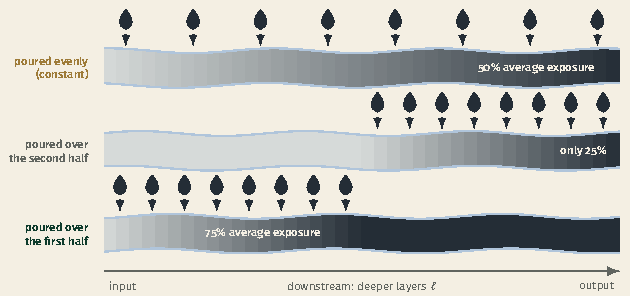
\includegraphics[width=0.93\textwidth]{figures/theory/river_ink.pdf}
\caption{A set amount of ink is distributed along a river with the goal of corrupting every cross section as much as possible. Front-loading and letting the current propagate the ink forward is the way to go. The ink is carried downstream without fading, and the percentages show average exposure along the river.}
\label{fig:river_reach}
\end{figure*}

Maximizing $\xi_{\rm eff}$ is equivalent to minimizing $\xi_{\rm eff}^{-1}$, so in the continuum limit ($x=\ell/L$) we obtain the constrained variational problem
\begin{equation}
\min_{h}\int_0^1 h(x)^{1/2} dx \qquad {\rm s.t.}\qquad \int_0^1 h(x) dx=\bar h.
\end{equation}
Since $h^{1/2}$ is concave, Jensen's inequality gives the maximum at the constant schedule. The chord bound $h^{1/2}\ge h/h_{\max}^{1/2}$ gives the minimum, attained by saturating the box constraint almost everywhere. Equivalently, any schedule that takes values in \(\{0,h_{\max}\}\) with active fraction \(f=\bar h/h_{\max}\) is optimal for the mean-field functional. A front-loaded representative, selected below by regularization reach, is
\begin{equation}
h(x)= \begin{cases} h_{\max}, & 0\le x\le f,\\
0, & f<x\le 1, \end{cases} \qquad f=\frac{\bar h}{h_{\max}},
\end{equation}
where \(x=0\) denotes the input side. All permutations of this saturated set give the same $\xi_{\rm eff}$ in the surrogate; we choose an ordering using the regularization-reach heuristic below. For finitely many layers, at most one layer remains unsaturated to meet the exact budget. These conclusions apply to the leading-order objective with weak $h_{\max}$; abrupt schedules need not track their local fixed points, and the full recurrence need not be permutation invariant. For this representative, uniform dropout yields $\xi_{\rm eff}\sim \bar h^{-1/2}$ while the step schedule gives
\begin{equation}
\frac{\xi_{\rm eff,step}}{\xi_{\rm eff,uniform}} = \sqrt{\frac{h_{\max}}{\bar h}} \;\ge\; 1.
\end{equation}
For kinked activations at $t=0$, one has $\xi^{-1}\propto h^{1/3}$, so the objective becomes $\int_0^1 h(x)^{1/3}dx$, which is also concave and therefore the same conclusion immediately follows.

\paragraph{Where should the ink enter?}
Dropout is used to ``corrupt'' the network so as to prevent it from memorizing certain ``paths'' from input to output. A toy model for understanding how to best corrupt every part of the network with a set amount of damage is to imagine a similar system: a river where a set amount of ink is to be distributed with the goal of corrupting every cross section as much as possible. Reframed this way, it is obvious that front-loading and letting the current propagate the ink forward is the way to go. While this serves as an intuitive explanation, regularization reach makes this intuition explicit.

To make the toy model precise, use normalized depth $x=\ell/L$ and write $j(x)=h(x)/\bar h$ for the injection density, with $\bar h>0$ and $\int_0^1j(x)\,dx=1$. In the limit of negligible attenuation shown in Fig.~\ref{fig:river_reach}, the accumulated exposure at $x$ and its average along the river are
\begin{align}
E(x)&=\int_0^x j(s)\,ds,\\
\bar E&=\int_0^1 E(x)\,dx
       =\int_0^1(1-s)j(s)\,ds.
\end{align}
Uniform injection has $j=1$ throughout; early and late injection have $j=2$ over their respective halves. Thus
\begin{equation}
\bar E_{\rm early}=\tfrac34,\qquad
\bar E_{\rm uniform}=\tfrac12,\qquad
\bar E_{\rm late}=\tfrac14.
\end{equation}
All three schedules deliver the same total ink to the outlet, but expose different amounts of the river along the way.

\paragraph{From the river to the network.}
The river motivates choosing among the saturated profiles with equal $\xi_{\rm eff}$ by maximizing downstream exposure to the perturbation (App.~\ref{app:regularization_reach}). In a network, a mask's influence can weaken as it propagates. Apply dropout only at layer \(\ell\). For masked and clean activations \(\tilde y_k^{(\ell)}\) and \(y_k\) at a later layer \(k\), define their angular decorrelation as
\begin{equation}
\eta_k^{(\ell)}
\equiv
1-\frac{\mathbb E_p[\langle \tilde y_k^{(\ell)},y_k\rangle]}
{\sqrt{\mathbb E_p[\|\tilde y_k^{(\ell)}\|^2]\|y_k\|^2}} .
\end{equation}
Thus \(\eta_k^{(\ell)}=0\) means perfect clean--masked alignment. Immediately after the mask, \(\eta_\ell^{(\ell)}=1-\sqrt{\rho_\ell}=(1-\rho_\ell)/2+\mathcal O((1-\rho_\ell)^2)\), while \(h_\ell=a(1-\rho_\ell)+\mathcal O((1-\rho_\ell)^2)\); hence \(\eta_\ell^{(\ell)}\propto h_\ell\) to leading order. In an ordered background, linearizing the downstream Gaussian channel gives \(\eta_{\ell+r}^{(\ell)}\simeq C h_\ell e^{-r/\xi_c}\), neglecting variance transients. We use a common background $\xi_c$ when comparing mask locations; at an exactly marginal clean channel, higher-order terms instead govern algebraic relaxation.

The readout perturbation \(C h_\ell e^{-(L-\ell)/\xi_c}\) is larger for later dropout, so readout variance is not the front-loading objective. Our scheduling heuristic uses downstream exposure: how much later computation trains while seeing the mask. A mask inserted early is seen, with decaying strength, by many later blocks; a late mask has less time to decay but fewer blocks left to regularize. We therefore define \(\mathcal D_\ell\) as the cumulative downstream exposure from placing dropout at layer \(\ell\), motivating
\begin{align}
\mathcal D_\ell
&\propto h_\ell\sum_{r=1}^{L-\ell}e^{-r/\xi_c} \nonumber\\
&\approx h_\ell\xi_c\left(1-e^{-(L-\ell)/\xi_c}\right)
\equiv h_\ell w_\ell .
\label{eq:regularization_reach}
\end{align}
Under this additive exposure model, \(w_\ell=\xi_c(1-e^{-(L-\ell)/\xi_c})\) decreases with \(\ell\), so maximizing \(\sum_{\ell=1}^L h_\ell w_\ell\) subject to \(\sum_{\ell=1}^L h_\ell=L\bar h\) and \(0\le h_\ell\le h_{\max}\) is a linear program solved by filling the earliest layers first. This is a proposed proxy for regularization; the link from cumulative exposure to generalization remains an empirical question.


\begin{table*}[t]
\centering
\caption{Original paper experiments. Positive changes favor the named profile over uniform. CE reduction is $100(L_U-L_F)/L_U$ using seed means; accuracy gain is in percentage points. Brackets give nominal paired 95\% confidence intervals (Fieller for CE; Student-$t$ for accuracy), conditional on the selected profiles and fixed data split. Profiles were selected by mean final test CE among the historical nonuniform runs, then frozen for the additional seeds; they stay fixed across columns. Pooled intervals do not account for the earlier selection. Final CE and accuracy use the last epoch. Minimum CE averages each seed's lowest recorded test loss; this retrospective endpoint uses test data to choose an epoch, not validation. The first two rows share the same uniform runs. See the main text for the assumptions and selection limits.}
\label{tab:loss_improvements}
\footnotesize
\setlength{\tabcolsep}{4pt}
\renewcommand{\arraystretch}{1.15}
\begin{tabular}{@{}lrlrrr@{}}
\toprule
Experiment & $n$ & Profile & \shortstack{Final CE\\reduction (\%)} & \shortstack{Min. test CE\\reduction (\%)} & \shortstack{Final accuracy\\gain (pp)} \\
\midrule
\shortstack[l]{CIFAR-10\\MLP schedules} & 25 & Step early & \shortstack{$+17.86$\\[-1pt]{\scriptsize $[17.31, 18.41]$}} & \shortstack{$+1.42$\\[-1pt]{\scriptsize $[1.19, 1.65]$}} & \shortstack{$+0.83$\\[-1pt]{\scriptsize $[0.55, 1.11]$}} \\
\shortstack[l]{CIFAR-10\\MLP budget controls} & 25 & Big step & \shortstack{$+22.61$\\[-1pt]{\scriptsize $[22.06, 23.15]$}} & \shortstack{$+2.07$\\[-1pt]{\scriptsize $[1.80, 2.33]$}} & \shortstack{$+1.08$\\[-1pt]{\scriptsize $[0.85, 1.31]$}} \\
\shortstack[l]{CIFAR-10\\ReLU p=0.1} & 10 & Big step & \shortstack{$+34.90$\\[-1pt]{\scriptsize $[34.36, 35.44]$}} & \shortstack{$+2.54$\\[-1pt]{\scriptsize $[2.03, 3.06]$}} & \shortstack{$+1.56$\\[-1pt]{\scriptsize $[1.22, 1.89]$}} \\
\shortstack[l]{CIFAR-10\\GELU p=0.1} & 10 & Big step & \shortstack{$+29.79$\\[-1pt]{\scriptsize $[28.96, 30.61]$}} & \shortstack{$+2.45$\\[-1pt]{\scriptsize $[1.90, 3.00]$}} & \shortstack{$+0.62$\\[-1pt]{\scriptsize $[0.16, 1.08]$}} \\
\shortstack[l]{CIFAR-100\\ViT} & 10 & Linear decreasing & \shortstack{$+4.15$\\[-1pt]{\scriptsize $[3.40, 4.90]$}} & \shortstack{$+1.39$\\[-1pt]{\scriptsize $[0.56, 2.21]$}} & \shortstack{$+0.66$\\[-1pt]{\scriptsize $[0.36, 0.96]$}} \\
\shortstack[l]{CIFAR-10\\ViT both-block ablation} & 10 & Step early & \shortstack{$+7.40$\\[-1pt]{\scriptsize $[5.35, 9.41]$}} & \shortstack{$+1.51$\\[-1pt]{\scriptsize $[0.33, 2.68]$}} & \shortstack{$+0.68$\\[-1pt]{\scriptsize $[0.24, 1.12]$}} \\
\bottomrule
\end{tabular}
\end{table*}


We ask two experimental questions: does moving a fixed amount of dropout toward the input improve performance, and does this advantage remain useful across different datasets and architectures? The CIFAR-10/100 experiments \cite{krizhevsky2009cifar} address the first question by holding the dropout budget fixed (App.~\ref{app:experimental_info}). The broader benchmarks address the second using each cohort's validation protocol for learning rate and dropout strength, allowing mean dropout to differ between profiles. The Vision Transformer experiments \cite{dosovitskiy2021vit} test empirical transfer; the MLP initialization theory does not establish their training dynamics. In the CIFAR comparisons, the largest gains appear at the end of training: final test loss falls by \(18\)--\(35\%\) in MLPs and \(4.15\)--\(7.40\%\) in Vision Transformers (Table~\ref{tab:loss_improvements}). Comparing each run's minimum recorded test loss gives smaller reductions of \(1.39\)--\(2.54\%\). This retrospective minimum uses the test set to choose an epoch; the broader benchmarks instead evaluate test performance at checkpoints chosen using validation loss.

Accuracy counts correct labels, while cross-entropy also measures how much probability they receive. In a binary example, reducing the probability assigned to the correct class from $0.8$ to $0.6$ leaves the prediction correct, but increases its loss from $0.22$ to $0.51$. Conversely, increasingly confident mistakes can outweigh improvements on other examples, allowing accuracy and loss to rise together. We therefore report both metrics. On CIFAR-100, the linearly decreasing profile improves final accuracy from $48.61\%$ to $49.27\%$, alongside the loss comparison.

\paragraph{Behavior after the loss minimum.}
In the 25-seed CIFAR-10 budget comparison (Fig.~\ref{fig:triple_dropout}), the mean test-loss curve under uniform dropout rises from $1.685$ at its minimum (epoch 15) to $2.223$ at epoch 75, whereas the early big-step profile rises from $1.650$ (epoch 29) to $1.721$. These increases are $32.0\%$ and $4.3\%$, respectively, and the big-step model's mean test accuracy improves from $41.88\%$ to $42.92\%$ over epochs 29--75. Front-loading therefore leaves room for classification accuracy to improve while limiting the late deterioration in cross-entropy. This pattern is consistent with reduced overfitting and better late-training generalization in this comparison; whether it comes from reduced memorization would require measuring memorization directly.

The appendices check that this is not a single-run effect: the gains persist across \(\bar h\)-sweeps and large-width sweeps for kinked \relu{} MLPs (App.~\ref{app:sweeps}, Fig.~\ref{fig:mlp_sweeps}), across the smooth GELU activation class (App.~\ref{app:sweeps}, Fig.~\ref{fig:gelu_h_sweep}), and across transformer schedules and component ablations (Figs.~\ref{fig:dropout_regimes_transformer} and~\ref{fig:ablations}). In these CIFAR experiments, the advantage weakens at high dropout or in narrow networks, consistent with the limitations of the small-field, large-width approximation.

\paragraph{Uncertainty across seeds.}
Tables~\ref{tab:loss_improvements} and~\ref{tab:frontloaded_results} report nominal $95\%$ confidence intervals, pairing runs by their recorded seed or original simulation index. Loss reductions use ratios of seed means, with paired Fieller intervals \cite{fieller1954interval}; accuracy gains use paired Student-$t$ intervals in percentage points. Both use $n-1$ degrees of freedom and assume independent seed pairs with approximately bivariate normal losses or normal accuracy differences. We extended the smaller headline comparisons with fresh seeds, freezing their schedules and hyperparameters beforehand: all original CIFAR comparisons now have at least ten pairs, as do all benchmark checkpoint comparisons. Benchmark final endpoints have five or ten pairs, as indicated in the table. These intervals describe seed variation on the recorded split, without adjustment for the earlier profile selection or multiple comparisons, and do not include uncertainty from new data or new splits. All six original CIFAR comparisons have positive minimum-loss and final-accuracy intervals; the MLP schedule and budget-control rows share their uniform runs and should not be counted as independent replications. The appendix retains the original multi-profile cohorts so that the broader comparisons remain visible.

\begin{table*}[t]
\centering
\caption{Frontloaded dropout across tasks. Profiles were selected by lowest mean minimum validation CE among complete paired arms in the historical cohorts, then frozen for the additional seeds. Each profile stays fixed across columns; pooled intervals do not account for the earlier selection. Positive values favor frontloading. CE reduction is $100(L_U-L_F)/L_U$ using seed means; accuracy gain is in percentage points. Brackets give nominal paired 95\% confidence intervals (Fieller for CE; Student-$t$ for accuracy); see the main text for assumptions and selection limits. Checkpoint metrics use each run's minimum-validation-loss checkpoint; final metrics use its last epoch. The $n$ column gives checkpoint/final (C/F) paired seed counts. Where historical final evaluations were absent, final results use only the five additional pairs. The extended Jannis Transformer uses weight decay $10^{-7}$ and fixed mean dropout $0.10$; other rows use zero weight decay and allow profile-specific dropout budgets. Learning rate and mean dropout follow each cohort's validation protocol. Per-epoch test histories were not recorded. Dashes mean missing final test evaluations, not zero change.}
\label{tab:frontloaded_results}
\footnotesize
\setlength{\tabcolsep}{4pt}
\renewcommand{\arraystretch}{1.15}
\begin{tabular}{@{}lrlrrrr@{}}
\toprule
& & & \multicolumn{2}{c}{Validation-selected test} & \multicolumn{2}{c}{Final-epoch test} \\
\cmidrule(lr){4-5}\cmidrule(l){6-7}
Experiment (training $N$) & \shortstack{$n$\\C/F} & Profile & \shortstack{CE reduction\\(\%)} & \shortstack{Accuracy gain\\(pp)} & \shortstack{CE reduction\\(\%)} & \shortstack{Accuracy gain\\(pp)} \\
\midrule
\shortstack[l]{Speech Commands (20,020)\\MLP} & 10/5 & Step early & \shortstack{$+12.56$\\[-1pt]{\scriptsize $[11.36, 13.73]$}} & \shortstack{$+1.72$\\[-1pt]{\scriptsize $[1.28, 2.16]$}} & \shortstack{$+12.59$\\[-1pt]{\scriptsize $[9.95, 15.13]$}} & \shortstack{$+1.71$\\[-1pt]{\scriptsize $[0.78, 2.64]$}} \\
\shortstack[l]{Speech Commands (20,020)\\Transformer} & 10/5 & Big step & \shortstack{$+9.04$\\[-1pt]{\scriptsize $[2.52, 15.24]$}} & \shortstack{$+2.06$\\[-1pt]{\scriptsize $[0.72, 3.41]$}} & \shortstack{$+15.51$\\[-1pt]{\scriptsize $[6.44, 23.04]$}} & \shortstack{$+1.10$\\[-1pt]{\scriptsize $[-0.10, 2.30]$}} \\
\addlinespace[3pt]
\shortstack[l]{Jannis (3,840)\\MLP} & 10/5 & Step early & \shortstack{$+2.60$\\[-1pt]{\scriptsize $[1.44, 3.74]$}} & \shortstack{$+1.56$\\[-1pt]{\scriptsize $[0.94, 2.19]$}} & \shortstack{$+16.23$\\[-1pt]{\scriptsize $[14.83, 17.60]$}} & \shortstack{$+3.03$\\[-1pt]{\scriptsize $[1.96, 4.11]$}} \\
\shortstack[l]{Jannis (3,840)\\Transformer} & 10/5 & Big step & \shortstack{$+0.15$\\[-1pt]{\scriptsize $[-0.62, 0.92]$}} & \shortstack{$+0.32$\\[-1pt]{\scriptsize $[-0.51, 1.15]$}} & \shortstack{$+13.02$\\[-1pt]{\scriptsize $[8.96, 16.81]$}} & \shortstack{$-0.19$\\[-1pt]{\scriptsize $[-1.36, 0.98]$}} \\
\shortstack[l]{Jannis extended (3,840)\\Transformer} & 10/-- & Step early & \shortstack{$-0.27$\\[-1pt]{\scriptsize $[-1.16, 0.61]$}} & \shortstack{$+0.39$\\[-1pt]{\scriptsize $[-0.31, 1.10]$}} & -- & -- \\
\addlinespace[3pt]
\shortstack[l]{Tiny ImageNet (20,000)\\MLP} & 10/5 & Step early & \shortstack{$+2.04$\\[-1pt]{\scriptsize $[1.72, 2.37]$}} & \shortstack{$+1.28$\\[-1pt]{\scriptsize $[0.99, 1.57]$}} & \shortstack{$+21.48$\\[-1pt]{\scriptsize $[19.59, 23.35]$}} & \shortstack{$+0.80$\\[-1pt]{\scriptsize $[0.47, 1.14]$}} \\
\shortstack[l]{Tiny ImageNet (20,000)\\Transformer} & 10/5 & Step early & \shortstack{$+2.21$\\[-1pt]{\scriptsize $[1.69, 2.73]$}} & \shortstack{$+1.49$\\[-1pt]{\scriptsize $[1.06, 1.92]$}} & \shortstack{$+21.06$\\[-1pt]{\scriptsize $[20.27, 21.83]$}} & \shortstack{$+0.73$\\[-1pt]{\scriptsize $[-0.19, 1.66]$}} \\
\shortstack[l]{Tiny ImageNet (80,000)\\MLP} & 10/10 & Step early & \shortstack{$+1.17$\\[-1pt]{\scriptsize $[0.92, 1.42]$}} & \shortstack{$+0.77$\\[-1pt]{\scriptsize $[0.50, 1.05]$}} & \shortstack{$+8.65$\\[-1pt]{\scriptsize $[8.26, 9.04]$}} & \shortstack{$+0.68$\\[-1pt]{\scriptsize $[0.48, 0.88]$}} \\
\shortstack[l]{Tiny ImageNet (80,000)\\Transformer} & 10/10 & Linear decreasing & \shortstack{$+0.76$\\[-1pt]{\scriptsize $[-0.24, 1.76]$}} & \shortstack{$+0.13$\\[-1pt]{\scriptsize $[-0.41, 0.67]$}} & \shortstack{$+1.66$\\[-1pt]{\scriptsize $[0.51, 2.81]$}} & \shortstack{$-0.00$\\[-1pt]{\scriptsize $[-0.41, 0.40]$}} \\
\addlinespace[3pt]
\shortstack[l]{FI-2010 (40,000)\\MLP} & 10/5 & Big step & \shortstack{$+4.25$\\[-1pt]{\scriptsize $[2.57, 5.88]$}} & \shortstack{$+0.81$\\[-1pt]{\scriptsize $[0.38, 1.25]$}} & \shortstack{$+68.23$\\[-1pt]{\scriptsize $[67.30, 69.12]$}} & \shortstack{$-2.48$\\[-1pt]{\scriptsize $[-2.86, -2.09]$}} \\
\bottomrule
\end{tabular}
\end{table*}


\subsection{Front-Loaded Dropout Across Datasets}
\label{sec:extended_benchmarks}

To test how far the scheduling advantage extends beyond CIFAR, we compare MLPs and Transformers on Speech Commands, Jannis, and Tiny ImageNet, together with a financial MLP on FI-2010. These comparisons span audio, tabular classification, and vision, using the depth-12, width-256 configurations detailed in App.~\ref{app:extended_experiments}. Table~\ref{tab:frontloaded_results} reports the test loss and accuracy of validation-selected models, alongside the final-epoch endpoints where they were recorded.

For each run, we retain the checkpoint with the lowest validation cross-entropy. We then choose the reported front-loaded profile by averaging these minimum validation losses across the paired seeds, restricting selection to profiles with complete seed coverage; test loss and accuracy enter only the subsequent comparison with uniform dropout. Most cohorts contain five seeds, while the extended Jannis Transformer comparison contains ten. This is a reanalysis of the saved validation histories, with the original hyperparameter searches and data splits held fixed. The selected profile stays the same across the checkpoint and final columns, so a change of endpoint cannot silently change the model being compared.

The clearest improvement occurs for the Speech Commands MLP: early-step dropout reduces checkpoint test loss by $12.71\%$ relative to uniform, with accuracy increasing from $72.23\%$ to $74.06\%$. Uniform dropout itself reduces loss by $10.82\%$ relative to no dropout, placing this comparison in a regime where regularization already helps. The Transformer gives a smaller, noisier improvement of $4.91\%$ with big-step dropout and an accuracy gain of $1.53$ percentage points; both confidence intervals include zero. For the MLP, the loss-reduction interval is $[11.01,14.36]\%$ and the accuracy-gain interval is $[1.20,2.46]$ percentage points. These audio results use a class-balanced random split of clips from the official training subset, leaving generalization to held-out speakers unresolved.

Jannis provides a tabular comparison with a different learning problem. Validation selects early-step dropout for the MLP, giving a $2.92\%$ reduction in checkpoint test loss and a $1.29$-percentage-point accuracy gain. For the standard Transformer cohort, validation selects big step, whose test-loss improvement is only $0.15\%$. The ten-seed follow-up is effectively a tie: its validation-selected early step increases test loss by $0.27\%$, despite improving accuracy by $0.39$ percentage points. Both Transformer loss intervals include zero, while the MLP interval is $[0.49,5.27]\%$, leaving the MLP as the clearer signal in this tabular comparison.

On Tiny ImageNet, the selected profiles reduce checkpoint loss by $1.94\%$ and $2.17\%$ for the MLP and ViT at 20,000 training examples, and by $1.26\%$ and $1.01\%$ at 80,000 examples. The larger-data MLP still reaches only $7.95\%$ accuracy, compared with $7.09\%$ for uniform, so its relative gain should be read alongside this weak absolute performance. At the final epoch, the corresponding loss reductions are $8.84\%$ and $1.68\%$; the difference from the checkpoint comparison makes clear how much of the final-loss gain develops after the validation optimum. For the 80,000-example ViT, both checkpoint and final loss intervals include zero. The FI-2010 MLP gives a $3.57\%$ checkpoint loss reduction with big-step dropout, with interval $[2.41,4.73]\%$; its $0.67$-percentage-point accuracy gain has an interval spanning zero.

These results compare complete training configurations whose learning rates and dropout strengths follow each cohort's validation protocol; mean dropout can therefore differ between the selected profile and uniform. The fixed-budget CIFAR experiments remain the direct control for allocation. The broader evidence shows a useful but task-dependent advantage, with small effects and losses retained alongside the positive cases. App.~\ref{app:extended_experiments} gives the learning curves and all recorded profiles, including the unrestricted nonuniform comparisons in Table~\ref{tab:benchmark_results}.



\section{Conclusions and Further Scope for Research}
By extending mean-field signal propagation to include multiplicative dropout, we established that activation non-analyticity fundamentally dictates universality. This formalism yields a Landau equation of state for the decorrelation order parameter, a universal two-parameter scaling collapse, and distinct critical exponents for smooth versus kinked channels. Mean-field theory is often best at clarifying the mechanisms inside wide networks, and less often at producing directly testable design rules; here it motivates one such rule. Treating dropout as a depth-dependent field gives a local-stationary propagation objective favoring saturated allocation, and an additive regularization-reach heuristic places that allocation near the input. Their use for abrupt schedules and trained networks is tested empirically. These schedules reduce final test loss by \(18\)--\(35\%\) in MLP settings and by \(4\)--\(6\%\) in Vision Transformer settings relative to constant dropout at the same budget (Table~\ref{tab:loss_improvements}), with secondary accuracy gains and no extra computational cost. Comparing minimum recorded test loss gives smaller reductions of \(0.9\)--\(2.5\%\) for the same schedules. The growth of the advantage during continued training is itself a striking result: in the CIFAR-10 budget comparison, front-loading substantially restrains the late rise in test loss while accuracy continues to improve, suggesting that its practical benefit includes limiting overfitting after the loss minimum. The broader comparisons select checkpoints and profiles from validation loss and show smaller, task-dependent gains, including losses to uniform dropout in the extended Jannis Transformer cohort. Extending this mean-field analysis to attention mechanisms and incorporating finite-width corrections are natural directions for future work.

\section{Limitations}
Our analysis is the leading-order, large-width description: finite-width corrections, controlled perturbatively by \(L/N\), are not computed explicitly. They can accumulate with depth; we have not established whether they preserve the leading exponents or how they change a useful scheduling profile. The scheduling objective also freezes local coefficients and replaces trajectory-dependent derivatives by stationary values, while the reach argument assumes additive exposure at a common decay scale. Finite dropout, multiple masks and feature learning can change both approximations.

Architectural scope is also restricted. We treat dropout most explicitly for MLPs; App.~\ref{app:cnn_extension} argues that infinite-channel CNNs and residual branches inherit the same smooth/kinked split through the local Gaussian kernel, but we do not derive the full spatial-mode CNN Landau theory, run CNN experiments, or develop a dropout-deformed ResNet theory. Skip connections in particular modify large-depth propagation while preserving the local channel, so promoting residual-branch strength to a control parameter would put the Transformer experiments on firmer footing.

Finally, the theory is an initialization theory of \emph{forward} correlation dynamics. We give the leading backward covariance recursion and note that dropout creates the same diagonal/off-diagonal asymmetry for gradients, but do not develop the full backward critical theory (finite-width gradient susceptibilities, training-time mask correlations, feature-learning effects), nor do we model how observables evolve after feature learning substantially reshapes representations, e.g.\ in catapult regimes \cite{zhu2024quadraticcatapult}. Extending the same approach to training-time regularizers, dropout warm-up, adaptive schedules, \(L^2\) penalties, or broader scaling-law questions \cite{Bahri2024ExplainingScalingLaws} is a natural direction for future work.

\noindent\emph{Acknowledgments.} The author thanks Riccardo Penco for support and discussions, and the anonymous ICML reviewers for feedback that sharpened the scheduling discussion and the treatment of the kinked-class scaling path. This work is partially supported by the U.S. Department of Energy under grant DE-SC0010118.

\section*{Reproducibility Statement}
The repository linked in the introduction contains the original notebooks and saved results, the manuscript source, and the paired seed endpoints and analysis script underlying Tables~\ref{tab:loss_improvements} and~\ref{tab:frontloaded_results}. App.~\ref{app:experimental_info} reports the original run counts, hyperparameters, dataset splits, hardware, and sweep details. App.~\ref{app:extended_experiments} reports the additional benchmark and profile-pilot evidence, including incomplete coverage. The \texttt{benchmarks/} directory contains the retained benchmark training and data-preparation code, frozen profile configurations and split identifiers; App.~\ref{app:benchmark_protocols} documents their protocols and the unrecovered settings in the standalone financial study. The two main gain tables report nominal $95\%$ confidence intervals; existing curve bands and $\pm$ summaries retain their SEM convention. The mean-field fits use deterministic recursion code from the same repository and report fit standard errors separately. The CIFAR-100 archive lacks the configuration needed to verify all reported settings (Table~\ref{tab:vit_config}).

\section*{Impact Statement}
The main practical benefit is improved performance at fixed training cost, or potentially reduced training cost when targeting a fixed performance level. We do not anticipate additional ethical risks.


\bibliography{bibliography}
\bibliographystyle{icml2026}

\newpage
\onecolumn

\appendix

\section{Mean-Field Background and Dropout Recursions}

\subsection{Notation Guide}
\label{app:notation}

The same few letters carry several nearby meanings, so we collect the main conventions here.
\begin{table}[h]
\caption{Notation used across the main text and appendices.}
\label{tab:notation_guide}
\centering
\small
\begin{tabular}{@{}ll@{}}
\toprule
Symbol & Meaning \\
\midrule
\(\rho_\ell\) & keep probability in layer \(\ell\) \\
\(p_{\mathrm{drop},\ell}=1-\rho_\ell\) & raw dropout probability \\
\(p_j^{(\ell)}\) & Bernoulli dropout mask variable \\
\(m=1-c^\ast\) & decorrelation order parameter at the fixed point \\
\(m_\ell=1-c_\ell\) & depth-dependent decorrelation used in relaxation laws \\
\(\chi_\perp\), \(\chi_1\) & no-dropout angular susceptibility at \(c=1\) \\
\(\chi_\rho\) & dropout-deformed angular susceptibility \(\bar F_\rho'(1)\) \\
\(\chi_M\) & response susceptibility \(\partial m/\partial h\) \\
\(\chi\), \(\chi_q\) & generic Hermite/angle susceptibility and variance-channel susceptibility \\
\(\theta_{\rm rel}\) & relaxation exponent, \(m_\ell\sim \ell^{-\theta_{\rm rel}}\) \\
\bottomrule
\end{tabular}
\end{table}
\FloatBarrier

\subsection{Mean-Field Theory Primer}
\label{app:mft_primer}

Even the Standard Model of physics, with only a few dozen empirical parameters, invites the feeling that some deeper organizing principle is yet to be found. Fermi made the same point more sharply to Dyson by quoting von Neumann: ``With four parameters I can fit an elephant, and with five I can make him wiggle his trunk'' \cite{Dyson2004Fermi}. Modern machine learning pushes this worry to an extreme: parameters are abundant, so understanding cannot mean tracking each weight individually. A pressing question in modern ML literature is what set of parameters or effective fields can give a useful description of the network's behavior, and how to derive such a description from the microscopic model.

Mean-field theory gives one such effective description: instead of tracking every neuron and every random weight, one tracks a small number of self-consistent fields. In the signal-propagation version used here, those fields are variances, covariances, and correlations. This is the deep information propagation line of mean-field theory \cite{poole2016exponentialexpressivitydeepneural,schoenholz2017deepinformationpropagation}, with broader background in statistical-mechanics treatments of deep learning \cite{Bahri2020StatMechDeepLearning,bahri2024leshoucheslecturesdeep}. The same infinite-width covariance recursion can also be read as the NNGP kernel recursion \cite{Lee2018DNNasGP}; we use the MFT language because our questions concern fixed points, susceptibilities, correlation lengths, and critical exponents rather than the induced function-space prior or training dynamics.

Section~\ref{sec:mft_background} gives the main-body version of the signal-propagation story. Here we only fix notation and record the elementary steps used later in the appendices. For a depth-$L$ MLP with activation $\phi:\mathbb R\to\mathbb R$, weights and biases are initialized as
\begin{equation}
W^{l}_{ij}\sim \mathcal{N}\left(0,\frac{\sigma_{w}^{2}}{N_{l-1}}\right), \qquad b^{l}_{i}\sim \mathcal{N}\left(0,\sigma_{b}^{2}\right),
\end{equation}
and propagated by
\begin{equation}
z^{l}_{i;a}= \sum_{j=1}^{N_{l-1}} W^{l}_{ij} y^{l-1}_{j;a}+b^{l}_{i}, \qquad y^{l}_{i;a}=\phi\left(z^{l}_{i;a}\right),
\end{equation}
where $W^l\in\mathbb R^{N_l\times N_{l-1}}$, $y^0=x$, and $a$ labels the input. We write
\begin{equation}
\int Dz (\cdots)=\frac{1}{\sqrt{2\pi}}\int_{-\infty}^{\infty}dz e^{-z^{2}/2}(\cdots),
\end{equation}
and use the same convention for multiple Gaussian variables.

The Gaussian closure comes from the fact that each preactivation is a sum of many independently initialized weighted inputs. In the infinite-width limit this central-limit effect becomes exact layer-by-layer, while finite-width corrections are organized perturbatively in the depth-to-width aspect ratio, schematically $L/N$ \cite{roberts2022principlesdeeplearningtheory}. For $l\ge2$, the single-input variance and two-input covariance recursions are the closed equations already quoted in Sec.~\ref{sec:mft_background}:
\begin{align}
q^{l}_{aa}&=\sigma_{w}^{2}\int Dz \phi^{2}\left(\sqrt{q^{l-1}_{aa}} z\right)+\sigma_{b}^{2},\nonumber\\
q^{l}_{ab}&=\sigma_{w}^{2}\int Dz_{1} Dz_{2} \phi(u_{1}) \phi(u_{2})+\sigma_{b}^{2},\nonumber\\
u_{1}&=\sqrt{q^{l-1}_{aa}} z_{1},\qquad c^{l-1}_{ab}=\frac{q^{l-1}_{ab}}{\sqrt{q^{l-1}_{aa} q^{l-1}_{bb}}},\nonumber\\
u_{2}&=\sqrt{q^{l-1}_{bb}}\left(c^{l-1}_{ab}z_{1}+\sqrt{1-\left(c^{l-1}_{ab}\right)^{2}} z_{2}\right).
\end{align}
Once the variance relaxes to $q^*$, these equations induce a one-dimensional correlation map $c^l_{ab}=F(c^{l-1}_{ab})$. Without dropout, perfect alignment is a fixed point, $F(1)=1$. Its linear stability is controlled by the angular susceptibility
\begin{equation}
\chi_{1}=\left.\frac{\partial c^{l}_{ab}}{\partial c^{l-1}_{ab}}\right|_{c_{ab}=1}=\sigma_{w}^{2}\int Dz \big[\phi'(\sqrt{q^{*}} z)\big]^{2},
\end{equation}
called $\chi_\perp$ in the main text and in \cite{roberts2022principlesdeeplearningtheory}. The ordered, chaotic, and critical regimes correspond to $\chi_1<1$, $\chi_1>1$, and $\chi_1=1$ respectively; the last case is the edge-of-chaos, where the cross-input correlation length can diverge.

The usual He initialization follows from this criterion in the special case of \relu{}. Since $\phi'(z)=\theta(z)$ almost everywhere,
\begin{equation}
\int Dz \big(\phi'(\sqrt{q^{*}}z)\big)^2=\frac12,
\qquad \chi_1=1 \Longrightarrow \sigma_w^2=2,
\end{equation}
which is the variance-$2/N$ initialization. The same example also shows why variance preservation and correlation criticality are not identical: for \relu{},
\begin{equation}
q^{l}_{aa}=\frac{\sigma_w^2}{2} q^{l-1}_{aa}+\sigma_b^2,
\end{equation}
so with nonzero bias the finite-$q^*$ condition requires $\sigma_w^2<2$, while exact angular criticality sets $\sigma_w^2=2$. In practice one either sets biases to zero or works slightly subcritical to keep the variance scale finite.

Finally, the correlation length used throughout the paper is obtained by linearizing the correlation map around its fixed point. With $r_c=F'(c^*)$ and $0<|r_c|<1$, small deviations obey
\begin{equation}
|c^*-c^l_{ab}|\propto e^{-l/\xi_c},\qquad \xi_c^{-1}=-\log|r_c|.
\end{equation}
The analogous variance length $\xi_q$ tracks relaxation of $q^l_{aa}$ to $q^*$, but the edge-of-chaos phenomenon is primarily controlled by $\xi_c$: it measures how many layers preserve distinctions between different inputs. This is the scale deformed by dropout in the main analysis.
\FloatBarrier

\subsection{Derivation of Correlation Map and Derivatives with Dropout}\label{app:price_dropout}

Fix the positive dropout-shifted variance \(\bar q^*\) from \eqref{eq:qstar-dropout}, and let \((u_1,u_2)\) be centered Gaussian with marginal variance \(\bar q^*\) and correlation \(c\). Independent inverted-dropout masks across inputs give the normalized map
\begin{equation}
\bar F_\rho(c)=\frac{\sigma_w^2\mathbb E_c[\phi(u_1)\phi(u_2)]+\sigma_b^2}{\bar q^*},
\qquad h=1-\bar F_\rho(1),
\label{eq:Frho_def_app}
\end{equation}
with \(h\) given by \eqref{eq:Delta_exact}.

Assume \(\phi\in C^2\) and \(\phi,\phi',\phi''\in L^2(\mathcal N(0,\bar q^*))\). Price's theorem \cite{Price1958GaussianInputs,Voigtlaender2021Price}, applied at fixed \(\bar q^*\), states that for \(|c|<1\),
\begin{equation}
\frac{\mathrm d^k}{\mathrm dc^k}\mathbb E_c[\phi(u_1)\phi(u_2)]
=(\bar q^*)^k\mathbb E_c[\phi^{(k)}(u_1)\phi^{(k)}(u_2)],
\qquad k=1,2.
\end{equation}
Strong continuity of Gaussian correlation operators in \(L^2\) then justifies \(c\to1^-\), giving the one-sided derivatives
\begin{align}
\bar F_\rho'(1^-)&=\sigma_w^2\int Dz\,[\phi'(\sqrt{\bar q^*}z)]^2=\chi_\rho,\\
\bar F_\rho''(1^-)&=\sigma_w^2\bar q^*\int Dz\,[\phi''(\sqrt{\bar q^*}z)]^2=g_\rho,
\end{align}
as used in Eqs.~\eqref{eq:chi_dropout}--\eqref{eq:g_dropout}. The boundary passage requires the stated Gaussian square-integrability conditions; the theorem for nondegenerate \(|c|<1\) alone does not establish finite derivatives at perfect alignment.

\FloatBarrier

\subsection{Extensions to Infinite-Channel CNNs and ResNets}
\label{app:cnn_extension}

We briefly discuss extensions to architectures not treated in the main analysis. Although our derivation is for MLPs, the universality-class mechanism is tied to the local Gaussian kernel rather than to the MLP architecture itself. Other architectures introduce additional structure that can change the exact exponents, but the qualitative smooth-versus-kinked distinction should remain when the same local channel controls the wide-limit recursion.

For example, the same local channel which appears in MLPs re-emerges in infinite-width CNNs when the number of channels is taken to infinity: preactivations at different spatial positions become jointly Gaussian across channels, and the covariance recursion composes the same bivariate Gaussian activation expectation with a linear operator that averages over convolutional filter offsets \cite{cnnslecun,xiao2018dynamicalisometrymeanfield}. In schematic form, a spatial covariance \(K^\ell_{\alpha\beta}(x,x')\) evolves as \(K^{\ell+1}=\sigma_b^2+\sigma_w^2\mathcal A[V_\phi(K^\ell)]\), where \(V_\phi\) is the scalar Gaussian channel analyzed above and \(\mathcal A\) is the convolutional averaging operator. Independent dropout shifts the single-input variance entering \(V_\phi\) as in the fully connected case, while the cross-input covariance is still controlled by the same bivariate expectation. Therefore, for an isolated leading spatial mode, convolution changes the relevant eigenvalue and mode shape but not the local smooth-versus-kinked non-analyticity: smooth activations retain the analytic Landau equation, while \relu{}-like kinks retain the \(m^{3/2}\) branch point. A complete CNN theory would promote \(m\) to a spatial covariance-mode amplitude and track boundary conditions, pooling, and degeneracies of \(\mathcal A\).

ResNets modify depth dynamics in a complementary way: skip connections can change exponential convergence to subexponential or polynomial behavior, and norms may drift rather than relax to a fixed point \cite{yang2017meanfieldresnets}. Still, the residual branch evaluates the same nonlinear Gaussian channel \(V_\phi\), so the local analytic distinction is unchanged. The tanh/\relu{} asymptotic split observed in \cite{yang2017meanfieldresnets} is consistent with our smooth/kinked classes; a dropout-deformed ResNet theory would additionally track residual-branch strength and norm drift.

\FloatBarrier

\subsection{Regularization-Reach Derivation}
\label{app:regularization_reach}

The local-stationary propagation surrogate is invariant under permutations of the depth profile \(h_\ell\), so it fixes a saturated allocation while leaving its ordering open. We propose choosing that ordering by asking how much downstream computation sees a dropout perturbation before it is absorbed, using a common background decay scale and an additive exposure model.

First apply dropout only at layer \(\ell\). Write \(\tilde y_k^{(\ell)}\) for the masked trajectory and \(y_k\) for the clean trajectory. We measure the size of the perturbation at layer \(k\) by the clean-vs.-masked angular decorrelation
\begin{equation}
\eta_k^{(\ell)}
\equiv
1-\frac{\mathbb E_p[\langle \tilde y_k^{(\ell)},y_k\rangle]}
{\sqrt{\mathbb E_p[\|\tilde y_k^{(\ell)}\|^2]\|y_k\|^2}}.
\end{equation}
Here \(\eta_k^{(\ell)}=0\) means the two trajectories are perfectly aligned at layer \(k\). Immediately after the mask,
\begin{equation}
\eta_\ell^{(\ell)}
=1-\sqrt{\rho_\ell}
=\frac{1-\rho_\ell}{2}+\mathcal O((1-\rho_\ell)^2).
\end{equation}
The dropout field used in the main text is the same small parameter up to a constant:
\begin{equation}
h_\ell=a(1-\rho_\ell)+\mathcal O((1-\rho_\ell)^2),
\qquad
a=\frac{\sigma_w^2}{q^\ast}\int Dz\,\phi^2(\sqrt{q^\ast}z),
\end{equation}
so \(\eta_\ell^{(\ell)}\propto h_\ell\) to leading order. This constant of proportionality does not affect the scheduling optimizer.

Next, we propagate this perturbation downstream. For \(k>\ell\), the clean-vs.-masked pair is governed by the same wide-limit Gaussian correlation channel as a two-input pair, up to variance-relaxation corrections. Linearizing around an ordered background fixed point gives
\begin{equation}
\eta_{\ell+r}^{(\ell)}
\simeq C h_\ell e^{-r/\xi_c},
\end{equation}
where \(r\) is the number of downstream layers and \(C\) is independent of \(h_\ell\) to leading order. Here $\xi_c$ is the background correlation length, held fixed across mask locations. At an exactly critical clean channel the linear multiplier is one, and higher-order terms produce algebraic relaxation. If we only looked at the final readout, we would get \(C h_\ell e^{-(L-\ell)/\xi_c}\). This is larger for later dropout, because late perturbations have fewer layers over which to decay. That is why readout variance is not the object that explains front-loading.

For scheduling, we use the amount of downstream computation exposed to the mask as a proxy for regularization. We assume that a later layer's exposure is proportional to the remaining mask-induced decorrelation and add these exposures across layers. This assumption does not establish a corresponding improvement in generalization, and interactions between several masks or changes during training may alter it. We denote this cumulative exposure by \(\mathcal D_\ell\). It is not additional dropout strength; it is the downstream sum of the remaining perturbations, proportional to \(\sum_{r=1}^{L-\ell}\eta_{\ell+r}^{(\ell)}\).

Substituting the exponential decay into this exposure sum gives
\begin{equation}
\mathcal D_\ell
\;\propto\;
h_\ell\sum_{r=1}^{L-\ell}e^{-r/\xi_c}
\;\approx\;
h_\ell\int_0^{L-\ell}e^{-s/\xi_c}\,ds
\;=\;
h_\ell\xi_c\left(1-e^{-(L-\ell)/\xi_c}\right)
\;\equiv\;
h_\ell w_\ell.
\end{equation}
The approximation replaces the discrete sum by its continuum integral; using the exact geometric sum changes only constants and leaves the same monotone ordering. The weight \(w_\ell=\xi_c(1-e^{-(L-\ell)/\xi_c})\) decreases with \(\ell\): earlier masks are visible to more downstream layers before they are absorbed (Fig.~\ref{fig:regularization_reach}).

 Within the propagation surrogate, every permutation of the same saturated dropout set pays the same cost. We choose the permutation that gives the largest downstream exposure under the preceding assumptions:
\begin{equation}
\max_{\{h_\ell\}}\sum_{\ell=1}^L h_\ell w_\ell
\qquad
\text{s.t.}
\qquad
\sum_{\ell=1}^L h_\ell=L\bar h,
\qquad
0\le h_\ell\le h_{\max}.
\end{equation}
This is a linear program. Since \(w_1>w_2>\cdots>w_L\), it is solved by filling the largest weights first:
\begin{equation}
h_\ell^\star=
\begin{cases}
h_{\max}, & 1\le \ell\le k,\\
r, & \ell=k+1\le L,\\
0, & \ell>k+1,
\end{cases}
\qquad
k=\left\lfloor\frac{L\bar h}{h_{\max}}\right\rfloor,
\quad r=L\bar h-kh_{\max}.
\end{equation}
The residual $r$ enforces the budget when $L\bar h/h_{\max}$ is not an integer. This exposure model selects a front-loaded step. It predicts that sliding a fixed saturated block $B$ toward later layers reduces $\sum_{\ell\in B}w_\ell$; whether performance follows that ordering is an empirical test of the heuristic.

\begin{figure}[t]
\centering
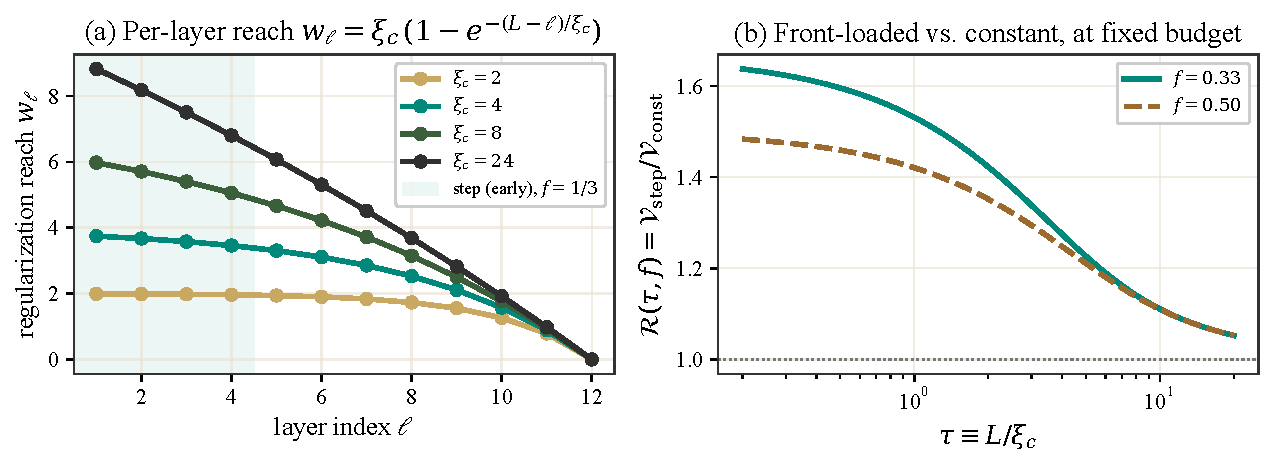
\includegraphics[width=\linewidth]{figures/theory/regularization_reach.pdf}
\caption{Regularization-reach weights at fixed network depth \(L=12\). (a)~Per-layer weight \(w_\ell=\xi_c(1-e^{-(L-\ell)/\xi_c})\) is monotone decreasing in \(\ell\) for any \(\xi_c\); the linear program over the dropout budget therefore fills the smallest-\(\ell\) layers first (shaded: step-early with \(f=1/3\)). For \(L\ll\xi_c\) the reach is essentially linear in \(L-\ell\); for \(L\gg\xi_c\) it saturates at \(\xi_c\). (b)~Ratio \(\mathcal R(\tau,f)=\mathcal V_{\rm step}/\mathcal V_{\rm const}\) of front-loaded to constant schedules at fixed budget, with \(\tau\equiv L/\xi_c\). Here $\mathcal V$ denotes summed exposure at a common background $\xi_c$. In this continuum comparison the ratio approaches $2-f$ as $\tau\to0$ and one as $\tau\to\infty$.}
\label{fig:regularization_reach}
\end{figure}

\FloatBarrier


\section{Critical Exponents and Non-Analyticity}
\label{ap:exponent_derivations}

The Hermite decomposition in App.~\ref{sec:hermite} diagnoses which expansion is valid here. In the Gaussian channel,
\begin{equation}
F(c)=\frac{\sigma_w^2\sum_{n\ge0}a_n^2 c^n+\sigma_b^2}{q^*}.
\end{equation}
The smooth-class derivative moments make this series differentiable to the order needed at $c=1$, giving the finite-order Taylor/Landau equation below. This does not require analyticity or convergence of an infinite Taylor series. A kink produces a power-law Hermite tail, so high-degree modes contribute collectively as \(c\to1\); the Taylor expansion is replaced by the branch-point term \(m^{3/2}\), which is the source of the kinked exponents.

\subsection{Smooth Networks}

The standard static exponents follow directly from \eqref{eq:EoS_correct}. Along the critical isotherm \(t=0\),
\begin{equation}
h=\frac{g_\rho}{2}m^2 \qquad\Rightarrow\qquad m\sim h^{1/2},
\end{equation}
so \(\delta=2\). The analogue of the magnetic susceptibility is \(\chi_M(t)\equiv \left.\partial m/\partial h\right|_{h\to 0}\).
On the subcritical side \(t<0\), the analytic branch satisfies \(m\simeq -h/t\), hence \(\chi_M(t)\sim |t|^{-1}\) and \(\gamma=1\).
Along \(h=0\), the physical branch is \(m=0\) for \(t\le 0\) and \(m=2t/g_\rho\) for \(t\ge 0\), so \(m\sim t\) as \(t\to 0^+\) and \(\beta=1\).

\vspace{0.25em}
\noindent
The depth correlation length follows from linearizing the correlation dynamics about the displaced fixed point.
To leading order,
\begin{equation}
\lambda \equiv \bar F_\rho'(c^*) = \bar F_\rho'(1-m)\simeq \chi_\rho-g_\rho m = 1+t-g_\rho m,
\end{equation}
and substituting \eqref{eq:m_smooth_solution} gives
\begin{equation}
\lambda(t,h)=1-\sqrt{t^2+2g_\rho h}.
\label{eq:lambda_smooth_correct}
\end{equation}
For \(\lambda\simeq 1\) with \(\lambda>0\), the depth correlation length satisfies
\begin{equation}
\xi_{c,\rho}^{-1}\equiv -\log\lambda \simeq 1-\lambda = \sqrt{t^2+2g_\rho h}.
\end{equation}
Thus \(\xi_{c,\rho}(t,0)\sim |t|^{-1}\) and \(\nu_t=1\), while \(\xi_{c,\rho}(0,h)\sim h^{-1/2}\) and \(\nu_\rho=1/2\).
Equivalently, \(y_t=1/\nu_t=1\) and \(y_\rho=1/\nu_\rho=2\), so dropout is the more relevant perturbation of the correlation edge.

At the marginal point \(t=h=0\), the same smooth normal form gives the depth relaxation law:
\begin{equation}
m_{\ell+1}-m_\ell\simeq-\frac{g_\rho}{2}m_\ell^2.
\end{equation}
In a continuum-depth approximation this gives \(m(\ell)\sim \ell^{-1}\), hence \(\theta_{\rm rel}=1\) for the smooth class.

\vspace{0.25em}
\noindent
A pseudo-free-energy functional consistent with \eqref{eq:EoS_correct} is
\begin{equation}
f(t,m;h) = -\frac{t}{2} m^2 + \frac{g_\rho}{6} m^3 - h m,
\label{eq:free_energy_correct}
\end{equation}
since \(\partial f/\partial m=0\) is equivalent to \eqref{eq:EoS_correct}. This object should be read in the same spirit as a low-order one-particle-irreducible (1PI) effective action in the sense that it is built so its stationarity condition gives the equation of state, while its on-shell singular part organizes the thermodynamic-style exponents; analytic \(m\)-independent backgrounds can be added without changing the physics of the recursion.

At \(h=0\), substituting the physical branch
\(m=0\) for \(t\le 0\) and \(m=2t/g_\rho\) for \(t\ge 0\) yields
\begin{equation}
f_{\rm on}(t,0)=0 \quad (t\le 0), \qquad f_{\rm on}(t,0)=-\frac{2}{3g_\rho^{2}} t^{3}\quad (t\ge 0).
\end{equation}
Therefore the analogue of the specific heat, \(C\equiv -\partial_t^{2} f_{\rm on}\), stays finite and vanishes linearly:
\begin{equation}
C(t)=\frac{4}{g_\rho^{2}} t \Theta(t)\sim |t|,
\end{equation}
where $\Theta(t)$ is the Heaviside step function. In standard exponent language \(C_{\rm sing}(t)\sim |t|^{-\alpha}\), this corresponds to
\begin{equation}
\alpha=-1,
\end{equation}
up to an additive analytic background \(f_0(t,h)\) that does not affect the equation of state.

Collecting exponents for the smooth universality class:
\begin{equation}
\beta=1, \qquad \gamma=1, \qquad \delta=2, \qquad \nu_t=1, \qquad \nu_\rho=\frac{1}{2}, \qquad \theta_{\rm rel}=1, \qquad \alpha=-1.
\end{equation}
For comparison, standard Ising-like Landau mean-field theory (with \(m\to -m\) symmetry and a quartic interaction) has
\begin{equation}
\beta=\frac{1}{2}, \qquad \gamma=1, \qquad \delta=3, \qquad \nu=\frac{1}{2}, \qquad \alpha=0.
\end{equation}
Our dropout-deformed correlation-edge theory shares \(\gamma=1\), but the lack of a \(\mathbb Z_2\) symmetry (and the resulting cubic interaction)
shifts \(\beta\) and \(\delta\), produces \(\nu_t=1\) rather than \(\nu=1/2\), and yields a specific-heat analogue that vanishes at the transition (\(\alpha=-1\))
rather than exhibiting the Ising mean-field behavior (\(\alpha=0\)).

\subsection{Kinked Networks}
\label{sec:kinks}

Up to now, the Landau-style expansion of \(\bar F_\rho(c)\) around \(c=1\) relied on finite derivatives through the required order in
\begin{equation}
m \equiv 1-c.
\end{equation}
Under the smooth-class Gaussian integrability assumptions, the first nonlinear correction is \(\mathcal O(m^2)\), controlled by
\begin{equation}
g_\rho \propto \int Dz \bigl[\phi''(\sqrt{\bar q^{*}} z)\bigr]^2.
\end{equation}
For kinked activations, this logic fails: the map remains smooth for \(c<1\), but as it approaches \(c\to 1\), it is governed by a branch point, and the leading nonlinear correction is non-analytic in \(m\). This changes the scaling of the dropout deformation.

We illustrate this explicitly for the \relu{} activation \(\phi(x)=\max(0,x)\). To keep formulas compact we set \(\sigma_b = 0\)
throughout this subsection and use the same inverted-dropout convention as before, with masks drawn independently across inputs.

The mean-field correlation map for \relu{} admits the standard arc-cosine closed form \cite{ChoSaul2009ArcCosine}. Writing \(c\in[-1,1]\) for the preactivation correlation at some depth,
\begin{align}
F_{\ReLU}(c) &= \frac{1}{\pi} \Bigl[ \sqrt{1-c^{2}} + \bigl(\pi-\cos^{-1}c\bigr)c \Bigr].
\label{eq:relu_map_rho1}
\end{align}
Near perfect alignment, setting \(c=1-m\) with \(0<m\ll 1\), one obtains the non-analytic expansion
\begin{align}
F_{\ReLU}(1-m) &= 1-m+\kappa m^{3/2}+{\cal O}(m^{2}),
\label{eq:relu_expand}\\
\kappa &\equiv \frac{2\sqrt{2}}{3\pi}. \nonumber
\end{align}
Thus, the Taylor expansion valid for smooth activations would have missed the \(m^{3/2}\) contribution.

We now turn on dropout and again view dropout as a field deformation at \(c=1\):
\begin{equation}
\bar F_\rho(1)=1-h, \qquad h>0.
\end{equation}
In the present \(\sigma_b=0\) setting, this field is exactly
\begin{equation}
h \;=\; 1-\bar F_\rho(1) \;=\; 1-\rho,
\label{eq:relu_h_correct}
\end{equation}
independent of the activation, since at \(c=1\) the only source of mismatch is the independence of the two dropout masks.
We write the fixed point as \(c^*=1-m^*\) with \(m^*>0\) and impose \(c^*=\bar F_\rho(c^*)\).
For the literal bias-free \relu{} map, \(\bar F_\rho(c)=\rho F_{\ReLU}(c)\), so \(\chi_\rho=\rho\) and \(t=\rho-1=-h\). Thus the \(t=0,h>0\) direction below is the kinked normal-form field direction, while standard \relu{} dropout follows a constrained path through the same scaling function.

Near \(m^*\ll 1\), the kinked analogue of the Landau equation of state is obtained by combining the shift \(\bar F_\rho(1)=1-h\), the linear slope \(\chi_\rho=1+t\), and the non-analytic term \eqref{eq:relu_expand}:
\begin{equation}
h \;=\; \kappa m^{3/2} - t m + \mathcal O(m^2), \qquad t\equiv \chi_\rho-1.
\label{eq:eos_kink_correct}
\end{equation}
Along the normal-form critical isotherm \(t=0\), this gives
\begin{equation}
m^* \;\sim\; \left(\frac{h}{\kappa}\right)^{2/3}, \qquad (t=0),
\label{eq:kink_mstar}
\end{equation}
so the smooth exponent \(\delta=2\) is replaced by
\begin{equation}
m \propto h^{1/\delta_{\mathrm{kink}}}, \qquad \delta_{\mathrm{kink}}=\frac{3}{2}.
\label{eq:kink_delta}
\end{equation}
And with this we immediately find the smoking gun telling us that kinked and smooth activations fall into distinct mean-field universality classes under the dropout deformation. As before, the depth scale follows from linearizing the correlation dynamics around \(c^*\). Differentiating \eqref{eq:relu_expand} gives
\begin{equation}
\lambda \equiv \bar F_\rho'(c^*) \simeq 1+t-\frac{3\kappa}{2}\sqrt{m^*}.
\label{eq:kink_slope}
\end{equation}
At \(t=0\) we therefore have
\begin{equation}
1-\lambda \propto \sqrt{m^*}\propto h^{1/3}.
\end{equation}
Using \(\xi_{c,\rho}^{-1}\simeq 1-\lambda\) for \(\lambda\simeq 1\) yields
\begin{equation}
\xi_{c,\rho}(0,h) \sim h^{-1/3}, \qquad \nu_{\rho,\mathrm{kink}}=\frac{1}{3},
\label{eq:kink_nu}
\end{equation}
to be compared with the smooth result \(\xi_{c,\rho}(0,h)\sim h^{-1/2}\).
For ordinary bias-free \relu{} dropout, substituting the constrained path \(t=-h\) into \eqref{eq:eos_kink_correct} gives
\begin{equation}
h=\kappa m^{3/2}+hm+\mathcal O(m^2).
\end{equation}
Since the leading solution has \(m\sim h^{2/3}\), the \(hm\) term is subleading. Moreover,
\begin{equation}
1-\lambda\simeq h+\frac{3\kappa}{2}\sqrt m\sim h^{1/3},
\end{equation}
so the same \(\nu_{\rho,\mathrm{kink}}=1/3\) survives as a constrained-path exponent.

The remaining kinked exponents follow from the same equation of state. At \(h=0\) and \(t>0\),
\begin{equation}
\kappa m^{3/2}=tm \qquad\Rightarrow\qquad m=\left(\frac{t}{\kappa}\right)^2,
\end{equation}
so \(\beta_{\rm kink}=2\). On the subcritical side \(t<0\), the small-field balance is \(h\simeq |t|m\), giving \(\chi_M\sim |t|^{-1}\) and therefore \(\gamma_{\rm kink}=1\). Substituting the zero-field branch into \eqref{eq:kink_slope} gives \(1-\lambda\propto t\), so \(\xi_{c,\rho}(t,0)\sim t^{-1}\) and \(\nu_{t,\rm kink}=1\).

Adding nonzero \relu{} bias variance does not restore a finite-\(q^*\) critical isotherm. With inverted dropout,
\begin{equation}
\bar q_{\ell+1}=\frac{\sigma_w^2}{2\rho}\bar q_\ell+\sigma_b^2,
\end{equation}
so finite variance requires \(a\equiv\sigma_w^2/(2\rho)<1\), while angular criticality requires \(\chi_\rho=\sigma_w^2/2=1\), incompatible with \(\rho<1\). Equivalently, \(h=a(1-\rho)\) and \(t=\rho a-1=-h-(1-a)\), so finite variance adds a subcritical detuning that cuts off the asymptotic dropout law unless one takes the singular double scaling \(1-a\ll h^{1/3}\).

It is also useful, in direct analogy with the smooth case, to package \eqref{eq:eos_kink_correct} into a pseudo-free-energy.
A functional whose stationarity condition reproduces the kinked equation of state is
\begin{equation}
f_{\mathrm{kink}}(t,m;h) \;=\; -\frac{t}{2} m^2 + \frac{2\kappa}{5} m^{5/2} - h m,
\label{eq:free_energy_kink}
\end{equation}
since $\partial f_{\mathrm{kink}}/\partial m=0$ gives $h=\kappa m^{3/2}-tm$ at leading order. In the effective-action language, the \(m^{5/2}\) term is the pseudo-free-energy avatar of the branch point in the \relu{} correlation map; this is precisely where the kinked universality class departs from the analytic Landau polynomial above.\footnote{
As before, $f_{\mathrm{kink}}$ is defined only up to addition of an $m$-independent analytic background $f_0(t,h)$, which does not affect the equation of state.
}
At zero field the physical branch is $m=0$ for $t\le 0$ and $m=(t/\kappa)^2$ for $t\ge 0$, so the on-shell free energy behaves as
\begin{equation}
f_{\mathrm{kink,on}}(t,0)=0 \quad (t\le 0), \qquad f_{\mathrm{kink,on}}(t,0)=-\frac{1}{10\kappa^{4}} t^{5}\quad (t\ge 0).
\end{equation}
Thus the analogue of the specific heat, $C\equiv-\partial_t^{2} f_{\mathrm{kink,on}}$, stays finite and in fact vanishes as
\begin{equation}
C(t)\;=\;\frac{2}{\kappa^{4}} t^{3} \Theta(t)\;\sim\;|t|^{3}.
\end{equation}
In the standard exponent convention $C_{\mathrm{sing}}(t)\sim |t|^{-\alpha}$, this corresponds to
\begin{equation}
\alpha_{\mathrm{kink}}=-3.
\end{equation}
Although we used \relu{} to compute the near-alignment expansion in closed form, the resulting fractional power is not a peculiarity of \relu{}. Rather, it is a generic feature of the mean-field Gaussian channel whenever the activation has an ordinary kink: \(\phi\) is continuous and piecewise \(C^{2}\), with a finite jump in slope and a locally bounded, Gaussian-integrable regular second derivative. In that case the correlated-Gaussian expectation defining the normalized correlation map remains smooth for \(c<1\), but its approach to \(c\to 1\) is controlled by a square-root branch associated with the thin Gaussian tube around the diagonal \(u_{1}=u_{2}\). Writing \(c=1-m\) with \(0<m\ll 1\), the transverse fluctuations have root-mean-square size \(\mathcal O(\sqrt{m})\), so the probability that two nearly aligned preactivations fall on opposite sides of the kink is \(\mathcal O(\sqrt{m})\); in that straddling region a finite-slope kink produces activation mismatches of root-mean-square size \(\mathcal O(\sqrt{m})\), giving a kernel correction \(\mathcal O(\sqrt{m})\times \mathcal O(m)=\mathcal O(m^{3/2})\). Thus, at the marginal zero-field point and under these regularity assumptions, one obtains
\begin{equation}
F(1-m)=1-m+\kappa_{\phi} m^{3/2}+{\cal O}(m^{2}),
\end{equation}
with an activation-dependent coefficient \(\kappa_{\phi}\), while the exponent \(3/2\) is fixed by the tube geometry.

Finally, it is useful to recall what happens when dropout is switched off exactly at the marginal point. Setting
\begin{equation}
\rho=1, \qquad t=0,
\end{equation}
the non-analytic correction controls the approach to \(c=1\). Writing \(m_\ell\equiv 1-c_\ell\) and using \eqref{eq:relu_expand},
\begin{equation}
m_{\ell+1}-m_\ell \simeq -\kappa m_\ell^{3/2}.
\label{eq:kink_relax}
\end{equation}
In a continuum-depth approximation \(m_{\ell+1}-m_\ell\to \partial_\ell m\), we obtain
\begin{equation}
\partial_\ell m \simeq -\kappa m^{3/2} \qquad\Rightarrow\qquad m(\ell)\sim \ell^{-2},
\label{eq:kink_relax_sol}
\end{equation}
which reproduces the characteristic \(1-c_\ell\sim \ell^{-2}\) relaxation of \relu{} activations at the edge-of-chaos \cite{hayou2019impact} and gives \(\theta_{\rm rel}=2\).

\subsection{Non-Analytic Expansion of the \relu{} Correlation Map Near $c=1$}
\label{app:relu_non-analytic}

Here we derive the non-analytic expansion
\begin{align}
F_{\ReLU}(1-m) = 1-m+\kappa m^{3/2}+{\cal O}(m^{2}), \qquad \kappa=\frac{2\sqrt{2}}{3\pi},
\label{eq:app_relu_expand}
\end{align}
starting from the closed form \relu{} correlation map \cite{ChoSaul2009ArcCosine}
\begin{align}
F_{\ReLU}(c) &= \frac{1}{\pi} \Bigl[ \sqrt{1-c^{2}} + \bigl(\pi-\cos^{-1}c\bigr)c \Bigr], \qquad c\in[-1,1].
\label{eq:app_relu_map}
\end{align}
Set $c=1-m$ with $0<m\ll 1$.

First expand the square root term,
\begin{align}
\sqrt{1-c^{2}}&=\sqrt{1-(1-m)^2}=\sqrt{2m-m^{2}}=\sqrt{2m} \sqrt{1-\frac{m}{2}}\nonumber\\
&=\sqrt{2m}\left(1-\frac{m}{4}+{\cal O}(m^{2})\right)=\sqrt{2} m^{1/2}-\frac{\sqrt{2}}{4}m^{3/2}+{\cal O}(m^{5/2}).
\label{eq:app_relu_sqrt}
\end{align}
Next expand $\cos^{-1}(1-m)$. Write $\theta=\cos^{-1}(1-m)$ and use
\begin{align}
\cos\theta = 1-\frac{\theta^{2}}{2}+\frac{\theta^{4}}{24}+{\cal O}(\theta^{6}),
\label{eq:app_cos_series}
\end{align}
together with an ansatz $\theta=a m^{1/2}+b m^{3/2}+{\cal O}(m^{5/2})$. Matching
$\cos\theta=1-m$ order by order gives $a=\sqrt{2}$ and $b=\sqrt{2}/12$, hence
\begin{align}
\cos^{-1}(1-m) = \sqrt{2} m^{1/2}+\frac{\sqrt{2}}{12}m^{3/2}+{\cal O}(m^{5/2}).
\label{eq:app_relu_arccos}
\end{align}
Now expand the product term in \eqref{eq:app_relu_map},
\begin{align}
\bigl(\pi-\cos^{-1}c\bigr)c &= \Bigl(\pi-\cos^{-1}(1-m)\Bigr)(1-m)\nonumber\\
&= \Bigl(\pi-\sqrt{2} m^{1/2}-\frac{\sqrt{2}}{12}m^{3/2}+{\cal O}(m^{5/2})\Bigr)(1-m)\nonumber\\
&= \pi(1-m)-\sqrt{2} m^{1/2}+\frac{11\sqrt{2}}{12}m^{3/2}+{\cal O}(m^{2}).
\label{eq:app_relu_prod}
\end{align}
Adding \eqref{eq:app_relu_sqrt} and \eqref{eq:app_relu_prod} cancels the
${\cal O}(m^{1/2})$ terms and yields
\begin{align}
\sqrt{1-c^{2}}+\bigl(\pi-\cos^{-1}c\bigr)c &= \pi(1-m) + \left( -\frac{\sqrt{2}}{4}+\frac{11\sqrt{2}}{12} \right)m^{3/2} + {\cal O}(m^{2})\nonumber\\
&= \pi(1-m) +\frac{2\sqrt{2}}{3}m^{3/2} +{\cal O}(m^{2}).
\end{align}
Dividing by $\pi$ gives \eqref{eq:app_relu_expand} with $\kappa=2\sqrt{2}/(3\pi)$.

The key structural point is the cancellation of the ${\cal O}(m^{1/2})$ pieces, leaving a
leading non-analytic correction $\kappa m^{3/2}$, which encodes the kink.

\subsection{Origin of the $m^{3/2}$ Term for Kinked Activations}
\label{app:tube_argument_kink}

The \(m^{3/2}\) term is a near-alignment effect. Write \(c=1-m\) with \(m\ll 1\). Then the two Gaussian preactivations differ only by a small transverse fluctuation. Away from a kink, the activation is locally smooth and the usual Taylor expansion produces only integer powers of \(m\). The non-analytic term comes from the small set of samples where the two nearly identical preactivations fall on opposite sides of the kink. For \relu{}, the main text gives the closed-form expansion
\begin{equation}
F(1-m)=1-m+\kappa m^{3/2}+O(m^{2}),
\end{equation}
with $\kappa=\frac{2\sqrt{2}}{3\pi}$ for \relu{}. The coefficient is specific to \relu{} and to the normalization convention, but the same \(3/2\) power appears for a continuous activation with an ordinary finite-slope kink and the piecewise regularity assumed above.

Let $(u_{1},u_{2})$ be jointly Gaussian with
\begin{equation}
\mathbb{E}[u_{1}]=\mathbb{E}[u_{2}]=0, \qquad \mathbb{E}[u_{1}^{2}]=\mathbb{E}[u_{2}^{2}]=1, \qquad \mathbb{E}[u_{1}u_{2}]=c.
\end{equation}
The normalized correlation map takes the form
\begin{equation}
F(c)\;\propto\;\mathbb{E}\big[\phi(u_{1})\phi(u_{2})\big],
\end{equation}
with proportionality fixed by the variance normalization used in the main text.

We study the approach to perfect alignment by writing
\begin{equation}
c=1-m, \qquad 0<m\ll 1.
\end{equation}
Introduce the sum and difference coordinates
\begin{equation}
s=\frac{u_{1}+u_{2}}{\sqrt{2}}, \qquad d=\frac{u_{1}-u_{2}}{\sqrt{2}}.
\end{equation}
A direct covariance computation gives
\begin{equation}
\mathrm{Var}(s)=1+c=2-m, \qquad \mathrm{Var}(d)=1-c=m, \qquad \mathbb{E}[sd]=0.
\end{equation}
Hence as $m\to 0$ the standard deviations satisfy
\begin{equation}
\sqrt{\mathrm{Var}(s)}=\sqrt{2-m}=\mathcal O(1), \qquad \sqrt{\mathrm{Var}(d)}=\sqrt{m}.
\end{equation}
Geometrically, the joint Gaussian measure concentrates in a thin tube of transverse thickness \(\mathcal O(\sqrt{m})\) around the diagonal \(u_{1}=u_{2}\). Only this tube can see the kink: the probability of straddling the kink is \(\mathcal O(\sqrt{m})\), and inside that region the activation mismatch produced by the slope jump has root-mean-square size \(\mathcal O(\sqrt{m})\). In the kernel this gives an \(\mathcal O(m)\) local correction carried by a region of probability \(\mathcal O(\sqrt{m})\), hence an \(\mathcal O(m^{3/2})\) contribution.

This argument extends beyond \relu{}. Put the kink at $u=0$ and let its finite one-sided slopes be $a_\pm$. For an activation that is piecewise $C^2$ with bounded regular second derivative near the kink, write locally
\begin{equation}
\phi(u)=\phi(0)+a_- u+\big(a_+-a_-\big) \ReLU(u)+r(u), \qquad r(u)=\mathcal O(u^2)\ \ \text{as }u\to 0,
\end{equation}
where $r$ has no slope jump. In Price's second derivative, the slope jump contributes a delta function, whose paired Gaussian expectation diverges as $m^{-1/2}$; integrating twice gives the $m^{3/2}$ term. The bounded regular parts contribute $\mathcal O(m^2)$, under the stated Gaussian integrability assumptions. Thus the leading fractional power is fixed by the kink, while its amplitude depends on the slope jump, the Gaussian density at the kink and the variance normalization. Mere continuity of $r^{\prime}$ would not suffice for the stated remainder.


\section{Hermite and Variational Perspective}
\label{sec:var-opt-act}

We start from the variational question that first led us to the smooth/kinked split: how does the activation shape affect the mean-field correlation length? We study this through the angular susceptibility, whose stationary points at fixed scale admit a simple spectral description. Since wide-network preactivations are Gaussian, this is naturally a problem in a function space with Gaussian measure. Hermite polynomials are the standard orthonormal basis for such spaces, so expanding the rescaled activation in Hermite modes turns the susceptibility calculation into a spectral problem. This appendix makes that reduction explicit.

Before doing this, we remove a trivial scale freedom: $\phi \mapsto a \phi$ can be absorbed by $\sigma_w^2 \mapsto \sigma_w^2/a^2$ without changing the mean-field fixed point. To focus on shape rather than scale, we fix a variance fixed point $q^*$ and the bias variance $\sigma_b^2$, and determine $\sigma_w^2$ from the fixed-point condition. With this convention, the remaining freedom is the shape of a function $f \in L^2(Dz)$ with Gaussian inner product
\begin{equation}
Dz \equiv \frac{e^{-z^2/2}}{\sqrt{2\pi}} dz, \qquad \langle f,g\rangle \equiv \int Dz f(z) g(z).
\end{equation}

\subsection{A Scale-Fixed Variational Problem for $\chi$}
\label{sec:var-chi}

We define the fixed-point rescaled activation
\begin{equation}
f(z) \equiv \phi(\sqrt{q^*} z).
\end{equation}
Assuming $\phi$ is weakly differentiable with $f \in H^1(Dz)$, Price's theorem \cite{Price1958GaussianInputs} yields the correlation susceptibility used in deep information propagation \cite{schoenholz2017deepinformationpropagation}
\begin{equation}
\chi \equiv F'(1) = \frac{\sigma_w^2}{q^*}\int Dz \bigl(f'(z)\bigr)^2 .
\end{equation}
The variance fixed-point equation
\begin{equation}
q^* = \sigma_w^2 \int Dz f(z)^2 + \sigma_b^2
\end{equation}
determines
\begin{equation}
\sigma_w^2 = \frac{q^*-\sigma_b^2}{\int Dz f^2}.
\end{equation}
Substituting gives the scale-fixed factorization
\begin{equation}
\chi = \left(1-\frac{\sigma_b^2}{q^*}\right) \frac{\int Dz (f')^2}{\int Dz f^2} \equiv \left(1-\frac{\sigma_b^2}{q^*}\right) \mathcal{Q}[f], \qquad \mathcal{Q}[f]\equiv \frac{\|f'\|_2^2}{\|f\|_2^2}.
\label{eq:chi-factorization}
\end{equation}
Thus, at fixed $(q^*,\sigma_b^2)$, extremizing $\chi$ over activations reduces to extremizing the Rayleigh quotient (see for example \cite{Horn_Johnson_1985}) $\mathcal{Q}[f]$ over the shape of $f$. Criticality $\chi=1$ is equivalent to the constraint
\begin{equation}
\mathcal{Q}[f] = \left(1-\frac{\sigma_b^2}{q^*}\right)^{-1}.
\end{equation}
In this convention, $\mathcal{Q}[f]$ quantifies the activation's effective sensitivity to typical Gaussian fluctuations: shifting spectral weight to higher modes increases $\|f'\|_2$ relative to $\|f\|_2$ and therefore increases $\chi$ unless $\sigma_w^2$ is retuned.

\subsection{The Ornstein--Uhlenbeck Eigenvalue Problem}
\label{sec:ou}

Because $\mathcal{Q}[f]$ is scale-invariant, we may impose the normalization $\int Dz f^2 = 1$ and extremize $\int Dz (f')^2$. Introducing a Lagrange multiplier $\lambda$, consider
\begin{equation}
\mathcal{S}[f] \equiv \int Dz \Bigl[(f'(z))^2 - \lambda f(z)^2\Bigr].
\end{equation}
Gaussian-weighted integration by parts (with boundary terms vanishing under mild decay assumptions) gives the Euler--Lagrange equation
\begin{equation}
\left(-\partial_z^2 + z \partial_z\right)f(z) = \lambda f(z),
\label{eq:OU-eigenvalue}
\end{equation}
i.e.\ the Ornstein--Uhlenbeck eigenproblem on $L^2(Dz)$. Its spectrum is
\begin{equation}
\lambda_n = n, \qquad n=0,1,2,\dots,
\end{equation}
and the eigenfunctions form a complete orthonormal basis. Under the unit-norm constraint, these eigenfunctions are stationary points of $\mathcal{Q}[f]$, with $\mathcal{Q}[f]=\lambda$.

\subsection{Hermite Basis and Diagonal Correlation Propagation}
\label{sec:hermite}

A natural orthonormal eigenbasis of \eqref{eq:OU-eigenvalue} is given by the normalized Hermite polynomials; this is the usual Hermite/Ornstein--Uhlenbeck diagonalization of Gaussian channels. Hermite expansions have also been used directly to express neural-network covariance recursions in the infinite-width setting \cite{Arratia2020DeepWideCovariance}.
\begin{equation}
h_n(z) \equiv \frac{1}{\sqrt{2^n n!}} H_n\left(\frac{z}{\sqrt{2}}\right), \qquad \langle h_n,h_m\rangle = \delta_{nm},
\end{equation}
where $H_n$ are the physicists' Hermite polynomials.\footnote{Equivalently, $h_n(z)=\mathrm{He}_n(z)/\sqrt{n!}$ in terms of the probabilists' Hermite polynomials $\mathrm{He}_n$.} They satisfy
\begin{equation}
h_n'(z) = \sqrt{n} h_{n-1}(z), \qquad \left(-\partial_z^2 + z \partial_z\right)h_n(z)=n h_n(z), \qquad \mathcal{Q}[h_n]=n.
\end{equation}
Moreover, this basis diagonalizes correlated-Gaussian expectations: if $(z_1,z_2)$ are jointly Gaussian with unit variances and correlation $c\in[-1,1]$, then
\begin{equation}
\mathbb{E}\bigl[h_n(z_1) h_m(z_2)\bigr] = c^n \delta_{nm}.
\label{eq:hermite-diag}
\end{equation}
Thus each Hermite degree propagates independently through the Gaussian channel with attenuation $c^n$.

Expanding an arbitrary $f \in L^2(Dz)$ in this basis,
\begin{equation}
f(z)=\sum_{n\ge 0} a_n h_n(z), \qquad a_n=\langle f,h_n\rangle, \qquad \sum_{n\ge 0} a_n^2 = \int Dz f^2,
\end{equation}
we obtain
\begin{equation}
\mathbb{E}\bigl[f(z_1)f(z_2)\bigr] = \sum_{n\ge 0} a_n^2 c^n.
\end{equation}
Consequently, the correlation map takes the form
\begin{equation}
F(c)=\frac{\sigma_w^2\sum_{n\ge 0} a_n^2 c^n + \sigma_b^2}{q^*}, \qquad q^*=\sigma_w^2\sum_{n\ge 0} a_n^2+\sigma_b^2.
\end{equation}
The decay of $|a_n|$ controls the derivatives of $F$ at $c=1$: finite weighted sums $\sum_n n(n-1)\cdots(n-k+1)a_n^2$ give the derivatives needed for a Taylor expansion through order $k$. Smoothness and rapid decay need not give a convergent Taylor series at one; the Landau argument only uses finite-order regularity. The power-law tail produced by an ordinary kink makes the second derivative diverge and gives the fractional-power correction as $c\to1$.

Using $h_n'=\sqrt{n} h_{n-1}$, we can compute the susceptibility
\begin{equation}
\chi = F'(1) = \frac{\sigma_w^2}{q^*}\sum_{n\ge 1} n a_n^2 .
\end{equation}
In the zero-bias case $\sigma_b^2=0$ this becomes
\begin{equation}
\chi=\frac{\sum_{n\ge 1} n a_n^2}{\sum_{n\ge 0} a_n^2}=\mathcal{Q}[f],
\end{equation}
so $\chi$ is the mean Hermite degree under weights proportional to $a_n^2$, and criticality $\chi=1$ corresponds to unit mean degree.

For completeness, the variance-channel susceptibility $\chi_q \equiv \partial q^{(\ell+1)}/\partial q^{(\ell)}|_{q^*}$ can be written in the same basis as
\begin{equation}
\chi_q = \frac{\sigma_w^2}{q^*} \left( \sum_{n\ge 1} n a_n^2 + \sum_{n\ge 0}\sqrt{(n+1)(n+2)} a_n a_{n+2} \right).
\end{equation}
Thus $\chi$ depends only on the distribution $\{a_n^2\}$ across Hermite degrees, whereas $\chi_q$ is additionally sensitive to relative signs/phases within each parity subsector through the $a_n a_{n+2}$ couplings.

Pure modes $f\propto h_n$ are stationary points with $\mathcal{Q}[h_n]=n$. On the mean-zero subspace, $n=1$ is the lowest eigenmode, but by itself it gives a linear network. Moving spectral weight to higher degrees raises $\mathcal{Q}[f]$ and hence $\chi$ at fixed $q^*$ and $\sigma_b^2$. Its effect on correlation depth depends on the stable branch: in the ordered regime $\xi_c=-1/\log\chi$ increases as $\chi$ approaches one, while on the chaotic branch the relevant multiplier is $F^{\prime}(c^*)$. The stationary points of this Rayleigh quotient therefore do not by themselves solve the global correlation-length optimization problem.

\subsection{Smooth and Kinked Activations}

For the smooth examples considered here, the Hermite coefficients decay rapidly and the required derivative moments are finite, allowing the finite-order expansion near $c=1$. For kinked activations such as \relu{}, $\phi'(u)=\theta(u)$ almost everywhere, so
\begin{equation}
\chi=\sigma_w^2\int Dz \theta(u)=\frac{\sigma_w^2}{2}, \qquad \chi=1 \Rightarrow \sigma_w^2=2.
\end{equation}
\begin{table}[h]
\caption{Orthonormal Hermite coefficients \(a_{n}=\int Dz f(z)h_{n}(z)\) for two standard activations, shown for the unscaled choices $f(z)=\ReLU(z)$ and $f(z)=\tanh(z)$. For $f(z)=\tanh(s z)$, use \(a_{n}(s)=\int Dz \tanh(s z)h_{n}(z)\), with \(a_{2k}(s)=0\) by odd parity.}
\centering
\renewcommand{\arraystretch}{1.15}
\begin{tabular}{c c c c}
\hline
\(n\) & \(h_{n}(z)\) parity & \(a_{n}\) for \(\ReLU(z)\) & \(a_{n}\) for \(\tanh(z)\) \\
\hline
0 & even & \(\frac{1}{\sqrt{2\pi}}\) & \(0\) \\
1 & odd & \(\frac{1}{2}\) & \(0.60570551\) \\
2 & even & \(\frac{1}{2\sqrt{\pi}}\) & \(0\) \\
3 & odd & \(0\) & \(-0.14843719\) \\
4 & even & \(-\frac{1}{\sqrt{48\pi}}\) & \(0\) \\
5 & odd & \(0\) & \(0.06254752\) \\
6 & even & \(\frac{1}{4\sqrt{10\pi}}\) & \(0\) \\
7 & odd & \(0\) & \(-0.03144542\) \\
8 & even & \(-\frac{15}{\sqrt{80640\pi}}\) & \(0\) \\
9 & odd & \(0\) & \(0.01741993\) \\
10 & even & \(\frac{105}{\sqrt{7257600\pi}}\) & \(0\) \\
11 & odd & \(0\) & \(-0.01029184\) \\
\hline
\end{tabular}
\end{table}

\begin{figure}[h]
 \centering
 
\includegraphics[width=0.7\linewidth]{figures/theory/hermite_decomposition.pdf}
 \caption{Magnitude of Hermite coefficients $|a_n|$ for \relu{} versus $\tanh$. \relu{} exhibits a slow (power-law) decay, reflecting multi-scale support across Hermite degrees, while $\tanh$ decays rapidly and concentrates most spectral mass in the lowest modes. The \relu{} coefficients use their exact expression; tanh uses 220-point Gauss--Hermite quadrature.}
 \label{fig:hermite-decomposition}
\end{figure}

\newpage

\subsection{Hermite Decompositions for \relu{} and \texorpdfstring{\(\tanh\)}{tanh}}

Throughout, \(Z\sim\mathcal{N}(0,1)\) and
\begin{equation}
Dz \equiv \frac{dz}{\sqrt{2\pi}}e^{-z^{2}/2}.
\end{equation}
We expand the fixed point rescaled activation \(f(z)\) in an orthonormal Hermite basis of \(L^{2}(Dz)\),
\begin{equation}
f(z)=\sum_{n\ge 0} a_{n} h_{n}(z), \qquad a_{n}=\int Dz f(z) h_{n}(z), \qquad \int Dz h_{n}(z)h_{m}(z)=\delta_{nm}.
\end{equation}
With physicists Hermites \(H_{n}\),
\begin{equation}
H_{n}(x)\equiv (-1)^{n}e^{x^{2}}\frac{d^{n}}{dx^{n}}e^{-x^{2}}, \qquad h_{n}(z)\equiv \frac{1}{\sqrt{2^{n}n!}} H_{n}\left(\frac{z}{\sqrt{2}}\right).
\end{equation}

\subsubsection{\relu{}}

Let \(f(z)=\ReLU(z)=\max(0,z)\). The coefficients have a closed form.
\begin{equation}
a_{0}=\frac{1}{\sqrt{2\pi}}, \qquad a_{1}=\frac{1}{2}, \qquad a_{2k+1}=0 \ \ \text{for } k\ge 1,
\end{equation}
and for \(k\ge 1\),
\begin{equation}
a_{2k} = \frac{(-1)^{k-1}(2k-3)!!}{\sqrt{2\pi(2k)!}}.
\end{equation}
We use the convention \((-1)!!=1\). If instead \(f(z)=\ReLU(\sqrt{q^{*}} z)\), then all coefficients scale as \(a_{n}\mapsto \sqrt{q^{*}} a_{n}\).

\subsubsection{\texorpdfstring{\(\tanh\)}{tanh}}

Let \(f(z)=\tanh(s z)\) with \(s>0\). The coefficients are
\begin{equation}
a_{n}(s)=\int Dz \tanh(s z) h_{n}(z).
\end{equation}
Parity gives \(a_{2k}(s)=0\). There is no simple closed form for general \(s\), but the coefficients are easy to compute numerically by Gaussian quadrature using Mathematica, or other specialized packages.


\section{Experimental Details and Additional Figures}
\label{app:experimental_info}
This appendix collects the experimental details and additional figures supporting the scheduling predictions. Its multi-profile curves and tables retain the original cohorts. Table~\ref{tab:loss_improvements} additionally includes seven fresh pairs for the selected \relu{} comparison and five for the both-block ViT comparison, bringing each to ten pairs while holding the two compared recipes fixed. The original notebooks and saved results, together with the extension evidence, are available in the \href{https://github.com/luklacasito/icml}{\texttt{icml}} repository.

\subsection{Mean-Field Fits and Scaling Collapse}
Table~\ref{tab:mf_vs_fit_exponents} reports fits to the numerical mean-field curves. The repository includes the raw arrays, fitting windows, and a CPU script that regenerates Fig.~\ref{fig:dropout_scaling}. Tanh expectations use 60-point Gauss--Hermite quadrature. The \relu{} calculation uses the formal channel $F(c)=\chi F_{\ReLU}(c)+1-\chi/\rho$, where $F_{\ReLU}$ is the normalized arc-cosine map. Thus $t=\chi-1$ and $h=\chi(1/\rho-1)$. This family probes the local normal form; its independently tuned parameters need not correspond to nonnegative bias variance in a finite-variance \relu{} network.
\begin{table}[ht]
\caption{Critical exponents from log--log fits in Fig.~\ref{fig:dropout_scaling}. The $\pm$ values are least-squares fit standard errors, not seed uncertainty or bounds on numerical error. Deviations from the asymptotic predictions reflect the finite fitting windows and numerical approximation; small fit errors do not remove these systematic effects.}
\label{tab:mf_vs_fit_exponents}
\centering
\begin{tabular}{lcc}
\toprule
Exponent & Numerical fit & Asymptotic prediction \\
\midrule
$\nu$ & $1.0190 \pm 0.0014$ & $1$ \\
$\beta_{\mathrm{tanh}}$ & $0.9879 \pm 0.0007$ & $1$ \\
$\beta_{\ReLU}$ & $1.9642 \pm 0.0019$ & $2$ \\
$\theta_{\mathrm{rel,tanh}}$ & $1.00483 \pm 0.00002$ & $1$ \\
$\theta_{\mathrm{rel},\ReLU}$ & $1.98697 \pm 0.00005$ & $2$ \\
$1/\delta_{\mathrm{tanh}}$ & $0.5171 \pm 0.0007$ & $1/2$ \\
$1/\delta_{\ReLU}$ & $0.6656 \pm 0.0001$ & $2/3$ \\
$\nu_{\rho,\mathrm{tanh}}$ & $0.4716 \pm 0.0014$ & $1/2$ \\
$\nu_{\rho,\ReLU}$ & $0.3528 \pm 0.0010$ & $1/3$ \\
\bottomrule
\end{tabular}
\end{table}

The same scaling-collapse diagnostic can be carried out for the kinked universality class, using \relu{} as the representative activation.
\begin{figure*}[ht]
 \centering
 
\includegraphics[width=1.0\textwidth]{figures/theory/kinked_scaling_collapse.pdf}
 \caption{Kinked counterpart to Fig.~\ref{fig:uni_scaling}, using the formal two-parameter \relu{} channel above. Legends give the fixed probability $p=1-\rho$. Rescaling uses $h=\chi(1/\rho-1)$ at each point, and the horizontal coordinate is $-u$ relative to Eq.~\eqref{eq:def_u}. This is a normal-form comparison, not a scan of independently tunable finite-variance \relu{} initializations.}
 \label{fig:kinked_collapse}
\end{figure*}

\FloatBarrier

\subsection{Dropout Scheduling Experiments}

We write the mean training dropout probability as $\bar p$, distinct from the theoretical field $h$. In the training figures, the original axis labels $h$ and $\bar h$ denote raw dropout probabilities. Accuracy tables report means $\pm$ sample SEM; best accuracy is each seed's maximum recorded test accuracy, then averaged across seeds.

The scheduling experiments below test Sec.~\ref{subsec:optimal_dropout}: MLP schedules in Fig.~\ref{fig:dropout_regimes_overfit} and Tab.~\ref{tab:dropout_summary_L6_run2}, matched-budget controls in Fig.~\ref{fig:triple_dropout} and Tab.~\ref{tab:triple_summary}, robustness sweeps in Fig.~\ref{fig:mlp_sweeps}, ViT CIFAR-100 schedules in Fig.~\ref{fig:dropout_regimes_transformer} and Tab.~\ref{tab:schedule_comparison_cifar_100}, and transformer ablations in Fig.~\ref{fig:ablations} and Tab.~\ref{tab:ablation_results}.

\FloatBarrier

\subsection{MLPs}

Finite-width experiments support these spatial scheduling predictions. The main finding is that concentrating dropout in early layers, where a mask has the largest downstream regularization reach, yields the best generalization. The theoretically motivated schedules improve over constant dropout at no extra computational cost.

To test this prediction in a controlled finite-width setting, we design an experiment in the overfitting regime, where information propagation and regularization are both important factors in determining performance. In the effective-theory treatment of \cite{roberts2022principlesdeeplearningtheory}, deviations from Gaussian mean-field behavior \cite{neal1996bayesian,Lee2018DNNasGP} generate corrections to the correlation recursions that are suppressed by $1/N$ (with $N$ the layer width) and accumulate across depth as $L/N$. At the same time, deep information propagation suggests that successful learning is controlled by a modest multiple of the correlation length \cite{schoenholz2017deepinformationpropagation}.

We train on 5000 CIFAR-10 images with width 256, depth \(L=6\), and batch size 100. We use Gaussian weights with $\sigma_w^2=1.98$ and bias variance $\sigma_b^2=0.02$, close to the no-dropout He weight scale. This choice does not ensure stationary variance under dropout: the ReLU variance multiplier is $\sigma_w^2/(2\rho)$, which exceeds one at the tested dropout rates. These are finite-depth training experiments, and the tabulated $\xi_{\rm eff}$ values are reference diagnostics, not measured propagation lengths during training.

We compare uniform dropout, increasing and decreasing linear profiles, and step profiles concentrated in the first or last half of the network, all at the same mean dropout probability. No dropout is a separate zero-budget control (Fig.~\ref{fig:dropout_regimes_overfit}). The training code allocates raw dropout probabilities; these are proportional to the theoretical field only to leading order. Front-loaded profiles outperform both uniform and back-loaded profiles here. Early and late steps have the same reference $\xi_{\rm eff}$ but different test performance, so propagation length alone does not explain the ordering. The regularization-reach heuristic motivates the preference for early placement.

\begin{figure*}[ht]
 \centering
 
\includegraphics[width=0.8\textwidth]{figures/experiments/mlp/dropout_schedules_overfit.pdf}
 \caption{Finite-width MLP training and test curves at fixed mean dropout probability \(\bar p\) (with \(0 \le p_\ell \le p_{\max}\)). We compare uniform dropout, linear ramps (increasing/decreasing with depth), and step schedules that concentrate dropout in either
 the first or last half of the network, together with the no-dropout baseline.}
 \label{fig:dropout_regimes_overfit}
\end{figure*}

\begin{table}[t]
\caption{Performance of different dropout schedules in the overfitting regime for MLPs and CIFAR-10, corresponding to Fig.~\ref{fig:dropout_regimes_overfit}.}
\label{tab:dropout_summary_L6_run2}
\centering
\begin{tabular}{lcccc}
\hline\hline
Schedule & $\xi_{\mathrm{eff}}$ & $L/\xi_{\mathrm{eff}}$ & Best Test Acc. (\%) & Final Test Acc. (\%) \\
\hline
Constant & $3.20$ & $1.87$ & $42.54 \pm 0.10$ & $41.84 \pm 0.10$ \\
Step (late) & $5.09$ & $1.18$ & $40.56 \pm 0.11$ & $39.60 \pm 0.13$ \\
Step (early) & $5.09$ & $1.18$ & $43.13 \pm 0.07$ & $42.67 \pm 0.09$ \\
Linear (increasing) & $3.73$ & $1.61$ & $41.01 \pm 0.08$ & $40.12 \pm 0.12$ \\
Linear (decreasing) & $3.73$ & $1.61$ & $43.11 \pm 0.09$ & $42.69 \pm 0.10$ \\
No dropout & $\infty$ & $0$ & $38.77 \pm 0.10$ & $38.34 \pm 0.12$ \\
\hline\hline
\end{tabular}
\end{table}

With six layers, uniform dropout at probability $0.1$ uses the same budget as dropout at probability $0.2$ in the first three layers. The early schedule changes where dropout acts, but also doubles its local strength, so an improvement could come from either change. We therefore also test probability $0.2$ in every layer: this matches the stronger local rate while spending twice the budget. The big-step control repeats the comparison with probability $0.3$ in the first two layers versus $0.3$ throughout (Fig.~\ref{fig:triple_dropout}, Table~\ref{tab:triple_summary}).

\clearpage

\begin{figure}[H]
 \centering
 
\includegraphics[width=1.0\linewidth]{figures/experiments/mlp/dropout_budget_comparison.pdf}
 \caption{Matched-budget controls comparing front-loaded step schedules against constant dropout probabilities at $\bar p$, $2\bar p$, and $3\bar p$.}
 \label{fig:triple_dropout}
 \end{figure}
\FloatBarrier
If the step schedules succeed merely because they apply locally higher dropout rates, then the uniform schedules with matching dropout should perform at least as well. In contrast, if spatial allocation genuinely matters, the step schedules should outperform their uniform counterparts despite having lower total dropout.
The results in Fig.~\ref{fig:triple_dropout} and Table~\ref{tab:triple_summary} confirm that spatial allocation dominates: Big step ($\xi_{\text{eff}} = 6.7$) achieves the highest accuracy despite having only one-third the total dropout of the schedule with $3\bar p$, and front-loaded step ($\xi_{\text{eff}} = 5.1$) outperforms Double despite half the total dropout budget. Moreover, increasing uniform dropout beyond $2\bar{p}$ becomes counterproductive; Triple ($3\bar{p}$) performs worst among all dropout schedules, as excessive regularization throughout the network impairs learning capacity. These controls support a benefit from early allocation beyond simply increasing the uniform dropout rate. They do not establish a monotonic relationship between reference correlation length and generalization: the no-dropout control has infinite reference length and lower accuracy, and early and late steps share a reference length.

Higher-order terms become relevant as dropout increases. The tested probabilities up to $0.3$ probe beyond the strictly weak-dropout limit; the theory does not set a validity threshold at this value. The lower-probability comparisons are reported in the budget sweep below.

\begin{table}[ht]
\caption{Summary of dropout schedules, correlation lengths, and test performance for MLPs on CIFAR-10, corresponding to Fig.~\ref{fig:triple_dropout}.}
\label{tab:triple_summary}
\centering
\begin{tabular}{lcccc}
\hline\hline
Schedule & $\xi_{\mathrm{eff}}$ & $L/\xi_{\mathrm{eff}}$ & Best Test Acc. (\%) & Final Test Acc. (\%) \\
\hline
No dropout & $\infty$ & $0.00$ & $38.77 \pm 0.10$ & $38.34 \pm 0.12$ \\
Constant & $3.20$ & $1.87$ & $42.54 \pm 0.10$ & $41.84 \pm 0.10$ \\
Step (early) & $5.09$ & $1.18$ & $43.13 \pm 0.07$ & $42.67 \pm 0.09$ \\
Big step (1/3) & $6.67$ & $0.90$ & $43.29 \pm 0.08$ & $42.92 \pm 0.10$ \\
Double ($2\bar{p}$) & $2.54$ & $2.36$ & $41.46 \pm 0.09$ & $41.19 \pm 0.10$ \\
Triple ($3\bar{p}$) & $2.22$ & $2.70$ & $33.94 \pm 0.23$ & $33.82 \pm 0.23$ \\
\hline\hline
\end{tabular}
\end{table}

\begin{table}[h]
 \caption{Experimental and hyperparameter configuration for high overfitting regime. Corresponding performance metrics in Fig.~\ref{fig:dropout_regimes_overfit}.}
 \label{tab:experiment_config_2}
 \centering
 \begin{tabular}{l l}
 \toprule
 \textbf{Parameter} & \textbf{Value / Description} \\
 \midrule
 \multicolumn{2}{l}{\textit{Network Architecture \& Initialization}} \\
 \midrule
 Network Width & 256 \\
 Depth Multiplier & 2 \\
 Weight Variance ($\sigma_w^2$) & 1.98 \\
 Bias Variance ($\sigma_b^2$) & 0.02 \\

 \midrule
 \multicolumn{2}{l}{\textit{Training Dynamics}} \\
 \midrule
 Epochs & 75 \\
 Batch Size & 100 \\
 Learning Rate & $1 \times 10^{-4}$ \\
 LR Schedule & Decay to minimum $1 \times 10^{-7}$ \\
 Mean Dropout Probability ($\bar{p}$) & 0.1 \\
 Max Dropout Probability ($p_{\max}$) & 0.2 (Step); 0.3 (Big step) \\
 Step Active Fraction ($f$) & $1/2$ (Step); $1/3$ (Big step) \\
 \midrule
 \multicolumn{2}{l}{\textit{General Setup}} \\
 \midrule
 Number of Simulations & 25 \\
 Dataset Usage & CIFAR-10 5,000 train / 5,000 test samples \\
 Hardware & GPU A100 \\
 \bottomrule
 \end{tabular}
\end{table}

\FloatBarrier

\subsection{Robustness Sweeps}
\label{app:sweeps}
\setlength{\textfloatsep}{6pt plus 1pt minus 2pt}
\setlength{\floatsep}{6pt plus 1pt minus 2pt}
\setlength{\dbltextfloatsep}{6pt plus 1pt minus 2pt}
\setlength{\dblfloatsep}{6pt plus 1pt minus 2pt}

To test whether scheduling is tied to one budget, width, or activation, we ran CIFAR-10 MLP sweeps (Figs.~\ref{fig:mlp_sweeps} and \ref{fig:gelu_h_sweep}). The \relu{} sweeps probe mean-field boundaries: at \(\bar p=0.15\), Step/Big step use large local dropout probabilities \(0.30/0.45\); at \(N=64\), finite-width non-Gaussianity weakens the correlation-length prediction. The GELU MLP sweep gives the same best-accuracy ordering at \(\bar p=0.1\)--constant \(41.96\pm0.16\), Step \(42.24\pm0.15\), Big step \(42.46\pm0.12\)--and Big step falls to \(38.97\pm0.23\) at \(\bar p=0.15\), matching this perturbative-boundary picture. The final-epoch gains summarized in Table~\ref{tab:loss_improvements} use the last recorded epoch, giving \(+1.56\) pp for the \relu{} \(\bar p=0.1\) comparison after extension to ten pairs and \(+0.62\) pp for the unchanged ten-pair GELU comparison. The full sweeps shown here retain their original runs.

\begin{figure*}[t]
 \centering
 \subfigure[Sweep over mean dropout probability at width \(N=256\).]{
 
\includegraphics[width=0.45\textwidth]{figures/experiments/sweeps/h_sweep_schedule_comparison.pdf}
 }
 \subfigure[Schedule advantage over constant dropout at \(\bar p=0.1\).]{
 
\includegraphics[width=0.45\textwidth]{figures/experiments/sweeps/width_sweep_baseline_advantage.pdf}
 }
 \caption{Robustness sweeps for depth-6 near-critical \relu{} MLPs on CIFAR-10. Early schedules improve over constant dropout throughout the large-width regime, while \(N=64\) illustrates the expected finite-width boundary.}
 \label{fig:mlp_sweeps}
\end{figure*}

\begin{figure*}[t]
 \centering
 
\includegraphics[width=0.72\textwidth]{figures/experiments/sweeps/gelu_h_sweep_delta.pdf}
 \caption{Smooth-activation dropout sweep for depth-6 near-critical GELU MLPs on CIFAR-10 at width \(N=256\). Step-like schedules improve over constant dropout around \(\bar p=0.1\), while the largest probability leaves the small-dropout regime where the mean-field perturbation is expected to be predictive.}
 \label{fig:gelu_h_sweep}
\end{figure*}

\FloatBarrier

\subsection{Transformers on CIFAR-100}
Table~\ref{tab:vit_config} and Fig.~\ref{fig:dropout_regimes_transformer} detail the architectural parameters and corresponding test dynamics for the CIFAR-100 Vision Transformer evaluation \cite{dosovitskiy2021vit,krizhevsky2009cifar}; Table~\ref{tab:schedule_comparison_cifar_100} reports the schedule comparison.
\begin{figure*}[h]
 \centering
 
\includegraphics[width=0.95\textwidth]{figures/experiments/transformer/dropout_schedules_cropped.pdf}
 \caption{Finite-width Vision Transformer training and test curves at fixed mean dropout probability \(\bar p\). We compare the no-dropout baseline, uniform dropout, decreasing linear ramps, and early step schedules. The cropped view shows epochs 20--75 for readability; the full curve is also in App.~\ref{app:experimental_info}.}
 \label{fig:dropout_regimes_transformer}
\end{figure*}
\begin{figure}[t]
 \centering
 
\includegraphics[width=0.95\linewidth]{figures/experiments/transformer/dropout_schedules_full.pdf}
 \caption{Extended training curves for Figure~\ref{fig:dropout_regimes_transformer}, showing the full 75 epochs.}
 \label{fig:transformer_full}
\end{figure}

\begin{table}[h]
 \caption{Reported recipe for the CIFAR-100 Vision Transformer. The saved metrics contain ten 75-epoch runs per profile but no run configuration. The archived notebook was set to a one-seed, small-data pilot; the current defaults follow this table. Dataset size and training settings for the historical metrics therefore cannot be independently verified from that archive.}
 \label{tab:vit_config}
 \centering
 \footnotesize
 \setlength{\tabcolsep}{3pt}
 \renewcommand{\arraystretch}{0.9}
 \begin{tabular}{l l}
 \toprule
 \textbf{Parameter} & \textbf{Value / Description} \\
 \midrule
 \multicolumn{2}{l}{\textit{ViT Architecture}} \\
 \midrule
 Embedding Dimension & 128 \\
 Depth & 10 \\
 Number of Heads & 16 \\
 MLP Ratio & 4.0 \\
 Patch Size & 4 \\
 \midrule
 \multicolumn{2}{l}{\textit{Training Dynamics}} \\
 \midrule
 Epochs & 75 \\
 Batch Size & 250 \\
 Learning Rate & $5 \times 10^{-4}$ \\
 LR Minimum & $5 \times 10^{-6}$ \\
 Weight Decay & 0.00 \\
 Mean Dropout Probability ($\bar{p}$) & 0.1 \\
 Max Dropout Probability ($p_{\max}$) & 0.2 \\
 Schedules & None, Constant, Step (early), Linear (decreasing) \\
 \midrule
 \multicolumn{2}{l}{\textit{General Setup}} \\
 \midrule
 Number of Simulations & 10 \\
 Dataset Usage & Full CIFAR-100 \\
 Evaluation Frequency & Every 1 Epoch \\
 Hardware & GPU A100 \\
 \bottomrule
 \end{tabular}
\end{table}

Accuracy curves are shown in Fig.~\ref{fig:dropout_regimes_transformer}, with explicit results in Table~\ref{tab:schedule_comparison_cifar_100}. Errors in this accuracy table and its accompanying curves are SEM. On CIFAR-100 (and similarly on CIFAR-10), concentrating dropout earlier consistently improved accuracy and reduced overfitting. Interestingly, linear decreasing schedules, which put more dropout in early layers, often performed especially well in transformers; residual connections were introduced in \cite{he2016resnet}, and mean-field analyses show that they ease information propagation \cite{yang2017meanfieldresnets}. We suspect this makes distributing regularization early preferable empirically, though both early weighted and step-like schedules outperformed the constant baseline.

These experiments test a scheduling idea motivated by MLP initialization theory. Attention, residual connections, and feature learning are outside the derived model, so the observed Transformer gains are empirical evidence for transfer of the schedule, not a verification of its mean-field mechanism. We leave ImageNet-scale evaluation \cite{imagenet} to future work.

\begin{table}[H]
 \caption{Test accuracy across different dropout schedules for ViT architecture on CIFAR-100, corresponding to Fig.~\ref{fig:dropout_regimes_transformer}.}
 \label{tab:schedule_comparison_cifar_100}
 \centering
 \footnotesize
 \begin{tabular}{l c c}
 \toprule
 \textbf{Schedule} & \textbf{Best Test Acc} & \textbf{Final Test Acc} \\
 \midrule
 No dropout & $44.61 \pm 0.25$ & $44.50 \pm 0.25$ \\
 Constant & $48.69 \pm 0.18$ & $48.61 \pm 0.20$ \\
 Step (early) & $49.10 \pm 0.11$ & $49.01 \pm 0.12$ \\
 Linear (decreasing) & $49.38 \pm 0.14$ & $49.27 \pm 0.14$ \\
 \bottomrule
 \end{tabular}
\end{table}

\FloatBarrier

\subsection{Transformer Ablations}
To isolate the effect of dropout scheduling on distinct transformer components, we performed component-level ablations. We tested transformers with dropout applied exclusively to the attention block, the MLP block, or both, comparing step-like and constant schedules against a no-dropout baseline. The original ablation uses the full CIFAR-10 dataset, five seeds, and a 12-block ViT with embedding dimension 128, 16 attention heads, MLP ratio 4, and patch size 4. Training runs for 75 epochs on an A100 with batch size 1000, learning rate $5\times10^{-4}$ decaying to $5\times10^{-6}$, and zero weight decay. Regularized profiles use $\bar p=0.1$ and $p_{\max}=0.2$; evaluation is recorded every epoch. Figure~\ref{fig:ablations} and Table~\ref{tab:ablation_results} preserve these five-seed comparisons across components. The main table adds five fresh pairs only to the uniform and early-step both-block configurations.

\begin{figure}[H]
 \centering
 
\includegraphics[width=1\linewidth]{figures/experiments/transformer/component_ablations.pdf}
 \caption{Original five-seed component ablations applying dropout schedules to the attention block, MLP block, or both. The figure compares no dropout, constant dropout, and step-like dropout; it excludes the later both-block seed extension.}
 \label{fig:ablations}
\end{figure}



\begin{table}[H]
 \caption{Component-level ablations on CIFAR-10, comparing Constant and Step-like dropout schedules applied exclusively to the MLP block, Attention block, or both. Means $\pm$ sample SEM over five seeds. Best accuracy averages each seed's maximum recorded test accuracy; final accuracy uses the last epoch. The early-step mean exceeds the uniform mean in all three configurations, without establishing significance for each comparison.}
 \label{tab:ablation_results}
 \centering
 \begin{tabular}{l c c}
 \toprule
 \textbf{Configuration} & \textbf{Best Test Acc} & \textbf{Final Test Acc} \\
 \midrule
 No dropout & $72.22 \pm 0.16$ & $72.15 \pm 0.16$ \\
 \midrule
 MLP only (Constant) & $72.96 \pm 0.13$ & $72.82 \pm 0.14$ \\
 MLP only (Step early) & $73.38 \pm 0.28$ & $73.30 \pm 0.30$ \\
 \midrule
 Attn only (Constant) & $74.00 \pm 0.10$ & $73.95 \pm 0.11$ \\
 Attn only (Step early) & $74.48 \pm 0.10$ & $74.38 \pm 0.10$ \\
 \midrule
 Both (Constant) & $74.92 \pm 0.11$ & $74.78 \pm 0.11$ \\
 Both (Step early) & $75.47 \pm 0.14$ & $75.30 \pm 0.13$ \\
 \bottomrule
 \end{tabular}
\end{table}

\FloatBarrier


\clearpage
\section{Extended Experiments Across Datasets}
\label{app:extended_experiments}
These experiments ask whether spatial allocation survives changes in task, architecture, and training-set size. Each cohort keeps its own split, optimizer settings, and random seeds; we do not pool across weight decay or training duration. This appendix preserves the original multi-profile cohorts, including their five-seed figures and tables. Table~\ref{tab:benchmark_results} also retains the separate vanilla-MLP study and comparisons with a missing uniform baseline. The extended ten-pair checkpoint results appear in Table~\ref{tab:frontloaded_results}; only its frozen uniform and front-loaded configurations received additional seeds.
\paragraph{Evaluation and selection.} Learning rate and mean dropout follow each cohort's validation protocol. The budget sweeps tune both separately by profile; the ten-seed Jannis extended-search cohort and the two linear follow-ups fix mean dropout at $0.10$ and retain their validation-selected learning rates. In the original cohorts below, we select the nonuniform profile with the lowest mean per-seed minimum validation CE among complete arms. Its test loss and accuracy are measured at each seed's minimum-validation-loss checkpoint; fixed-final-epoch endpoints are listed separately when available. The same selected profile is used throughout a row, including when it loses to uniform. This historical reanalysis uses existing confirmation runs; the later extension adds fresh seeds without repeating selection. Incomplete profiles remain visible but cannot win the main comparison.
\paragraph{Figures.} Figures show mean training and validation curves from the original cohorts, with SEM bands and the seed counts listed below each figure. They do not include the later extension. The right panels show validation metrics; the tables report test endpoints. Training loss uses a logarithmic axis. Training metrics average batches with dropout enabled during optimization, whereas validation evaluates the epoch's final weights with dropout disabled.
\paragraph{Profiles and architecture.} Step early spends the budget in the earliest layers at probability $0.20$, with a partially filled last active layer when needed. Big step applies $3\bar p$ to the first third of the network, while the linear profiles run between $0$ and $2\bar p$; big-step and linear profiles can therefore exceed the step profile's $0.20$ cap. In the budget sweeps, mean dropout can differ between profiles, so those comparisons describe full training configurations. Transformer profiles are empirical extensions, with the MLP reference-field diagnostic used only as a proxy.
\paragraph{Coverage.} Every candidate in the retained benchmark cohorts has its full seed set. The two linear follow-ups contain a selected linear profile and tuned no-dropout control, but no saved matching uniform baseline. We report their endpoints without borrowing a baseline from a different protocol.
\paragraph{Front-loaded comparisons.} Table~\ref{tab:frontloaded_results} reports the retained cohorts with a matching uniform baseline, including the additional seeds. Each row keeps the front-loaded profile selected by mean minimum validation loss in its original cohort, including cases where that profile loses to uniform on test. The historical comparison below also includes back-loaded profiles and the two linear follow-ups.
\paragraph{Speech Commands evaluation.} The audio experiment uses a class-balanced random clip split drawn from the official training subset; speaker identities were not retained in the split construction, so these results do not establish performance on held-out speakers. Final-epoch test CE was not recorded in the original five-seed cohorts below; the five fresh pairs now supply the separate final test endpoints in Table~\ref{tab:frontloaded_results}. In the original cohort, the selected MLP profile reduces minimum and final validation loss by $13.23\%$ and $13.47\%$, while the Transformer gives $3.33\%$ and $6.49\%$. These are historical validation results, separate from the extended test comparisons.
\begin{table*}[t]
\centering
\caption{Cross-dataset and standalone financial results. Positive values favor the named profile over uniform. Loss reduction is $100(L_U-L_P)/L_U$; accuracy gain is $100(A_P-A_U)/A_U$, with the percentage-point change $A_P-A_U$ in parentheses. All comparisons use seed means and keep the same profile across columns. Final CE uses the last training epoch. Checkpoint CE and accuracy use each run's minimum-validation-loss checkpoint. Minimum test CE over training is unavailable because test histories were not recorded. A dash means an endpoint or matching uniform baseline is missing. Benchmark profiles minimize mean per-seed minimum validation CE among complete nonuniform arms. The standalone vanilla-MLP aggregates lack validation losses, so those four rows retain their explicitly retrospective choice by mean checkpoint test CE. A dagger marks incomplete candidate coverage. For vanilla MLPs, $d$ and $w$ denote depth and width.}
\label{tab:benchmark_results}
\footnotesize
\setlength{\tabcolsep}{3pt}
\begin{tabular}{@{}llrlrrrr@{}}
\toprule
Dataset / setting & Model & $n$ & Nonuniform profile & \shortstack{Final CE\\reduction (\%)} & \shortstack{Min. CE\\reduction (\%)} & \shortstack{Checkpoint CE\\reduction (\%)} & \shortstack{Accuracy gain\\\% (pp)} \\
\midrule
\multicolumn{8}{l}{\textit{Multi-dataset benchmark}} \\
Speech Commands & MLP & 5 & Step early & -- & -- & +12.71 & +2.53 (+1.83) \\
Speech Commands & Transformer & 5 & Big step & -- & -- & +4.91 & +1.92 (+1.53) \\
Tiny ImageNet & MLP & 5 & Step early & -- & -- & +1.94 & +40.49 (+1.40) \\
Tiny ImageNet & Transformer & 5 & Step early & -- & -- & +2.17 & +11.14 (+1.63) \\
FI-2010 & MLP & 5 & Big step & -- & -- & +3.57 & +1.40 (+0.67) \\
Jannis & MLP & 5 & Step early & -- & -- & +2.92 & +2.44 (+1.29) \\
Jannis & Transformer & 5 & Big step & -- & -- & +0.15 & +0.44 (+0.26) \\
\addlinespace[3pt]
\multicolumn{8}{l}{\textit{Data-regime comparisons}} \\
Tiny ImageNet 80,000 train & MLP & 5 & Step early & +8.84 & -- & +1.26 & +12.19 (+0.86) \\
Tiny ImageNet 80,000 train & Transformer & 5 & Linear decreasing & +1.68 & -- & +1.01 & +0.91 (+0.29) \\
\addlinespace[3pt]
\multicolumn{8}{l}{\textit{Architecture and duration follow-ups}} \\
FI-2010 (linear) & Transformer & 5 & Linear decreasing & -- & -- & -- & -- \\
Jannis (linear) & Transformer & 5 & Linear decreasing & -- & -- & -- & -- \\
Jannis (100 ep.) & Transformer & 10 & Linear increasing & -- & -- & -0.41 & -0.10 (-0.06) \\
\addlinespace[3pt]
\multicolumn{8}{l}{\textit{Standalone vanilla MLPs}} \\
FI-2010 (d=6, w=256) & MLP & 5 & Step late & -- & -- & +1.32 & +0.03 (+0.02) \\
FI-2010 (d=6, w=512) & MLP & 5 & Linear decreasing & -- & -- & +0.62 & +0.01 (+0.01) \\
FI-2010 (d=12, w=256) & MLP & 5 & Linear decreasing & -- & -- & +0.43 & -0.08 (-0.06) \\
FI-2010 (d=12, w=512) & MLP & 5 & Step early & -- & -- & +0.81 & +0.02 (+0.02) \\
\addlinespace[3pt]
\bottomrule
\end{tabular}
\end{table*}

\subsection{Benchmark protocols and reproducibility}
\label{app:benchmark_methods}
\label{app:benchmark_protocols}
Tables~\ref{tab:benchmark_protocols} and~\ref{tab:benchmark_search} summarize the retained cohorts. The accompanying \texttt{benchmarks/} code implements data preparation, models, training, and validation selection for the multi-dataset benchmarks and standalone FI-2010 study. The frozen \texttt{protocols.json} records every retained multi-dataset benchmark arm's learning rate, layerwise dropout probabilities, seeds, split identifier, and configuration hash; unavailable standalone historical settings are marked explicitly. \texttt{provenance.json} records source versions, file hashes, and evidence gaps.

\begin{table}[ht]
\centering
\caption{Data and training settings. M and T denote MLP and Transformer. $E$ is the epoch count and WD is weight decay. All rows use batch size 128. Counts are training/validation/test examples. The standalone FI-2010 counts follow the available segment manifest; its match to the original trial manifest is unverified.}
\label{tab:benchmark_protocols}
\small
\setlength{\tabcolsep}{4pt}
\renewcommand{\arraystretch}{1.2}
\begin{tabular}{@{}p{0.18\textwidth}p{0.37\textwidth}p{0.20\textwidth}p{0.18\textwidth}@{}}
\toprule
Task/cohort & Input and split & Counts & Models; $E$; WD \\
\midrule
Speech Commands & 35 classes; $64\!\times\!64$ log-mel image; balanced random clips from official training subset & 20,020/5,005/10,010 & M,T; 50; $0$ \\
Jannis & 4 classes; 54 numerical features; balanced random rows & 3,840/960/1,920 & M,T; 100; $0$ \\
Jannis extended & Same features and split; fixed mean dropout & 3,840/960/1,920 & T; 100; $10^{-7}$ \\
Tiny ImageNet 20k & 200 classes; $3\!\times\!64\!\times\!64$ RGB; balanced subsets of official training images & 20,000/5,000/10,000 & M,T; 75; $0$ \\
Tiny ImageNet 80k & Same image pool; separately drawn balanced split & 80,000/10,000/10,000 & M,T; 75; $0$ \\
FI-2010 benchmark & 3 classes; $100\!\times\!40$ book window; one stock, forward split with 100-window gaps & 40,000/10,000/20,000 & M; 50; $0$ \\
Linear follow-ups & Jannis and FI-2010 inputs/splits above; separate fixed-budget cohorts & As above & T; 50; $10^{-7}$ \\
FI-2010 standalone & $128\!\times\!40$ windows within each stock/day; train day 6, validation day 7, test days 8--10 & 38,467/36,661/137,532 & M; 100; $0$ \\
\bottomrule
\end{tabular}
\end{table}

\paragraph{Preprocessing and tokenization.}
Continuous inputs use coordinate-wise training-set means and population standard deviations; a standard deviation below $10^{-8}$ is replaced by one. There is no data augmentation. Speech waveforms use the first channel, resample to 16\,kHz when needed, and truncate or zero-pad to one second. The mel transform uses FFT size 1024, hop 250, 64 mel bands, and an 80\,dB range; the code retains the first 64 frames. The random clip split does not hold out speakers. Jannis uses OpenML version 1, sorted label categories, and no imputation. Tiny ImageNet uses RGB pixels divided by 255 and sorted class/file order. The 20k cohort computes normalization statistics in float32; the 80k cohort merges float64 moments in 64\,MiB chunks before casting the statistics to float32. Their holdout sets differ. Random class-balanced splits use NumPy's \texttt{default\_rng} with seed 20260812, sampling without replacement within each class.

The benchmark FI-2010 cache reads the first 40 feature rows of the no-auction Z-score release's ninth cumulative training fold, within stock ordinal 5 only; labels use zero-based row 148, the fifth supplied horizon, at the window endpoint. Its sequential window-index ranges are $[0,40000)$, $[40100,50100)$, and $[50200,70200)$. The standalone study instead uses decimal-precision daily segments, all five stock ordinals, and label row 144 (the first horizon). Its 128-row windows never cross stock/day boundaries, and the last ten representations of each segment are purged. Its feature normalization uses day-6 rows only, excluding these tails, with float64 moments cast to float32.

\paragraph{Architectures.}
Benchmark MLPs have 12 hidden affine--ReLU--dropout blocks of width 256 and a separate affine classifier. Every affine layer, including the readout, has independent Gaussian weights of variance $1.98/\mathrm{fan\_in}$ and biases of variance $0.02$. Transformers have 12 pre-LayerNorm residual blocks, width 256, eight attention heads, and a ReLU feedforward sublayer of width 1024. The layer's dropout probability is applied separately to the attention output and feedforward output before residual addition; attention weights have no dropout. Learned absolute positions and a learned class token precede a final LayerNorm and class-token classifier. Speech and Tiny ImageNet use $8\!\times\!8$ patches (64 patches); Jannis projects each scalar feature to one token, and FI-2010 projects each 40-feature snapshot to one token. Linear weights and position/class embeddings use truncated-normal initialization with standard deviation $0.02$; linear biases are zero. Patch convolutions retain the library's default initialization. Standalone MLPs use the same Gaussian affine initialization with depths $\{6,12\}$ and widths $\{256,512\}$.

\paragraph{Optimization and checkpoints.}
Benchmarks use AdamW, unweighted cross-entropy, and no warmup. At epoch $e\in\{0,\ldots,E-1\}$ the learning rate is
\[
\eta_e=\eta_0\left[f+\frac{1-f}{2}\left(1+\cos\frac{\pi e}{E-1}\right)\right],
\qquad f=10^{-3}.
\]
Transformers clip the gradient norm at one; benchmark MLPs do not clip. Standalone MLPs use Adam, norm clipping at one, and the same cosine formula with $f=10^{-2}$. Both optimizers retain $(\beta_1,\beta_2)=(0.9,0.999)$ and $\epsilon=10^{-8}$. Training shuffles examples and retains the last partial batch. Each run restores its first minimum-validation-loss checkpoint for test evaluation. Historical final-epoch test endpoints were retained only for Tiny ImageNet 80k; every new seed-extension fit records them separately. Benchmark CUDA training uses autocast (bfloat16 when supported, otherwise float16); standalone training uses float32 with deterministic algorithms and TF32 disabled.

\begin{table}[ht]
\centering
\caption{Validation-only tuning and subsequent seed sets. The grids and selection rules are recovered from protocol code; multi-dataset benchmark confirmation settings are verified against saved configuration hashes. Extension seeds evaluate the frozen uniform and selected front-loaded configurations only. A complete historical tuning-result ledger and the standalone study's selected learning rates were not recovered.}
\label{tab:benchmark_search}
\small
\setlength{\tabcolsep}{4pt}
\renewcommand{\arraystretch}{1.2}
\begin{tabular}{@{}p{0.19\textwidth}p{0.49\textwidth}p{0.26\textwidth}@{}}
\toprule
Protocol & Search and frozen choices & Seeds \\
\midrule
Zero-decay sweeps & Per-profile LR search at $\bar p=0.10$: MLP $\{3\!\times\!10^{-5},10^{-4},3\!\times\!10^{-4},10^{-3},3\!\times\!10^{-3}\}$; Transformer replaces the first value by $5\!\times\!10^{-5}$. Then search $\bar p\in\{0.05,0.10,0.15,0.20\}$ at that profile's selected LR. No dropout has its own LR search. & LR: $0$; budget: $0,1,2$; all profiles: $100$--$104$; extension: $105$--$109$ \\
Linear follow-ups & Search the Transformer LR grid separately for both linear directions at $\bar p=0.10$ and for no dropout; confirm the better linear direction and tuned no-dropout control. & LR: $0$; confirmation: $100$--$104$ \\
Jannis extended & Six profiles; LR fixed at $10^{-4}$ from earlier validation screens; $\bar p=0.10$ except no dropout. No new budget search. & Confirmation: $100$--$109$ \\
FI-2010 standalone & Uniform-only 50-epoch LR screen over $\{3\!\times\!10^{-5},10^{-4},3\!\times\!10^{-4},10^{-3}\}$; freeze one LR per depth/width cell across seven profiles, with $\bar p=0.10$ except no dropout. & LR: $0,1,2$; 100-epoch confirmation: $100$--$104$ \\
\bottomrule
\end{tabular}
\end{table}

\paragraph{Selection and recovery limits.}
The budget sweeps and standalone screen minimize mean per-seed minimum validation cross-entropy; ties favor the lower learning rate (then lower budget in the budget sweep). These hyperparameter choices precede confirmation. The reported benchmark profile was subsequently chosen from complete original confirmation arms using their saved validation histories; this further selection is retrospective. The seed extension holds that choice fixed. Named random streams separate initialization, minibatch order, and dropout, and pair profiles by recorded base seed. The two linear follow-ups have no retained matching uniform baseline. Their historical source revision was not recovered, although their exact settings and split identifiers are recorded. For standalone FI-2010, the original selected learning rates and trial/source/data fingerprints were not recovered: the released code reruns its documented search and confirmation recipe, and the manifest leaves the unavailable historical values explicit. Source file hashes identify recovered benchmark snapshots; they do not imply bitwise reproducibility across library versions or devices.

\paragraph{Extension with fresh seeds.}
Nine benchmark comparisons add seeds $105$--$109$ to the original $100$--$104$, giving ten paired checkpoint measurements per row in Table~\ref{tab:frontloaded_results}; the separate extended-search Jannis cohort already had ten pairs. The extension also brings the original CIFAR-10 ReLU comparison from three to ten pairs (new seeds $45$--$51$) and the both-block ViT comparison from five to ten (new seeds $47$--$51$). These 114 additional fits use the frozen profiles, hyperparameters, and data splits, without a new search. We verified benchmark configuration and full cached-split hashes before pooling. The extensions ran on H100 GPUs, whereas the original CIFAR experiments report A100 hardware; the ReLU runner also repairs a contiguous-layout requirement while preserving feature order. These are fixed-recipe extensions rather than exact runtime replays. The repository's \texttt{results/seed\_extension.md} records this protocol; \texttt{seed\_extension.npz} retains new curves, endpoints, exact specifications, and provenance hashes. Per-endpoint vectors in \texttt{confidence\_seed\_metrics.json} distinguish historical and fresh seeds, including final endpoints available only for the latter.

\clearpage
\subsection{Speech Commands / MLP / Zero weight decay}
Depth 12, width 256; 20,020/5,005/10,010 training/validation/test examples; 50 epochs, batch size 128, weight decay \(0\). The recorded split is held fixed across profiles.
\begin{figure}[ht]
\centering
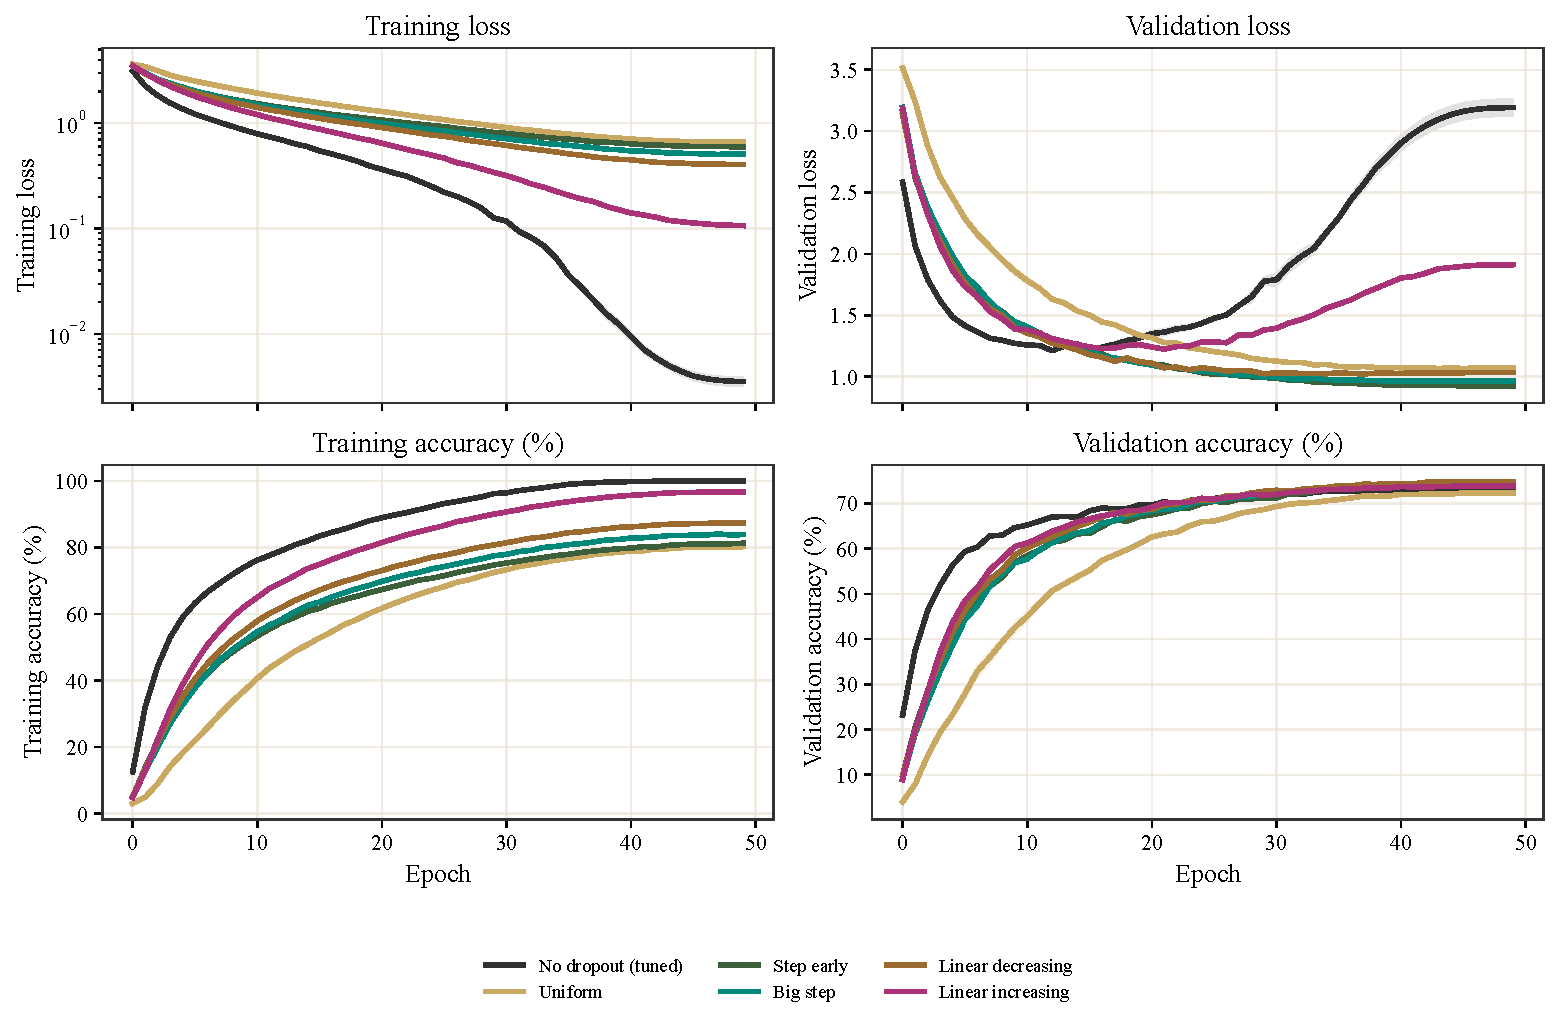
\includegraphics[width=0.92\textwidth]{figures/experiments/benchmarks/speech-commands-mlp.pdf}
\caption{Speech Commands / MLP / Zero weight decay. Original-cohort learning curves; bands show SEM across the recorded seeds for each profile. Sample counts and tuned probabilities are given below.}
\label{fig:speech-commands-mlp}
\end{figure}
\begin{center}\small
\begin{tabular}{@{}lrrrrrr@{}}
\toprule
Profile & $n$ & $\bar p$ & Learning rate & Test CE & Test acc. (\%) & Final test CE \\
\midrule
No dropout (tuned) & 5 & 0.00 & 1e-03 & \(1.203\pm0.011\) & \(67.16\pm0.35\) & -- \\
Uniform & 5 & 0.10 & 1e-03 & \(1.073\pm0.006\) & \(72.23\pm0.12\) & -- \\
Step early & 5 & 0.05 & 1e-03 & \(0.937\pm0.003\) & \(74.06\pm0.13\) & -- \\
Big step & 5 & 0.05 & 1e-03 & \(0.950\pm0.004\) & \(74.07\pm0.11\) & -- \\
Linear decreasing & 5 & 0.05 & 1e-03 & \(1.002\pm0.005\) & \(73.87\pm0.45\) & -- \\
Linear increasing & 5 & 0.05 & 1e-03 & \(1.202\pm0.009\) & \(69.40\pm0.54\) & -- \\
\bottomrule\end{tabular}\end{center}
\emph{Test endpoints.} Test CE and accuracy use the minimum-validation-loss checkpoint. Dashes indicate that final-epoch test CE was not recorded in this original cohort; the final losses in the learning curves are validation losses.
For the validation-selected nonuniform profile, the paired test-CE difference (profile minus uniform) is \(-0.136\pm0.007\) (SEM).
\clearpage
\subsection{Speech Commands / Transformer / Zero weight decay}
Depth 12, width 256; 20,020/5,005/10,010 training/validation/test examples; 50 epochs, batch size 128, weight decay \(0\). The recorded split is held fixed across profiles.
\begin{figure}[ht]
\centering
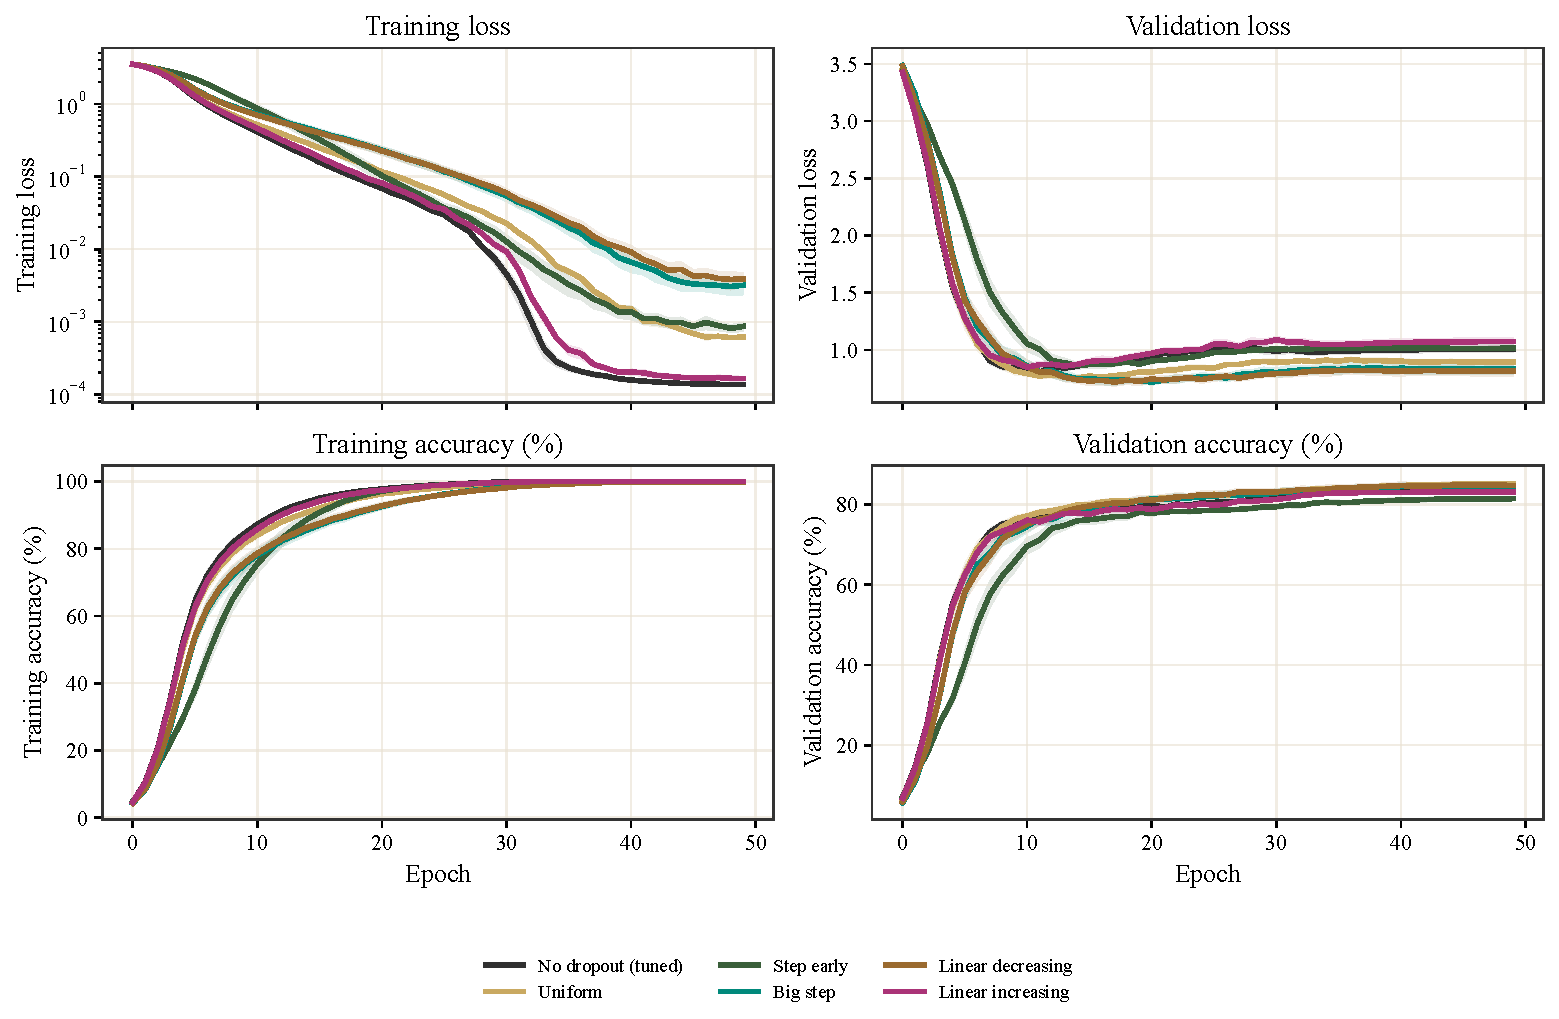
\includegraphics[width=0.92\textwidth]{figures/experiments/benchmarks/speech-commands-transformer.pdf}
\caption{Speech Commands / Transformer / Zero weight decay. Original-cohort learning curves; bands show SEM across the recorded seeds for each profile. Sample counts and tuned probabilities are given below.}
\label{fig:speech-commands-transformer}
\end{figure}
\begin{center}\small
\begin{tabular}{@{}lrrrrrr@{}}
\toprule
Profile & $n$ & $\bar p$ & Learning rate & Test CE & Test acc. (\%) & Final test CE \\
\midrule
No dropout (tuned) & 5 & 0.00 & 3e-04 & \(0.807\pm0.018\) & \(77.65\pm0.65\) & -- \\
Uniform & 5 & 0.15 & 3e-04 & \(0.743\pm0.017\) & \(79.54\pm0.61\) & -- \\
Step early & 5 & 0.05 & 1e-04 & \(0.852\pm0.027\) & \(77.85\pm0.64\) & -- \\
Big step & 5 & 0.15 & 3e-04 & \(0.707\pm0.036\) & \(81.07\pm0.89\) & -- \\
Linear decreasing & 5 & 0.20 & 3e-04 & \(0.711\pm0.033\) & \(81.27\pm1.05\) & -- \\
Linear increasing & 5 & 0.10 & 3e-04 & \(0.832\pm0.022\) & \(77.67\pm0.67\) & -- \\
\bottomrule\end{tabular}\end{center}
\emph{Test endpoints.} Test CE and accuracy use the minimum-validation-loss checkpoint. Dashes indicate that final-epoch test CE was not recorded in this original cohort; the final losses in the learning curves are validation losses.
For the validation-selected nonuniform profile, the paired test-CE difference (profile minus uniform) is \(-0.036\pm0.037\) (SEM).
\clearpage
\subsection{Tiny ImageNet / MLP / 80,000 train}
Depth 12, width 256; 80,000/10,000/10,000 training/validation/test examples; 75 epochs, batch size 128, weight decay \(0\). The recorded split is held fixed across profiles.
\begin{figure}[ht]
\centering
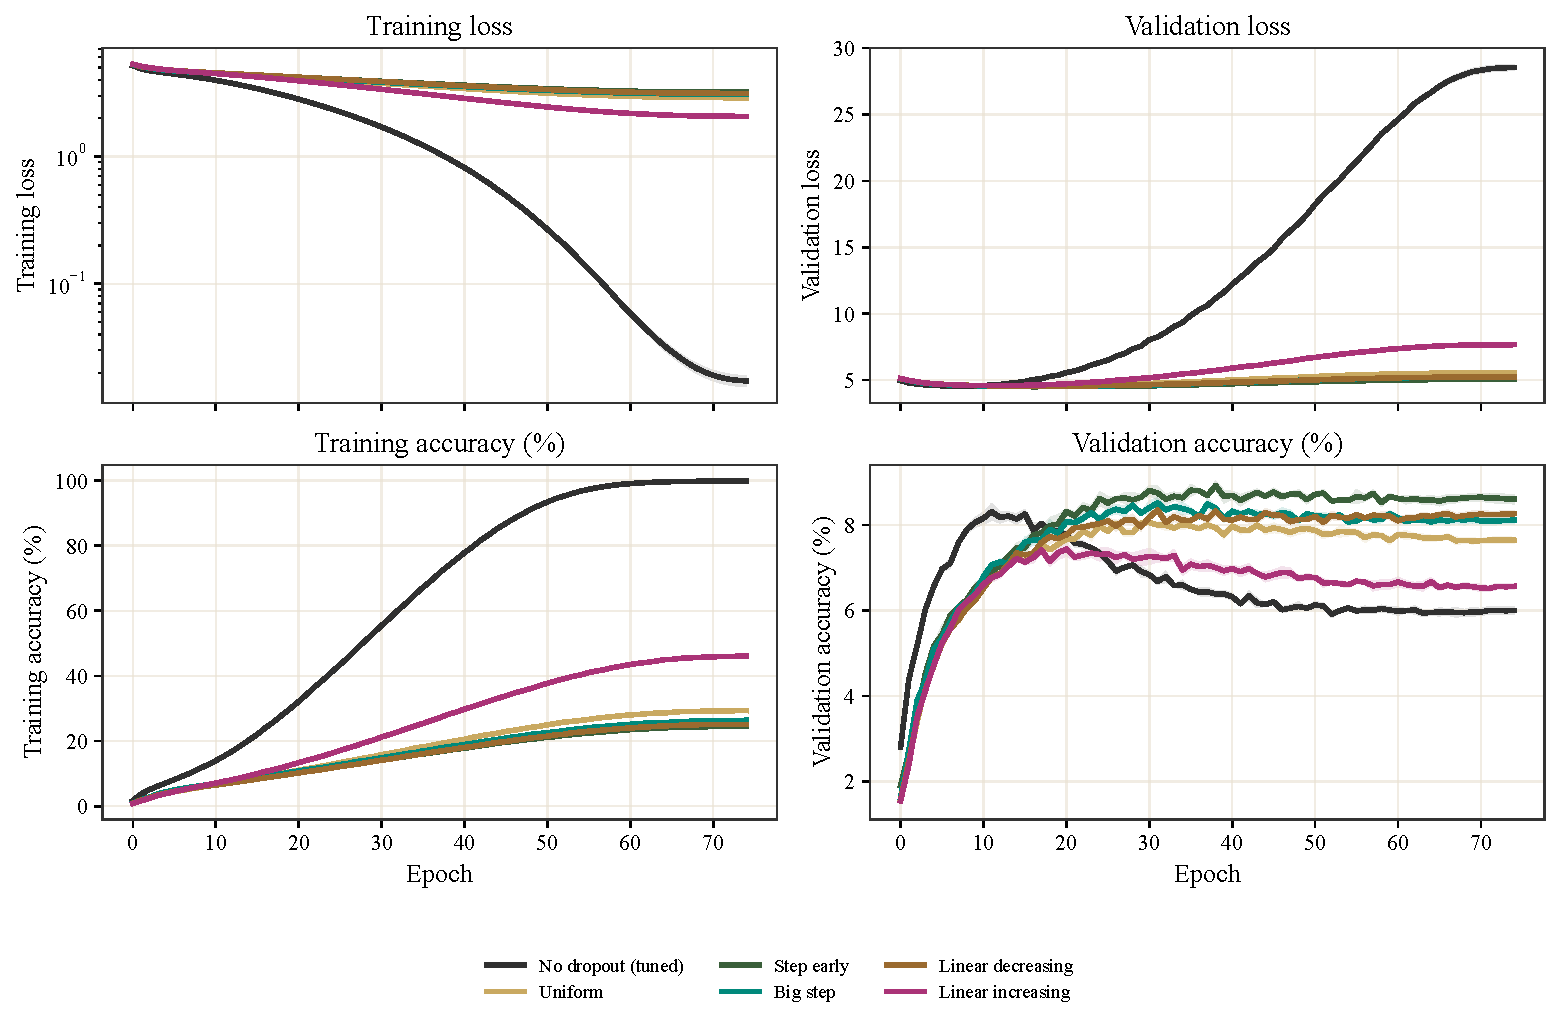
\includegraphics[width=0.92\textwidth]{figures/experiments/benchmarks/tiny-imagenet-mlp-80k.pdf}
\caption{Tiny ImageNet / MLP / 80,000 train. Original-cohort learning curves; bands show SEM across the recorded seeds for each profile. Sample counts and tuned probabilities are given below.}
\label{fig:tiny-imagenet-mlp-80k}
\end{figure}
\begin{center}\small
\begin{tabular}{@{}lrrrrrr@{}}
\toprule
Profile & $n$ & $\bar p$ & Learning rate & Test CE & Test acc. (\%) & Final test CE \\
\midrule
No dropout (tuned) & 5 & 0.00 & 3e-04 & \(4.561\pm0.004\) & \(7.64\pm0.15\) & \(28.876\pm0.230\) \\
Uniform & 5 & 0.05 & 3e-04 & \(4.575\pm0.002\) & \(7.09\pm0.14\) & \(5.627\pm0.004\) \\
Step early & 5 & 0.05 & 3e-04 & \(4.518\pm0.004\) & \(7.95\pm0.10\) & \(5.130\pm0.009\) \\
Big step & 5 & 0.05 & 3e-04 & \(4.541\pm0.003\) & \(7.53\pm0.12\) & \(5.321\pm0.007\) \\
Linear decreasing & 5 & 0.05 & 3e-04 & \(4.563\pm0.003\) & \(7.19\pm0.15\) & \(5.286\pm0.013\) \\
Linear increasing & 5 & 0.05 & 3e-04 & \(4.608\pm0.005\) & \(6.75\pm0.12\) & \(7.764\pm0.023\) \\
\bottomrule\end{tabular}\end{center}
For the validation-selected nonuniform profile, the paired test-CE difference (profile minus uniform) is \(-0.058\pm0.005\) (SEM).
\clearpage
\subsection{Tiny ImageNet / Transformer / 80,000 train}
Depth 12, width 256; 80,000/10,000/10,000 training/validation/test examples; 75 epochs, batch size 128, weight decay \(0\). The recorded split is held fixed across profiles.
\begin{figure}[ht]
\centering
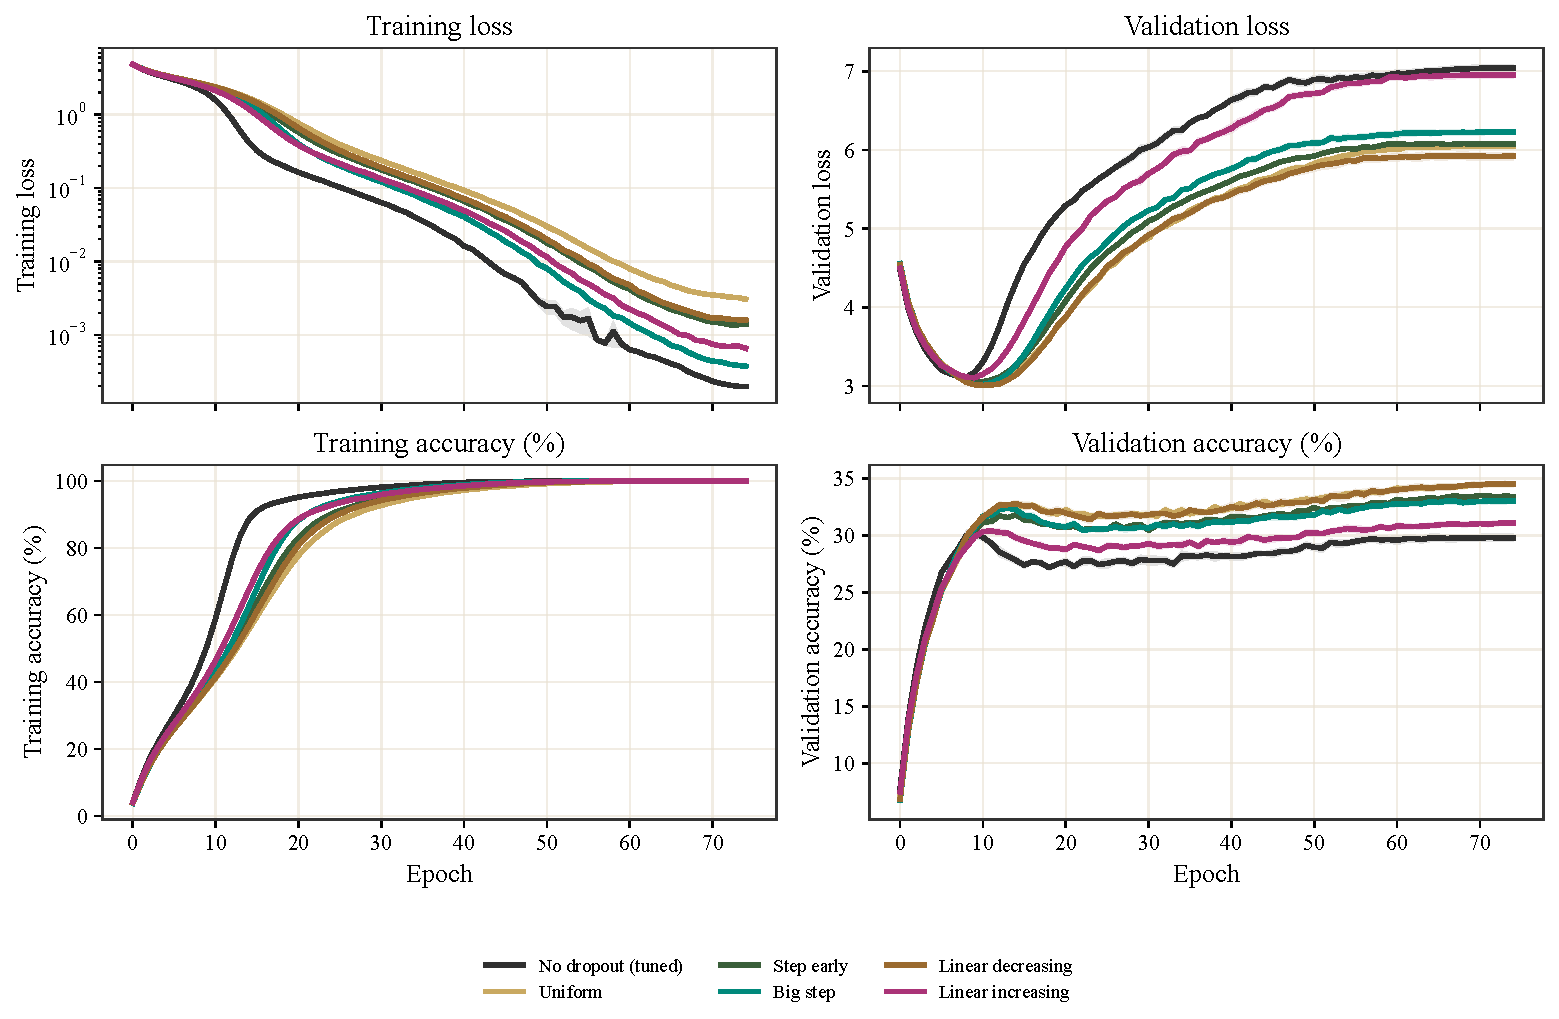
\includegraphics[width=0.92\textwidth]{figures/experiments/benchmarks/tiny-imagenet-transformer-80k.pdf}
\caption{Tiny ImageNet / Transformer / 80,000 train. Original-cohort learning curves; bands show SEM across the recorded seeds for each profile. Sample counts and tuned probabilities are given below.}
\label{fig:tiny-imagenet-transformer-80k}
\end{figure}
\begin{center}\small
\begin{tabular}{@{}lrrrrrr@{}}
\toprule
Profile & $n$ & $\bar p$ & Learning rate & Test CE & Test acc. (\%) & Final test CE \\
\midrule
No dropout (tuned) & 5 & 0.00 & 3e-04 & \(3.125\pm0.025\) & \(29.57\pm0.44\) & \(7.126\pm0.068\) \\
Uniform & 5 & 0.20 & 3e-04 & \(3.035\pm0.014\) & \(31.49\pm0.17\) & \(6.104\pm0.043\) \\
Step early & 5 & 0.15 & 3e-04 & \(3.053\pm0.015\) & \(31.22\pm0.21\) & \(6.164\pm0.025\) \\
Big step & 5 & 0.10 & 3e-04 & \(3.026\pm0.013\) & \(31.35\pm0.38\) & \(6.296\pm0.034\) \\
Linear decreasing & 5 & 0.15 & 3e-04 & \(3.004\pm0.016\) & \(31.78\pm0.23\) & \(6.002\pm0.042\) \\
Linear increasing & 5 & 0.20 & 3e-04 & \(3.118\pm0.017\) & \(29.72\pm0.26\) & \(7.026\pm0.052\) \\
\bottomrule\end{tabular}\end{center}
For the validation-selected nonuniform profile, the paired test-CE difference (profile minus uniform) is \(-0.031\pm0.015\) (SEM).
\clearpage
\subsection{FI-2010 / Transformer / Linear follow-up}
Depth 12, width 256; 40,000/10,000/20,000 training/validation/test examples; 50 epochs, batch size 128, weight decay \(1e-07\). The recorded split is held fixed across profiles.
\begin{figure}[ht]
\centering
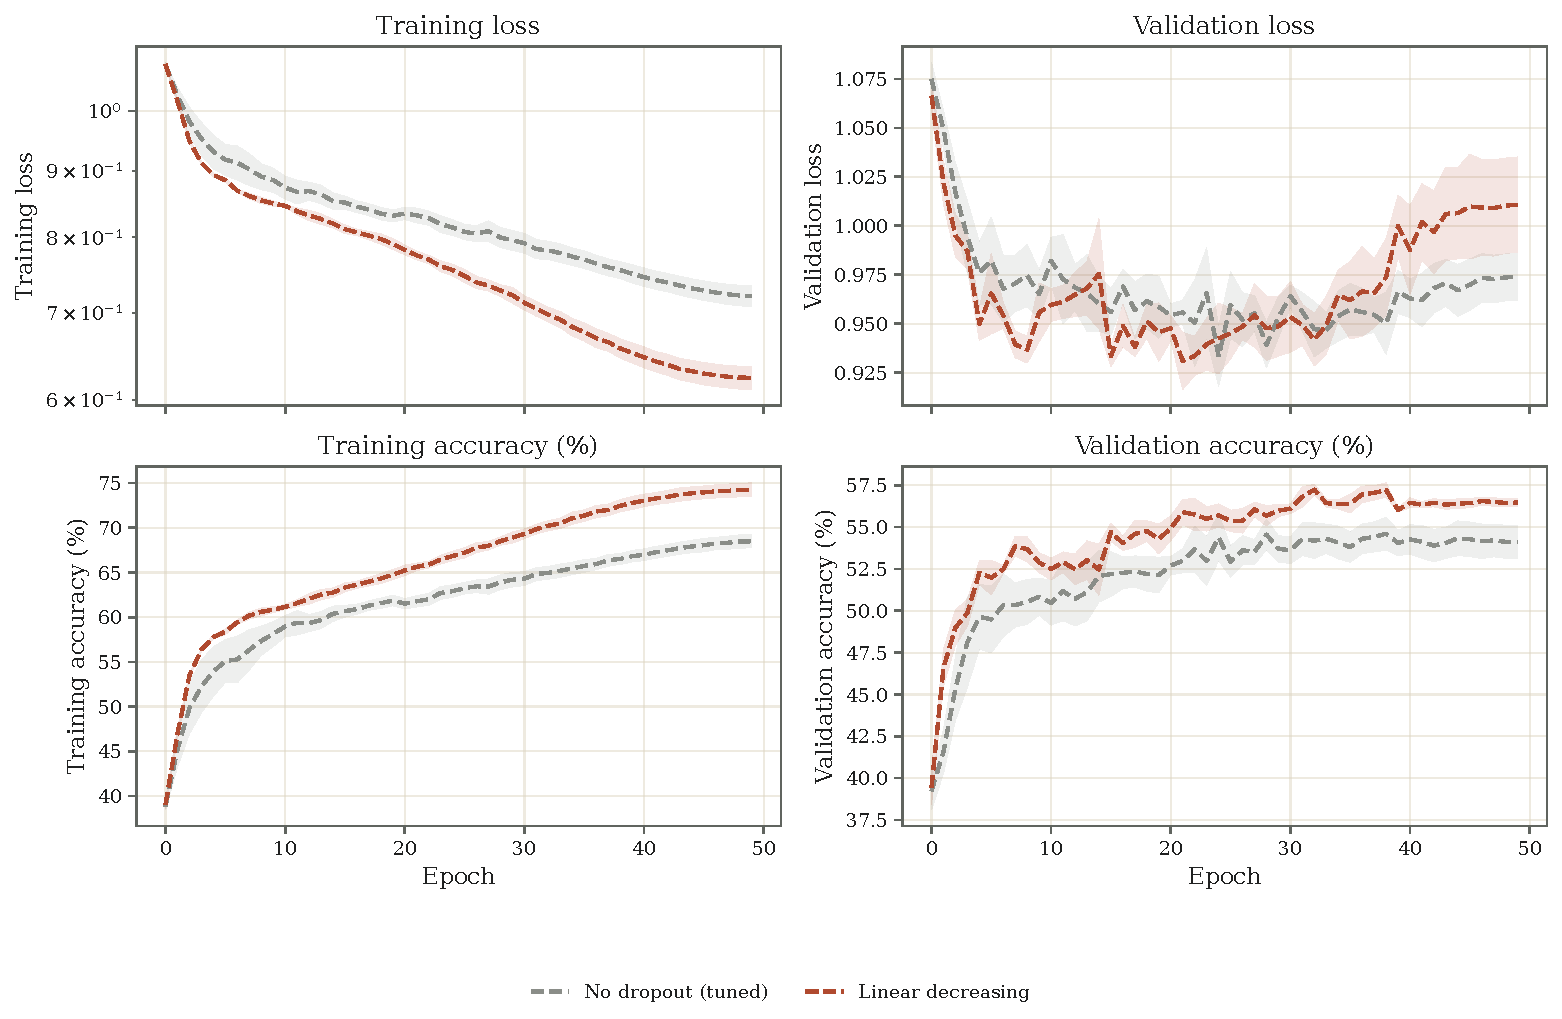
\includegraphics[width=0.92\textwidth]{figures/experiments/benchmarks/fi2010-transformer-linear.pdf}
\caption{FI-2010 / Transformer / Linear follow-up. Original-cohort learning curves; bands show SEM across the recorded seeds for each profile. Sample counts and tuned probabilities are given below.}
\label{fig:fi2010-transformer-linear}
\end{figure}
\begin{center}\small
\begin{tabular}{@{}lrrrrrr@{}}
\toprule
Profile & $n$ & $\bar p$ & Learning rate & Test CE & Test acc. (\%) & Final test CE \\
\midrule
No dropout (tuned) & 5 & 0.00 & 1e-03 & \(0.955\pm0.010\) & \(55.38\pm0.39\) & -- \\
Linear decreasing & 5 & 0.10 & 1e-03 & \(0.930\pm0.006\) & \(57.72\pm0.83\) & -- \\
\bottomrule\end{tabular}\end{center}
\clearpage
\subsection{Jannis / Transformer / Linear follow-up}
Depth 12, width 256; 3,840/960/1,920 training/validation/test examples; 50 epochs, batch size 128, weight decay \(1e-07\). The recorded split is held fixed across profiles.
\begin{figure}[ht]
\centering
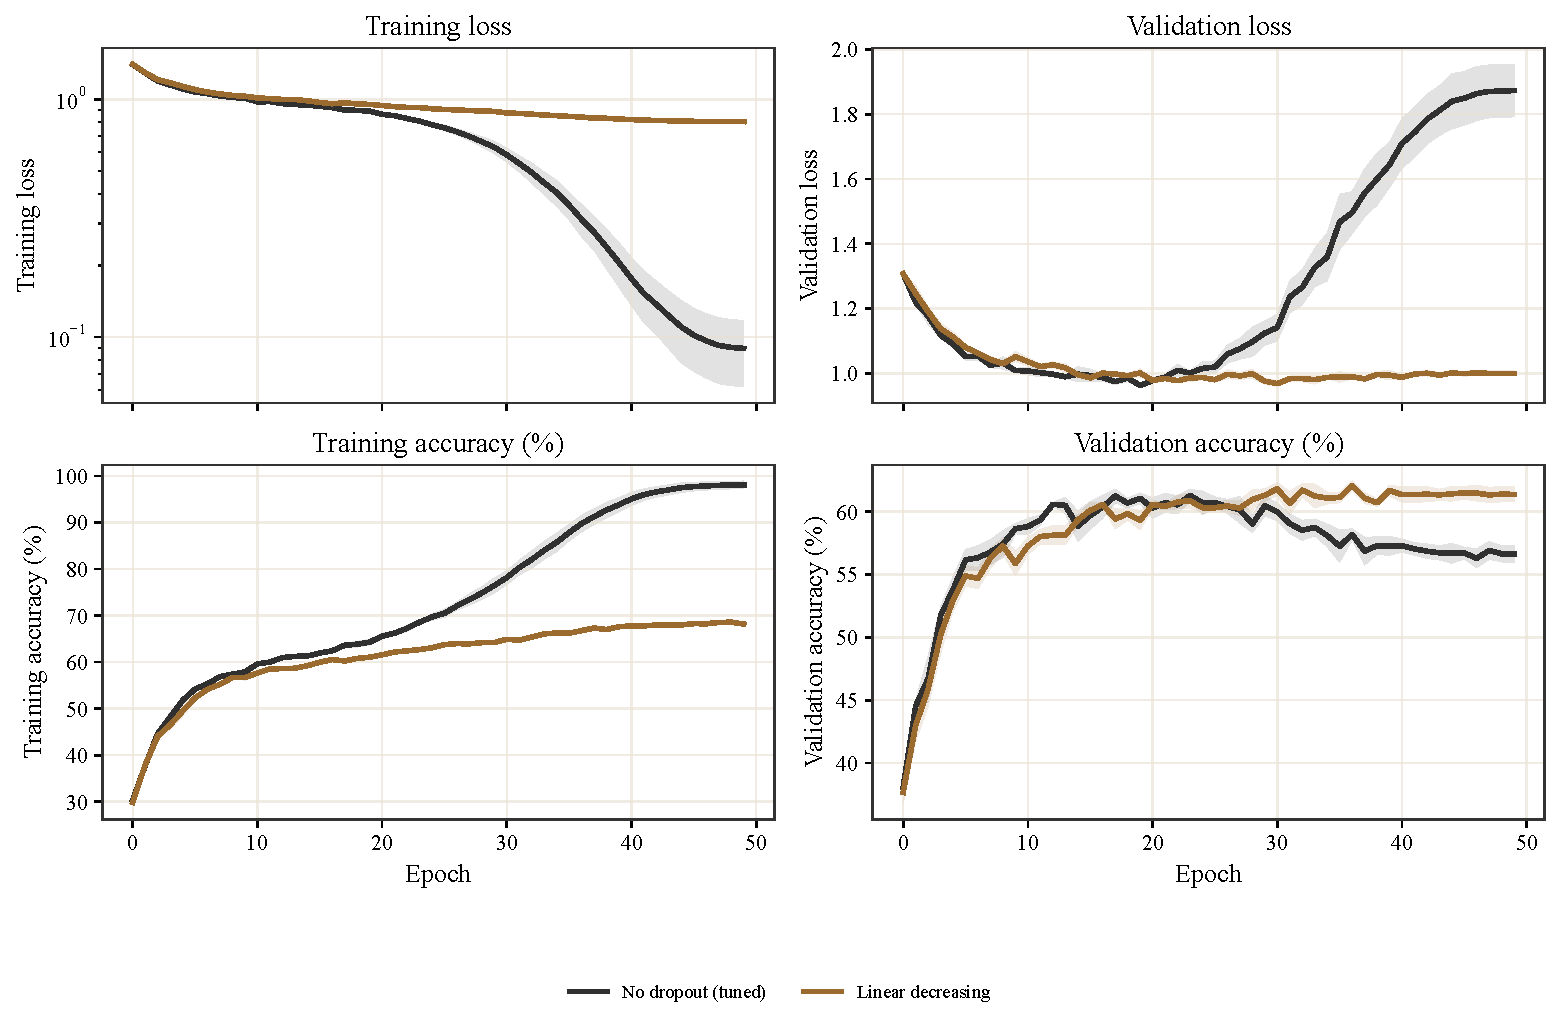
\includegraphics[width=0.92\textwidth]{figures/experiments/benchmarks/jannis-transformer-linear.pdf}
\caption{Jannis / Transformer / Linear follow-up. Original-cohort learning curves; bands show SEM across the recorded seeds for each profile. Sample counts and tuned probabilities are given below.}
\label{fig:jannis-transformer-linear}
\end{figure}
\begin{center}\small
\begin{tabular}{@{}lrrrrrr@{}}
\toprule
Profile & $n$ & $\bar p$ & Learning rate & Test CE & Test acc. (\%) & Final test CE \\
\midrule
No dropout (tuned) & 5 & 0.00 & 1e-04 & \(0.986\pm0.002\) & \(59.07\pm0.47\) & -- \\
Linear decreasing & 5 & 0.10 & 1e-04 & \(0.992\pm0.005\) & \(60.27\pm0.43\) & -- \\
\bottomrule\end{tabular}\end{center}
\clearpage
\subsection{Jannis / Transformer / 100 epochs}
Depth 12, width 256; 3,840/960/1,920 training/validation/test examples; 100 epochs, batch size 128, weight decay \(1e-07\). The recorded split is held fixed across profiles.
\begin{figure}[ht]
\centering
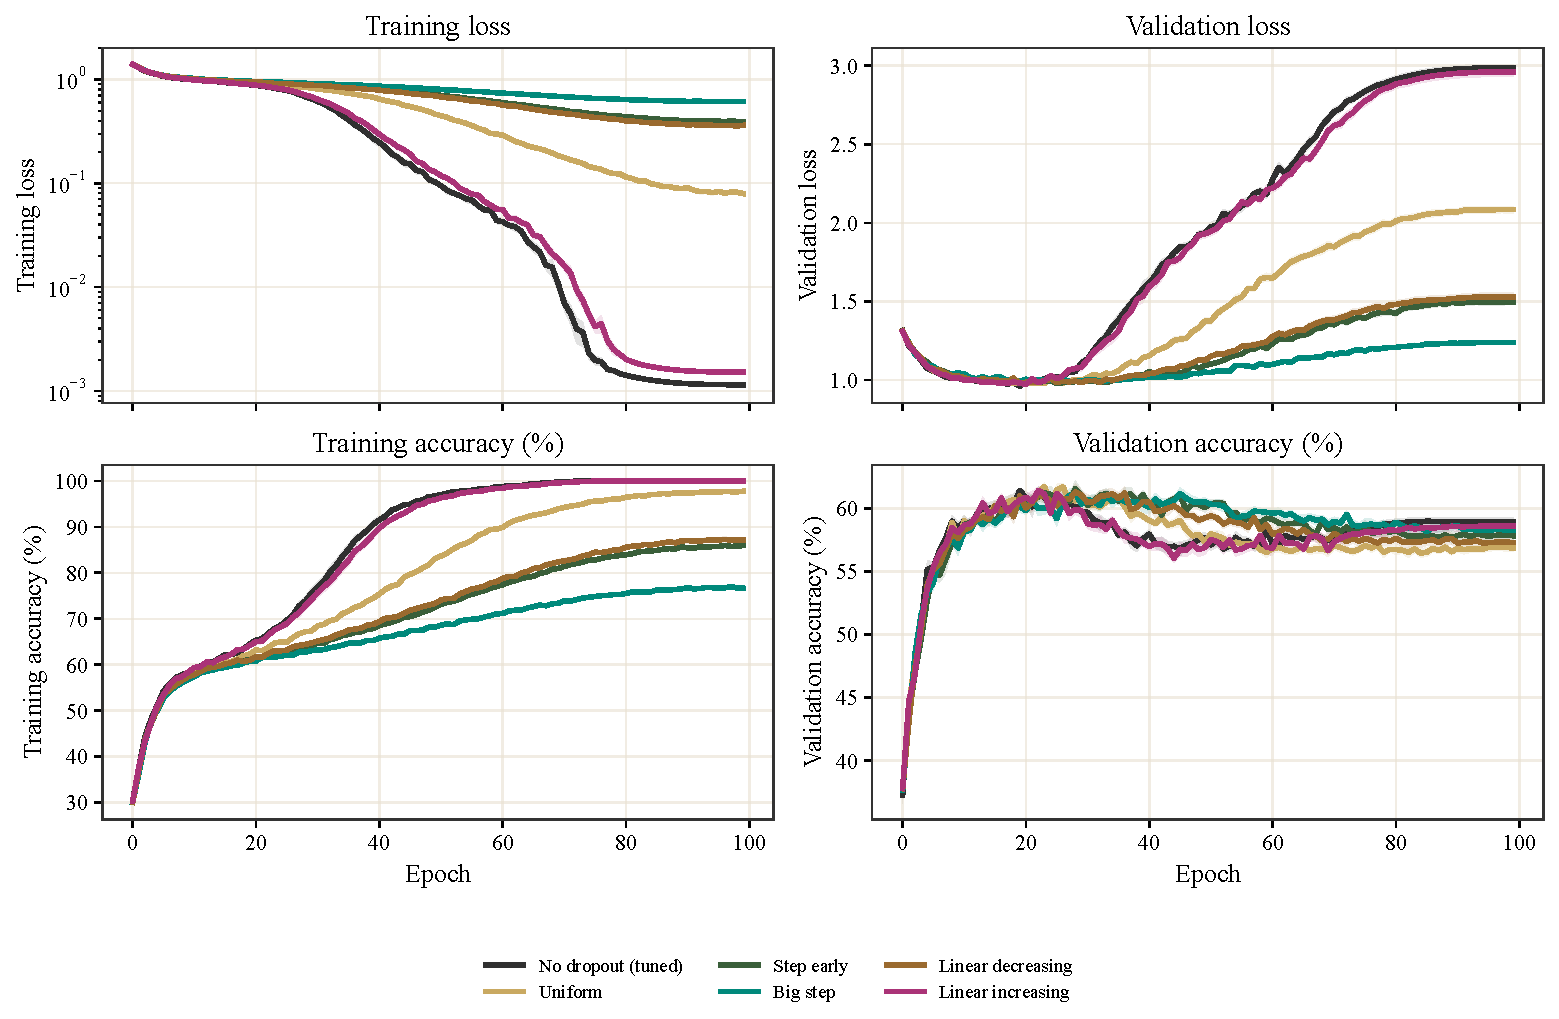
\includegraphics[width=0.92\textwidth]{figures/experiments/benchmarks/jannis-transformer-100-epochs.pdf}
\caption{Jannis / Transformer / 100 epochs. Original-cohort learning curves; bands show SEM across the recorded seeds for each profile. Sample counts and tuned probabilities are given below.}
\label{fig:jannis-transformer-100-epochs}
\end{figure}
\begin{center}\small
\begin{tabular}{@{}lrrrrrr@{}}
\toprule
Profile & $n$ & $\bar p$ & Learning rate & Test CE & Test acc. (\%) & Final test CE \\
\midrule
No dropout (tuned) & 10 & 0.00 & 1e-04 & \(0.985\pm0.003\) & \(59.54\pm0.16\) & -- \\
Uniform & 10 & 0.10 & 1e-04 & \(0.988\pm0.002\) & \(59.46\pm0.23\) & -- \\
Step early & 10 & 0.10 & 1e-04 & \(0.990\pm0.004\) & \(59.85\pm0.21\) & -- \\
Big step & 10 & 0.10 & 1e-04 & \(0.999\pm0.003\) & \(59.36\pm0.29\) & -- \\
Linear decreasing & 10 & 0.10 & 1e-04 & \(0.988\pm0.003\) & \(59.75\pm0.13\) & -- \\
Linear increasing & 10 & 0.10 & 1e-04 & \(0.992\pm0.003\) & \(59.40\pm0.25\) & -- \\
\bottomrule\end{tabular}\end{center}
For the validation-selected nonuniform profile, the paired test-CE difference (profile minus uniform) is \(0.004\pm0.003\) (SEM).
\clearpage
\subsection{Tiny ImageNet / MLP / Zero weight decay}
Depth 12, width 256; 20,000/5,000/10,000 training/validation/test examples; 75 epochs, batch size 128, weight decay \(0\). The recorded split is held fixed across profiles.
\begin{figure}[ht]
\centering
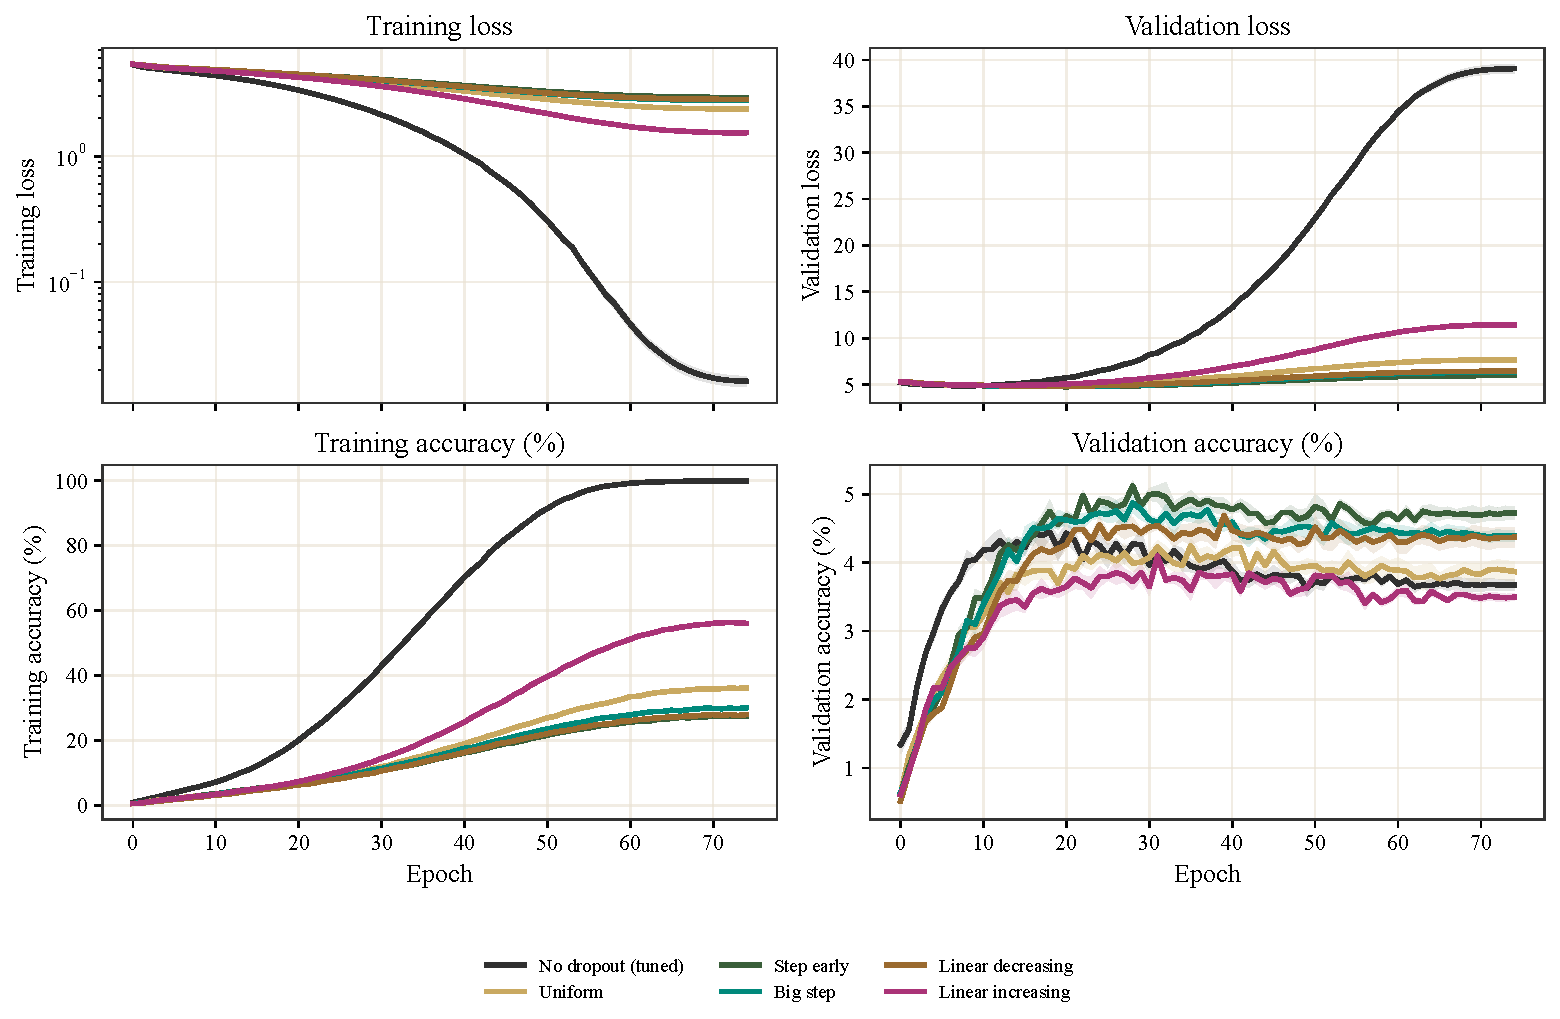
\includegraphics[width=0.92\textwidth]{figures/experiments/benchmarks/tiny-imagenet-mlp-20k.pdf}
\caption{Tiny ImageNet / MLP / Zero weight decay. Original-cohort learning curves; bands show SEM across the recorded seeds for each profile. Sample counts and tuned probabilities are given below.}
\label{fig:tiny-imagenet-mlp-20k}
\end{figure}
\begin{center}\small
\begin{tabular}{@{}lrrrrrr@{}}
\toprule
Profile & $n$ & $\bar p$ & Learning rate & Test CE & Test acc. (\%) & Final test CE \\
\midrule
No dropout (tuned) & 5 & 0.00 & 1e-03 & \(4.856\pm0.005\) & \(3.88\pm0.05\) & -- \\
Uniform & 5 & 0.05 & 1e-03 & \(4.868\pm0.006\) & \(3.45\pm0.06\) & -- \\
Step early & 5 & 0.05 & 3e-04 & \(4.774\pm0.006\) & \(4.84\pm0.04\) & -- \\
Big step & 5 & 0.05 & 3e-04 & \(4.787\pm0.003\) & \(4.61\pm0.10\) & -- \\
Linear decreasing & 5 & 0.05 & 3e-04 & \(4.823\pm0.004\) & \(4.38\pm0.10\) & -- \\
Linear increasing & 5 & 0.05 & 1e-03 & \(4.898\pm0.007\) & \(3.36\pm0.09\) & -- \\
\bottomrule\end{tabular}\end{center}
For the validation-selected nonuniform profile, the paired test-CE difference (profile minus uniform) is \(-0.094\pm0.011\) (SEM).
\clearpage
\subsection{Tiny ImageNet / Transformer / Zero weight decay}
Depth 12, width 256; 20,000/5,000/10,000 training/validation/test examples; 75 epochs, batch size 128, weight decay \(0\). The recorded split is held fixed across profiles.
\begin{figure}[ht]
\centering
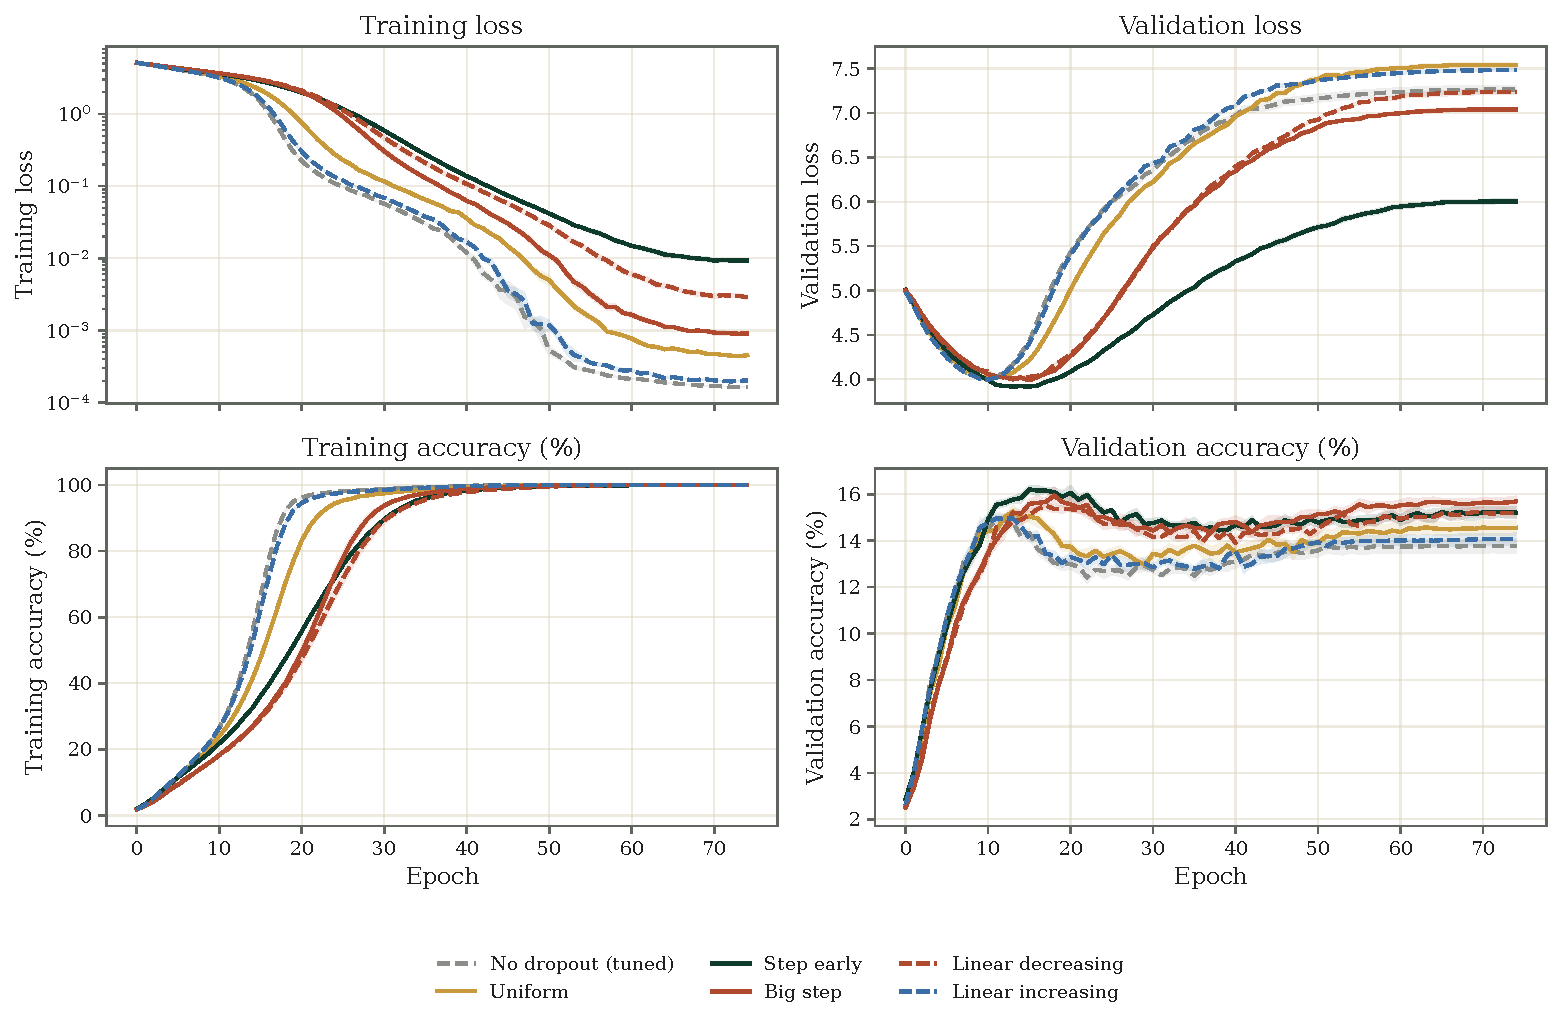
\includegraphics[width=0.92\textwidth]{figures/experiments/benchmarks/tiny-imagenet-transformer-20k.pdf}
\caption{Tiny ImageNet / Transformer / Zero weight decay. Original-cohort learning curves; bands show SEM across the recorded seeds for each profile. Sample counts and tuned probabilities are given below.}
\label{fig:tiny-imagenet-transformer-20k}
\end{figure}
\begin{center}\small
\begin{tabular}{@{}lrrrrrr@{}}
\toprule
Profile & $n$ & $\bar p$ & Learning rate & Test CE & Test acc. (\%) & Final test CE \\
\midrule
No dropout (tuned) & 5 & 0.00 & 3e-04 & \(3.981\pm0.012\) & \(14.92\pm0.21\) & -- \\
Uniform & 5 & 0.10 & 3e-04 & \(3.976\pm0.007\) & \(14.63\pm0.17\) & -- \\
Step early & 5 & 0.15 & 1e-04 & \(3.890\pm0.008\) & \(16.26\pm0.10\) & -- \\
Big step & 5 & 0.15 & 3e-04 & \(3.960\pm0.012\) & \(15.45\pm0.29\) & -- \\
Linear decreasing & 5 & 0.20 & 3e-04 & \(3.980\pm0.011\) & \(14.71\pm0.22\) & -- \\
Linear increasing & 5 & 0.05 & 3e-04 & \(3.981\pm0.017\) & \(14.73\pm0.30\) & -- \\
\bottomrule\end{tabular}\end{center}
For the validation-selected nonuniform profile, the paired test-CE difference (profile minus uniform) is \(-0.086\pm0.013\) (SEM).
\clearpage
\subsection{FI-2010 / MLP / Zero weight decay}
Depth 12, width 256; 40,000/10,000/20,000 training/validation/test examples; 50 epochs, batch size 128, weight decay \(0\). The recorded split is held fixed across profiles.
\begin{figure}[ht]
\centering
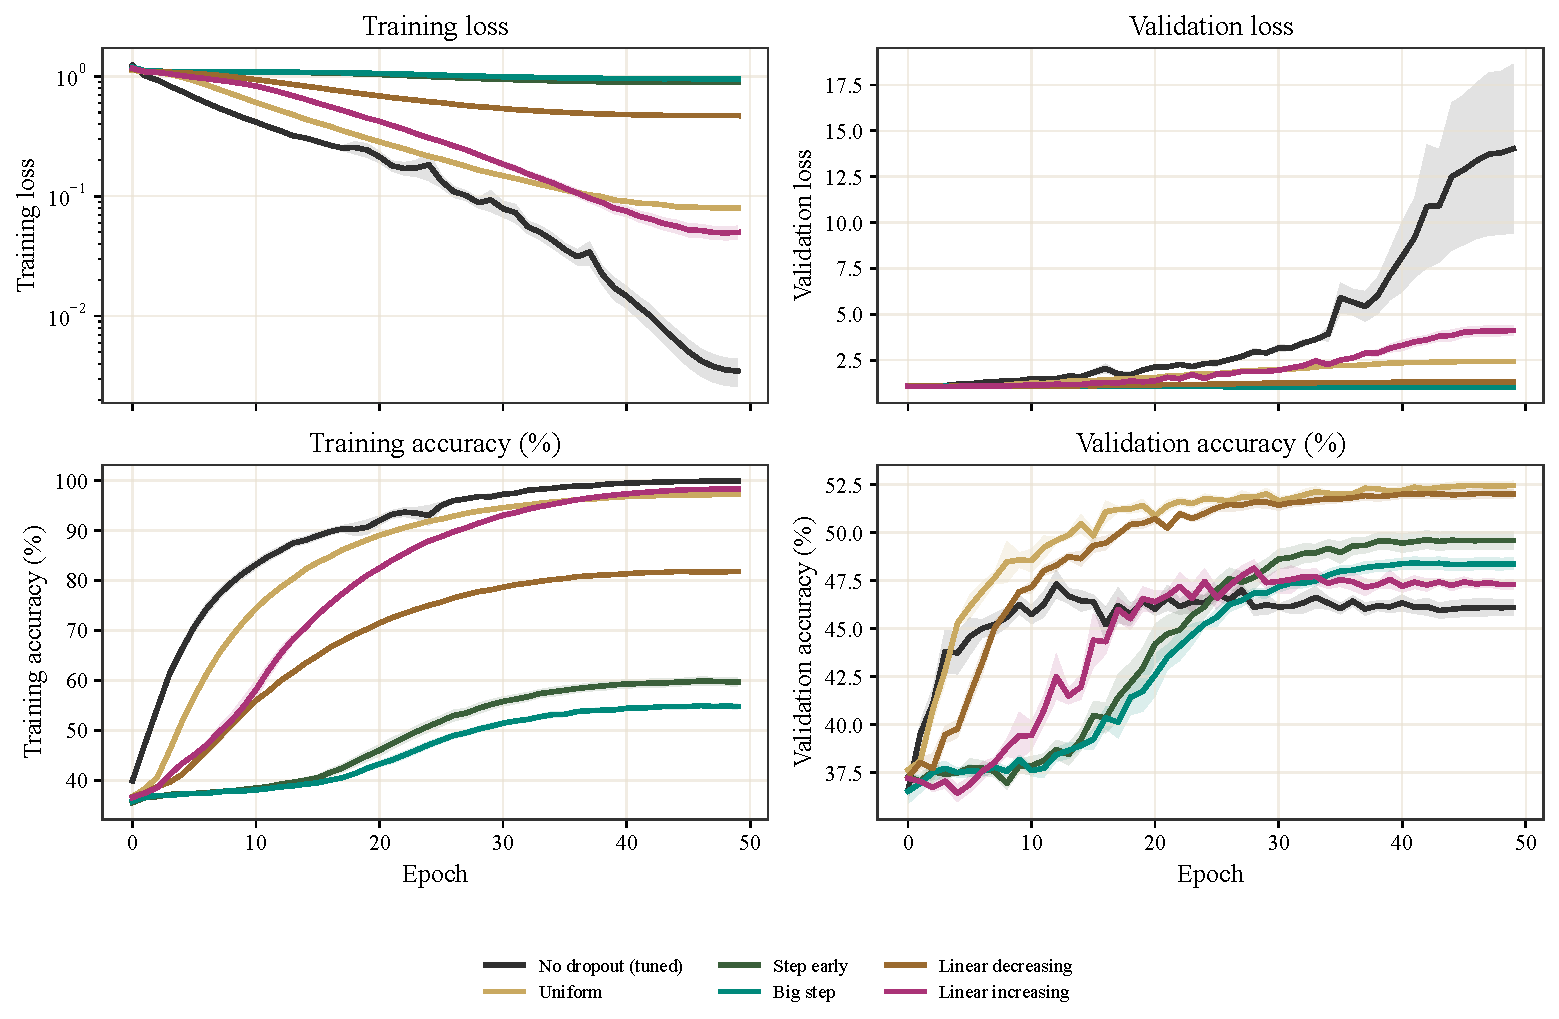
\includegraphics[width=0.92\textwidth]{figures/experiments/benchmarks/fi2010-mlp.pdf}
\caption{FI-2010 / MLP / Zero weight decay. Original-cohort learning curves; bands show SEM across the recorded seeds for each profile. Sample counts and tuned probabilities are given below.}
\label{fig:fi2010-mlp}
\end{figure}
\begin{center}\small
\begin{tabular}{@{}lrrrrrr@{}}
\toprule
Profile & $n$ & $\bar p$ & Learning rate & Test CE & Test acc. (\%) & Final test CE \\
\midrule
No dropout (tuned) & 5 & 0.00 & 3e-03 & \(1.118\pm0.017\) & \(42.19\pm2.20\) & -- \\
Uniform & 5 & 0.05 & 1e-04 & \(1.093\pm0.004\) & \(47.70\pm0.37\) & -- \\
Step early & 5 & 0.10 & 3e-05 & \(1.061\pm0.004\) & \(48.19\pm0.33\) & -- \\
Big step & 5 & 0.10 & 3e-05 & \(1.054\pm0.004\) & \(48.37\pm0.39\) & -- \\
Linear decreasing & 5 & 0.05 & 3e-05 & \(1.074\pm0.008\) & \(47.48\pm0.27\) & -- \\
Linear increasing & 5 & 0.15 & 1e-03 & \(1.115\pm0.011\) & \(37.62\pm0.39\) & -- \\
\bottomrule\end{tabular}\end{center}
For the validation-selected nonuniform profile, the paired test-CE difference (profile minus uniform) is \(-0.039\pm0.005\) (SEM).
\clearpage
\subsection{Jannis / MLP / Zero weight decay}
Depth 12, width 256; 3,840/960/1,920 training/validation/test examples; 100 epochs, batch size 128, weight decay \(0\). The recorded split is held fixed across profiles.
\begin{figure}[ht]
\centering
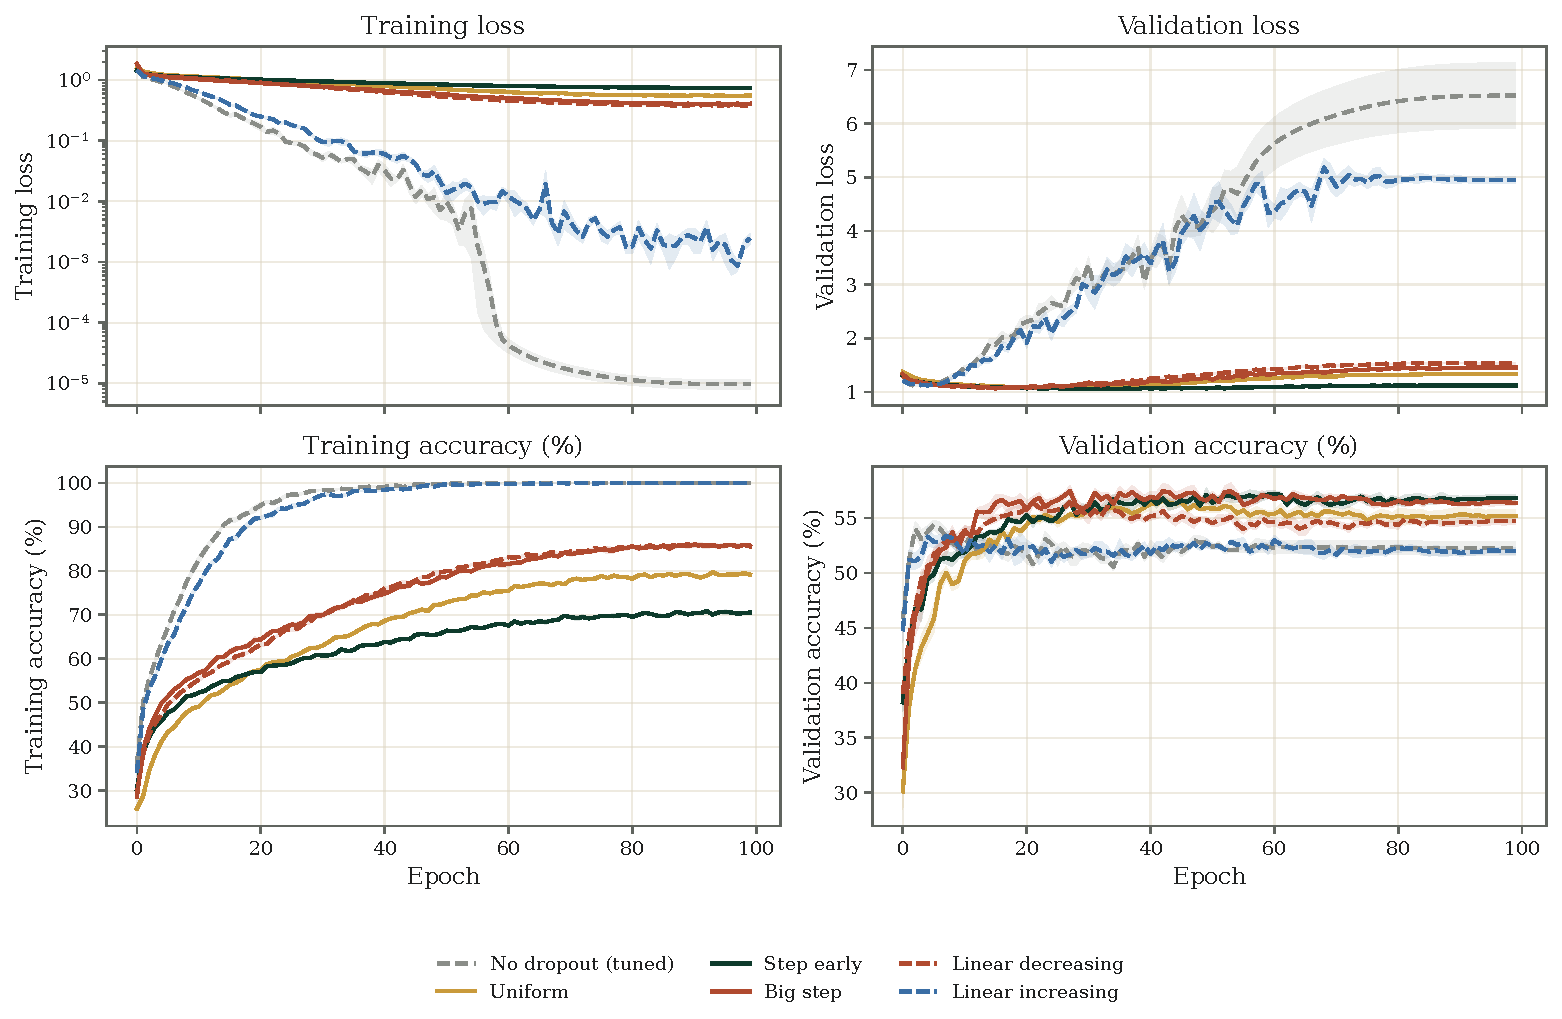
\includegraphics[width=0.92\textwidth]{figures/experiments/benchmarks/jannis-mlp.pdf}
\caption{Jannis / MLP / Zero weight decay. Original-cohort learning curves; bands show SEM across the recorded seeds for each profile. Sample counts and tuned probabilities are given below.}
\label{fig:jannis-mlp}
\end{figure}
\begin{center}\small
\begin{tabular}{@{}lrrrrrr@{}}
\toprule
Profile & $n$ & $\bar p$ & Learning rate & Test CE & Test acc. (\%) & Final test CE \\
\midrule
No dropout (tuned) & 5 & 0.00 & 3e-03 & \(1.123\pm0.006\) & \(51.56\pm0.38\) & -- \\
Uniform & 5 & 0.10 & 3e-04 & \(1.123\pm0.007\) & \(52.96\pm0.20\) & -- \\
Step early & 5 & 0.05 & 3e-04 & \(1.091\pm0.004\) & \(54.25\pm0.41\) & -- \\
Big step & 5 & 0.10 & 3e-03 & \(1.087\pm0.003\) & \(55.00\pm0.43\) & -- \\
Linear decreasing & 5 & 0.05 & 3e-04 & \(1.110\pm0.004\) & \(53.18\pm0.52\) & -- \\
Linear increasing & 5 & 0.05 & 3e-03 & \(1.140\pm0.008\) & \(51.77\pm0.71\) & -- \\
\bottomrule\end{tabular}\end{center}
For the validation-selected nonuniform profile, the paired test-CE difference (profile minus uniform) is \(-0.033\pm0.010\) (SEM).
\clearpage
\subsection{Jannis / Transformer / Zero weight decay}
Depth 12, width 256; 3,840/960/1,920 training/validation/test examples; 100 epochs, batch size 128, weight decay \(0\). The recorded split is held fixed across profiles.
\begin{figure}[ht]
\centering
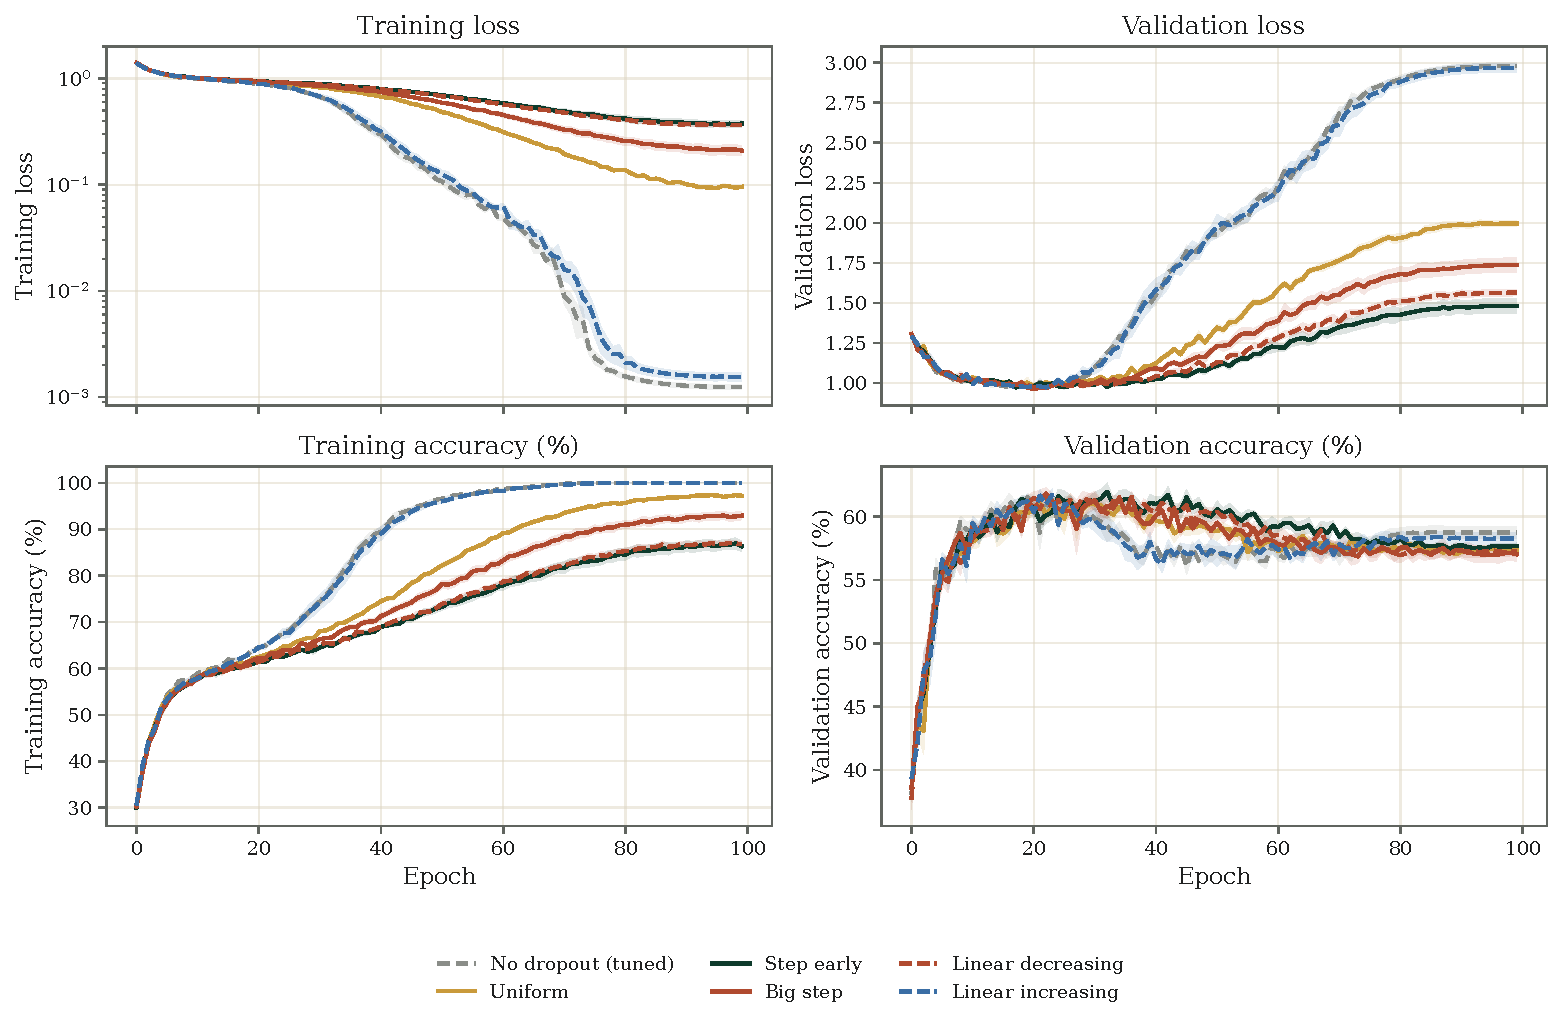
\includegraphics[width=0.92\textwidth]{figures/experiments/benchmarks/jannis-transformer.pdf}
\caption{Jannis / Transformer / Zero weight decay. Original-cohort learning curves; bands show SEM across the recorded seeds for each profile. Sample counts and tuned probabilities are given below.}
\label{fig:jannis-transformer}
\end{figure}
\begin{center}\small
\begin{tabular}{@{}lrrrrrr@{}}
\toprule
Profile & $n$ & $\bar p$ & Learning rate & Test CE & Test acc. (\%) & Final test CE \\
\midrule
No dropout (tuned) & 5 & 0.00 & 1e-04 & \(0.985\pm0.002\) & \(59.50\pm0.10\) & -- \\
Uniform & 5 & 0.10 & 1e-04 & \(0.993\pm0.004\) & \(58.98\pm0.19\) & -- \\
Step early & 5 & 0.05 & 1e-04 & \(0.988\pm0.001\) & \(59.22\pm0.21\) & -- \\
Big step & 5 & 0.05 & 1e-04 & \(0.992\pm0.003\) & \(59.24\pm0.57\) & -- \\
Linear decreasing & 5 & 0.10 & 1e-04 & \(0.994\pm0.003\) & \(58.90\pm0.32\) & -- \\
Linear increasing & 5 & 0.10 & 1e-04 & \(0.988\pm0.003\) & \(60.28\pm0.26\) & -- \\
\bottomrule\end{tabular}\end{center}
For the validation-selected nonuniform profile, the paired test-CE difference (profile minus uniform) is \(-0.002\pm0.005\) (SEM).
\clearpage
\subsection{Standalone FI-2010 vanilla MLPs}
These plain feedforward ReLU MLPs flatten a $128\times40$ input window. The study uses day 6 for training, day 7 for validation, and days 8--10 for test. Each architecture is trained for 100 epochs with five paired confirmation seeds (100--104), zero weight decay, and mean dropout $0.10$ for nonzero profiles. Weights have variance $1.98/\mathrm{fan\_in}$ and biases variance $0.02$. The learning rate is chosen using uniform-dropout validation runs and then held fixed across profiles, including no dropout. These are separate from the depth-12 width-256 benchmark cohorts.
Test loss, accuracy, and macro-F1 are evaluated once, at the minimum-validation-loss checkpoint. The saved results contain profile means and SEMs, but no validation objectives, per-seed test metrics, or per-epoch test histories. Final-epoch and minimum-over-training test losses are therefore unavailable. The standalone rows in Table~\ref{tab:benchmark_results} retain the retrospective choice of the nonuniform profile with the lowest observed mean checkpoint test CE and use that same profile for accuracy. These rows are separate from the validation-selected benchmark comparisons.
\paragraph{Depth 6, width 256.}
\begin{center}\small\begin{tabular}{@{}lrrr@{}}\toprule
Profile & Checkpoint test CE & Test accuracy (\%) & Macro-F1 (\%) \\
\midrule
No dropout & \(0.8348\pm0.0071\) & \(69.667\pm0.403\) & \(32.96\pm0.34\) \\
Uniform & \(0.8338\pm0.0035\) & \(70.830\pm0.030\) & \(31.74\pm0.31\) \\
Step early & \(0.8332\pm0.0024\) & \(70.851\pm0.027\) & \(30.25\pm0.97\) \\
Big step & \(0.8279\pm0.0019\) & \(70.839\pm0.010\) & \(30.44\pm1.17\) \\
Linear decreasing & \(0.8312\pm0.0035\) & \(70.851\pm0.011\) & \(28.36\pm0.54\) \\
Linear increasing & \(0.8293\pm0.0026\) & \(70.865\pm0.009\) & \(31.45\pm0.56\) \\
Step late & \(0.8227\pm0.0016\) & \(70.855\pm0.019\) & \(31.97\pm0.45\) \\
\bottomrule\end{tabular}\end{center}
\paragraph{Depth 6, width 512.}
\begin{center}\small\begin{tabular}{@{}lrrr@{}}\toprule
Profile & Checkpoint test CE & Test accuracy (\%) & Macro-F1 (\%) \\
\midrule
No dropout & \(0.8327\pm0.0057\) & \(69.838\pm0.392\) & \(32.63\pm1.27\) \\
Uniform & \(0.8318\pm0.0024\) & \(70.854\pm0.020\) & \(31.27\pm0.70\) \\
Step early & \(0.8341\pm0.0044\) & \(70.851\pm0.023\) & \(31.41\pm1.05\) \\
Big step & \(0.8330\pm0.0042\) & \(70.853\pm0.007\) & \(30.91\pm1.27\) \\
Linear decreasing & \(0.8267\pm0.0071\) & \(70.865\pm0.029\) & \(31.15\pm0.81\) \\
Linear increasing & \(0.8342\pm0.0037\) & \(70.866\pm0.005\) & \(31.17\pm0.87\) \\
Step late & \(0.8308\pm0.0033\) & \(70.841\pm0.036\) & \(31.58\pm0.76\) \\
\bottomrule\end{tabular}\end{center}
\paragraph{Depth 12, width 256.}
\begin{center}\small\begin{tabular}{@{}lrrr@{}}\toprule
Profile & Checkpoint test CE & Test accuracy (\%) & Macro-F1 (\%) \\
\midrule
No dropout & \(0.8260\pm0.0062\) & \(70.884\pm0.024\) & \(29.67\pm0.70\) \\
Uniform & \(0.8210\pm0.0029\) & \(70.870\pm0.011\) & \(31.93\pm0.89\) \\
Step early & \(0.8232\pm0.0032\) & \(70.856\pm0.013\) & \(32.16\pm0.52\) \\
Big step & \(0.8224\pm0.0017\) & \(70.809\pm0.040\) & \(32.43\pm0.29\) \\
Linear decreasing & \(0.8175\pm0.0025\) & \(70.814\pm0.035\) & \(32.84\pm0.03\) \\
Linear increasing & \(0.8227\pm0.0019\) & \(70.844\pm0.017\) & \(32.76\pm0.06\) \\
Step late & \(0.8234\pm0.0038\) & \(70.805\pm0.020\) & \(32.78\pm0.09\) \\
\bottomrule\end{tabular}\end{center}
\paragraph{Depth 12, width 512.}
\begin{center}\small\begin{tabular}{@{}lrrr@{}}\toprule
Profile & Checkpoint test CE & Test accuracy (\%) & Macro-F1 (\%) \\
\midrule
No dropout & \(0.8161\pm0.0034\) & \(70.817\pm0.014\) & \(31.53\pm0.98\) \\
Uniform & \(0.8228\pm0.0028\) & \(70.829\pm0.016\) & \(31.39\pm0.93\) \\
Step early & \(0.8162\pm0.0049\) & \(70.845\pm0.030\) & \(32.11\pm0.65\) \\
Big step & \(0.8220\pm0.0031\) & \(70.826\pm0.019\) & \(32.79\pm0.05\) \\
Linear decreasing & \(0.8201\pm0.0027\) & \(70.849\pm0.013\) & \(32.87\pm0.02\) \\
Linear increasing & \(0.8175\pm0.0019\) & \(70.853\pm0.016\) & \(32.15\pm0.67\) \\
Step late & \(0.8238\pm0.0017\) & \(70.835\pm0.024\) & \(31.85\pm1.05\) \\
\bottomrule\end{tabular}\end{center}
At depth 12 and width 512, no dropout has slightly lower mean test CE than the best nonuniform profile (0.816111 versus 0.816155). Main-table winners exclude no dropout; this does not establish that nonuniform dropout beats every control.
\clearpage
\subsection{CIFAR-10 profile-geometry pilot}
The validation-only geometry pilot compares ten fixed profiles and their exact early/late reversals at mean probability $\bar p=0.10$, using seeds $0,1,2$ (30 runs). Six-layer width-256 ReLU MLPs train on 4,000 class-balanced examples with 1,000 validation examples (split seed 20260812), using AdamW, LR $10^{-4}$, weight decay $10^{-7}$, batch size 75, and 75 epochs of the benchmark cosine schedule without clipping. Images use fixed channel means $(0.4914,0.4822,0.4465)$ and standard deviations $(0.2470,0.2435,0.2616)$, without augmentation. Power profiles use layer-cell centers and cap $0.20$. The manifest preserves exact arrays, configurations, and source/split hashes; the pilot runner is outside the released benchmark-code scope. No hyperparameter search or test evaluation is performed, so this pilot contributes no test-loss winner to the main tables.
\begin{figure}[ht]\centering
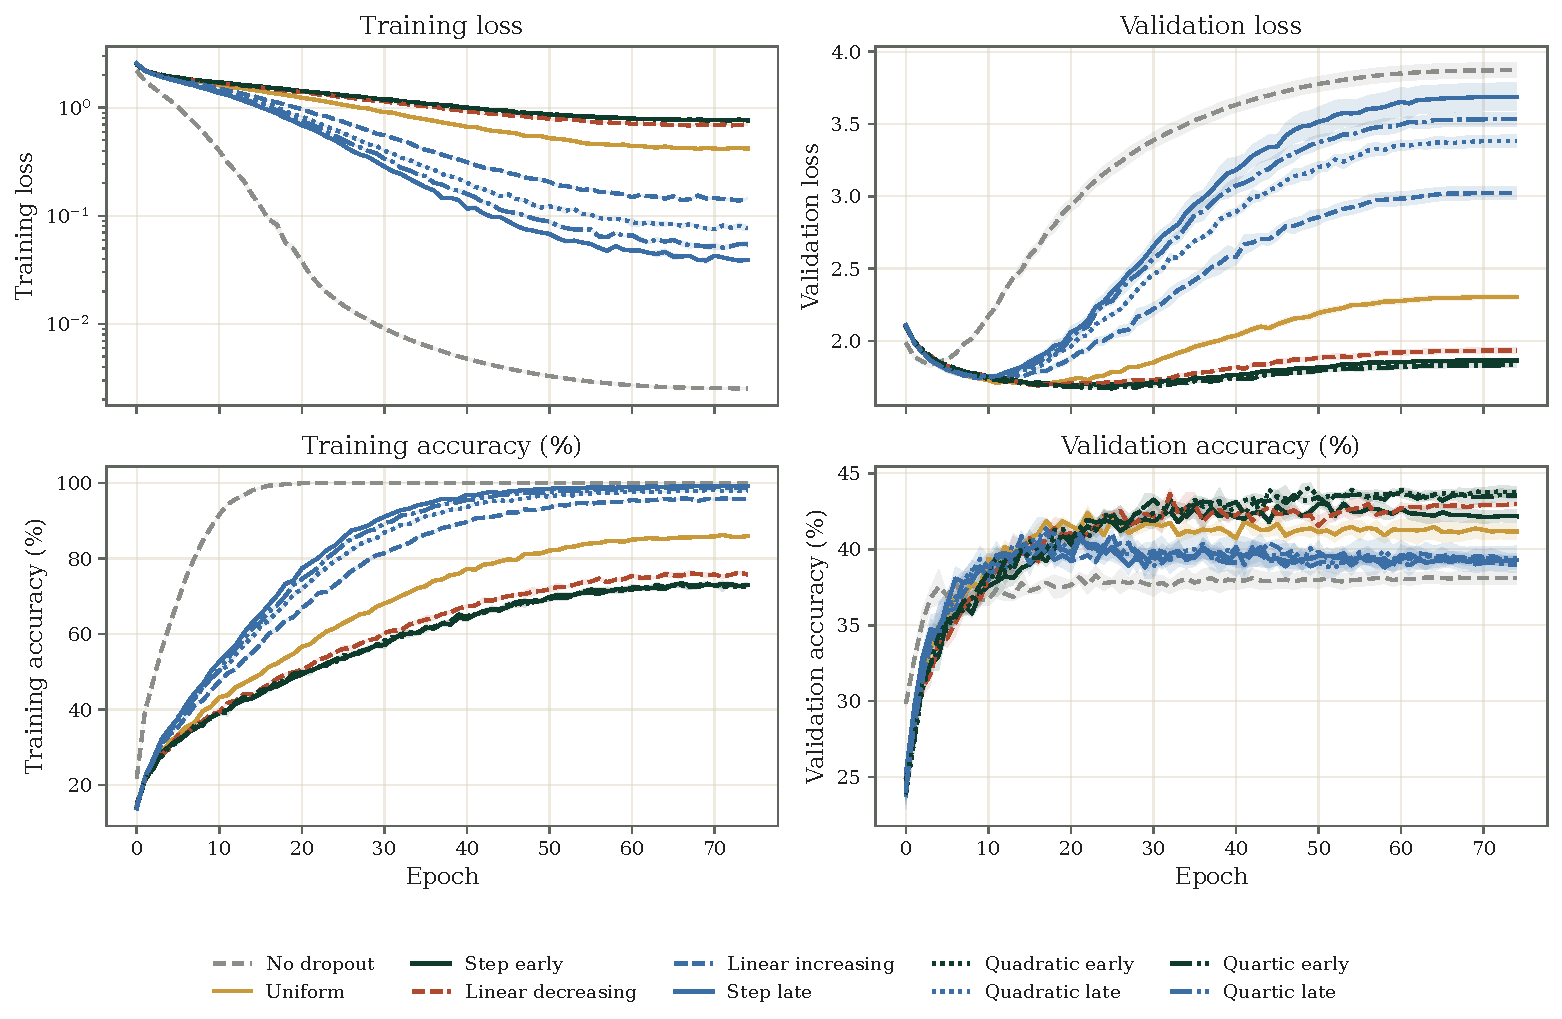
\includegraphics[width=0.94\textwidth]{figures/experiments/benchmarks/profile-geometry-pilot.pdf}
\caption{Profile geometry at fixed mean dropout. Training and validation curves use the original paper style and show mean $\pm$ SEM over three seeds.}
\label{fig:profile-geometry-pilot}\end{figure}
\begin{center}\small\begin{tabular}{@{}lrr@{}}\toprule
Profile & Final validation CE & Final validation accuracy (\%) \\
\midrule
No dropout & \(3.872\pm0.053\) & \(38.10\pm0.40\) \\
Uniform & \(2.303\pm0.019\) & \(41.17\pm0.55\) \\
Step early & \(1.864\pm0.009\) & \(42.17\pm0.43\) \\
Linear decreasing & \(1.933\pm0.019\) & \(42.97\pm0.15\) \\
Linear increasing & \(3.025\pm0.045\) & \(39.30\pm0.40\) \\
Step late & \(3.688\pm0.097\) & \(39.27\pm0.30\) \\
Quadratic early & \(1.852\pm0.001\) & \(43.73\pm0.38\) \\
Quadratic late & \(3.382\pm0.042\) & \(39.43\pm0.80\) \\
Quartic early & \(1.831\pm0.016\) & \(43.53\pm0.41\) \\
Quartic late & \(3.534\pm0.048\) & \(39.00\pm0.50\) \\
\bottomrule\end{tabular}\end{center}
The saved records do not contain a complete width-transfer comparison. The geometry pilot alone does not establish successful $\mu$P transfer.


\end{document}

% This document was modified from the file originally made available by
% Pat Langley and Andrea Danyluk for ICML-2K. This version was created
% by Iain Murray in 2018, and modified by Alexandre Bouchard in
% 2019 and 2021 and by Csaba Szepesvari, Gang Niu and Sivan Sabato in 2022.
% Modified again in 2023 and 2024 by Sivan Sabato and Jonathan Scarlett.
% Previous contributors include Dan Roy, Lise Getoor and Tobias
% Scheffer, which was slightly modified from the 2010 version by
% Thorsten Joachims & Johannes Fuernkranz, slightly modified from the
% 2009 version by Kiri Wagstaff and Sam Roweis's 2008 version, which is
% slightly modified from Prasad Tadepalli's 2007 version which is a
% lightly changed version of the previous year's version by Andrew
% Moore, which was in turn edited from those of Kristian Kersting and
% Codrina Lauth. Alex Smola contributed to the algorithmic style files.
